\documentclass{article}
\setlength{\parskip}{0.25em}

% === Adaptations for publisher submission (highlighted) ===
\usepackage[utf8]{inputenc} % new: ensure standard encoding
\usepackage{geometry} % new: simple page geometry for submission
\geometry{margin=1in} % new: reasonable default margins

% graphics and math (kept)
\usepackage[pdftex]{graphicx}
\graphicspath{{paper/}{paper/figures/}{./}{figures/}}
\DeclareGraphicsExtensions{.pdf,.jpeg,.png}

\usepackage[cmex10]{amsmath}
\usepackage{amssymb} % needed for \mathbb and related symbols
\usepackage{array}
\usepackage{url}

% === Removed nonstandard / IEEE specific packages (they were in original)
% The following were removed to follow the publisher requirement to avoid
% nonstandard packages: mdwmath, mdwtab, eqparbox and others.
% removed: \usepackage{mdwmath}
% removed: \usepackage{mdwtab}
% removed: \usepackage{eqparbox}

% hyphenation line preserved (original)
\hyphenation{op-tical net-works semi-conduc-tor}

% ========== TITLE & AUTHORS ====================================================
\begin{document}

\title{Predictive Multi-Zone Reinforcement Learning Control for Battery Thermal Management}

\author{Mukesh Singh, Keshav Juneja}

\maketitle

% note: replaced IEEE title machinery with standard article title block above.
% All manuscript sentences below are preserved exactly as in your original file.

% === ABSTRACT ====================================================================
\begin{abstract}
Electric vehicle batteries generate considerable heat during operation. Unmanaged heat disturbs electrochemical stability and weakens performance. Traditional controllers react late because they rely only on present sensor readings. They cannot predict temperature evolution or anticipate load induced changes. Their delayed action creates harmful spatial gradients in multi zone packs.

These packs heat unevenly due to non uniform geometry and complex coolant pathways. Spatial gradients form quickly and accelerate long term degradation when not addressed early. Predictive behaviour is therefore essential for safe and efficient operation.

We present Spatial Graph Recurrent Proximal Policy Optimisation, (SGR PPO). It is a predictive reinforcement learning framework for proactive multi zone cooling. The method formulates control as optimisation over future temperature trajectories. It does not rely on instantaneous thermal states. SGR PPO builds a unified state combining spatial graph structure, temporal memory, and global context. This state encodes predicted temperature evolution across all zones.

These predictions directly guide policy optimisation under Proximal Policy Optimisation. The controller therefore acts on anticipated outcomes rather than delayed thresholds.

These predictions directly guide policy optimisation under Proximal Policy Optimisation. Optimisation therefore drives learning by reinforcing actions that improve future thermal outcomes. The controller learns through Proximal Policy Optimisation under demanding conditions. It adjusts coolant flow and valve positions using predicted evolution rather than delayed thresholds.

The architecture contains spatial perception, temporal encoding, and a contextual branch forming a three stage module. A predictive encoder models heat propagation under real conditions. An actor critic controller converts predictions into coordinated thermal actions.

The framework lowers peak temperature, improves spatial uniformity, and reduces auxiliary energy use. Its graph based design scales to large packs with complex internal layouts. The central novelty lies in uniting predictive modelling with multi zone reinforcement learning. This union yields a proactive controller that shapes thermal behaviour before unsafe states arise..
\end{abstract}

% === KEYWORDS ====================================================================
\noindent\textbf{Keywords:} battery cooling, battery thermal management, electric vehicles, multi zone control, predictive control, reinforcement learning, thermal prediction
\clearpage
\twocolumn

% ====================================================================
% ====================================================================
% ====================================================================

% === I. INTRODUCTION =============================================================
\section{Introduction}

The rising concern over fossil fuel emissions has increased interest in electric vehicles.
These vehicles draw power from cleaner sources and support long term carbon neutrality goals.
A detailed comparison of vehicle emissions appears in the work of Wang et al. who analysed realistic driving use \cite{LCA_EV2023}.
Government incentives further support electric vehicle adoption by reducing effective purchase cost for new buyers.
The expected decline in battery prices has been examined through learning curve analysis.
This analysis appears in the work of Link et al. which relates pack cost to manufacturing scale \cite{Link2024}.
Higher adoption increases the demand for lithium ion batteries across multiple vehicle classes.
These batteries generate heat during charge and discharge cycles because internal processes release thermal energy.
High load currents increase resistive heating within electrodes and current collectors.
Extreme ambient temperatures further push cells away from their recommended thermal range.
The effect of thermal gradients has been examined through combined experiments and modelling.
This effect was quantified in the work of Zang et al. who observed reduced performance under gradients \cite{ThermalGradients2023}.
Prolonged exposure to unsafe temperatures increases the risk of thermal runaway events.
Battery Thermal Management Systems therefore play a central role in safety and reliability.
They also preserve consistent performance over the operational lifetime of the pack.

Researchers typically classify BTMSs rule based, optimisation based, and learning based categories.
Rule based controllers rely on fixed logic and predefined temperature thresholds.
They behave adequately under steady loads and low spatial variation.
Their behaviour degrades under rapid load changes or uneven heating across the pack.
This limitation was demonstrated using multi zone experiments.
These experiments appear in the work of Xu et al. who observed strong temperature differences across zones \cite{Xu2019Thermoelectric}.
Optimisation based controllers compute cooling actions using mathematical cost functions and physical constraints.
They perform well when the model accurately represents real pack behaviour.
Model mismatch reduces prediction accuracy and degrades transient response.
High computation cost also limits deployment in real time automotive systems.
Learning based controllers adjust behaviour from observed data and past operation.
They reduce dependence on explicit plant models and respond better to unmodelled dynamics.
The benefits of learning based adaptation were demonstrated in the work of Ortiz Arevalo et al. who evaluated dynamic driving conditions \cite{OrtizArevalo2024}.
Their controller maintained safer temperatures under aggressive load changes.

\subsection{Literature Review}

Thermal modelling for battery packs uses analytical models, data driven models, and hybrid methods.
Analytical models approximate heat transfer with simplified geometry and reduced physics.
These models run quickly but omit important spatial detail inside the pack.
Data driven models learn patterns from operational measurements across many cycles.
Hybrid models combine physics components with learned structures for improved accuracy.
Popular tools include PyBaMM and LIONSIMBA for thermal and electrochemical studies.
These tools accelerate experiments but they introduce abstractions that can obscure mechanisms.
Recent work compares convolutional, graph, and physics informed neural architectures.
See Liu et al. \cite{Liu2024} for such comparisons.
Physics informed networks embed governing equations within the loss during training.
This improves physical consistency and reduces pure data requirements.
They still need diverse datasets for robust performance.
Interpreting internal mechanisms remains challenging for engineers.

AI controllers extend classical control with learned policies and feedback augmentation.
A neural network combined with PID reduced coolant energy use by 17.6 percent \cite{Batteries2023}.
Deterministic policy gradients improved regulation in prior studies \cite{ESWA2025}.
Adaptive model predictive control with actor critic methods showed fewer thermal violations \cite{Wu2025}.
Attention based reinforcement learning improved energy efficiency in multi scenario tests \cite{Cao2025}.
Reinforcement learning also supports automatic PID tuning via recurrent and convolutional modules \cite{Rudolf2024}.
Simple learning controllers outperform fixed logic in single zone systems \cite{11017253}.
The literature shows clear progress, yet limits remain in spatial precision and forecasting.

\subsection{Research Gap}

Reactive controllers act only after temperatures exceed safety thresholds.
This delayed action allows hotspots to grow and form damaging spatial gradients.
These gradients intensify thermal stress and accelerate degradation.
Predictive control acts earlier to prevent such damage.
Rudolf et al. tuned PID using learned thermal trends and reported benefits \cite{Rudolf2024}.
However, PID cannot manage non uniform heating in multi zone packs.
Multi zone packs need coordinated decisions that account for spatial coupling.
Recent reinforcement learning controllers improve adaptability but retain shortcomings.
Memory based RL adds temporal reasoning yet does not address spatial precision \cite{Huang2022}.
Hierarchical temporal optimisation improved violation handling, but lacked hotspot forecasting \cite{Wu2025}.
Attention models often use averaged pack values, hiding local variations \cite{Cao2025}.
Hybrid RL controllers showed mixed reactive behaviour without genuine prediction \cite{Rudolf2024}.
No published work fully integrates predictive modelling with multi zone RL.
No real time control pipeline offers spatial precision at practical scale.
These gaps motivate a predictive multi zone controller for battery packs.

\subsection{Motivation}

Existing controllers struggle coordinating cooling across many thermally coupled zones.
This arises because spatial interaction and temporal evolution are handled separately.
A unified representation is required to reason about heat propagation.
Graph based modelling naturally captures spatial coupling between neighbouring cells.
Recurrent temporal encoding represents delayed thermal responses under load changes.
Global context influences cooling effectiveness through ambient and vehicle conditions.
Reinforcement learning optimises control under coupled dynamics and practical constraints.
Proximal Policy Optimisation offers stable learning for continuous actions in real time.
These considerations motivate our predictive reinforcement learning framework.
Integration enables coordinated and anticipatory thermal control across zones.

\subsection{Contributions}

\begin{enumerate}
\item We introduce a predictive thermal representation combining spatial graphs and temporal recurrence.
      It forms a compact latent state for multi zone temperature forecasting.
\item We develop a reinforcement learning controller trained with Proximal Policy Optimisation.
      This enables stable optimisation of continuous cooling actions under long horizon objectives.
\item We integrate prediction and control into one real time framework.
      The framework coordinates valves and flow to improve uniformity and reduce energy use.
\end{enumerate}


\begin{figure*}[t]
    \centering
    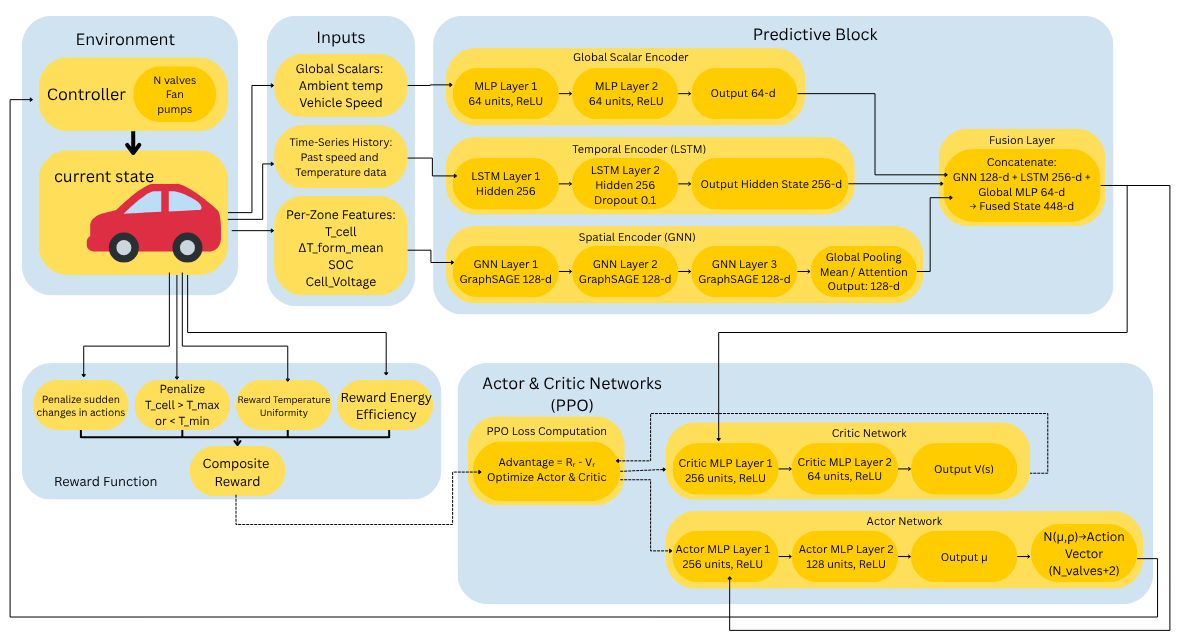
\includegraphics[width=\textwidth]{iter3.png}
    \caption{Architecture of the proposed reinforcement learning based battery thermal management system, integrating predictive encoding, multi zone perception, and actor–critic control for proactive, energy efficient temperature regulation.}
    \label{fig:architecture}
\end{figure*}


% === VI. Proposed Framework =============================================================
\section{Proposed Framework}

This section presents the control framework developed in this study.
Figure \ref{fig:architecture} illustrates the complete control loop executed at each time step.
The loop begins with measurements obtained from the battery pack and operating environment.
These measurements are organised into structured inputs for spatial, temporal, and global processing.
A predictive block processes the inputs to estimate future thermal behaviour across zones.
This prediction captures heat propagation and delayed thermal response under dynamic conditions.
An actor critic controller then computes continuous control actions based on the predicted state.
These actions regulate valve positions, coolant flow rate, and fan speed within the system.
The applied actions influence temperature evolution during the next interval.
Updated measurements are returned to the controller, closing the loop.
This repeated interaction enables coordinated and anticipatory cooling in multi zone battery packs.
The framework is organised into four components.
These components are the Environment, the Inputs, the Predictive Block, and the Actor Critic Module.
Each component is described in detail in the following subsections.

\subsection{Environment}

In Figure \ref{fig:architecture}, the environment forms the outer structure of the loop.
This environment represents an electric vehicle pack with many coolant channels.
Each channel contains a valve that meters coolant distribution across zones.
A pump and a fan maintain circulation and heat rejection.
Temperatures, loads, and ambient conditions reach the controller continuously.
The simulator produces spatial heat generation models that capture uneven heating.
Coolant transport and actuator latency also appear within this simulation.
Latency affects timing during real time control and must be learned.
Training occurs entirely inside this simulated environment before evaluation.

\subsection{Inputs}

The three input groups shown in Figure \ref{fig:architecture} provide multi scale context for control.
Global scalars supply ambient temperature and vehicle speed.
These values describe broad operating conditions surrounding the pack.
Short histories track recent temperature and speed evolution.
Through these histories, the controller perceives rising heat or falling load.
Per zone features then reveal local thermal differences between cells.
These features include cell temperature, formation mean, SOC, and voltage.
This three part design links global behaviour with local thermal variation.
Uneven heating across zones becomes visible through this structure.

\subsection{Predictive Block}

Within Figure \ref{fig:architecture}, the predictive block merges all inputs into one latent state.
Scalar features enter two MLP layers that each use width 64.
This width provides balanced expressiveness under tight computational limits.
Temporal information moves through a two layer LSTM with hidden size 256 and dropout 0.1.
This configuration captures delayed heating and cooling patterns within short histories.
Spatial structure enters three GraphSAGE layers with 128 dimensional embeddings.
These embeddings model heat propagation between neighbouring cells.
A global pooling layer compresses node outputs into a 128 dimensional spatial summary.
The scalar, temporal, and spatial embeddings then fuse into one 448 dimensional latent state.
This latent state serves as the predictive foundation for control.

\subsection{Actor and Critic Networks with PPO}

The fused state in Figure \ref{fig:architecture} flows into the actor and critic paths.
Two fully connected layers with sizes 256 and 64 estimate value within the critic.
The actor mirrors this structure and outputs a mean action vector.
This vector defines a Gaussian distribution over all actuator commands.
Action dimension equals the number of valves plus 2 actuator channels.
Training follows clipped Proximal Policy Optimization for stable improvement.
The advantage term uses the difference between observed return and predicted value.

\subsection{Reward Function}

The reward path in Figure \ref{fig:architecture} gathers objectives required for safe cooling.
Safety penalties activate when temperatures exit permitted cell ranges.
Uniformity penalties reduce temperature variance between zones.
Energy penalties measure auxiliary power from pumps and fans.
Smoothness penalties discourage abrupt movements in actuators.
These terms promote early intervention and efficient thermal regulation.

\subsection{Overall Operation}

The closed loop behaviour in Figure \ref{fig:architecture} unites all previous components.
The predictive block forecasts temperature evolution at each step.
The actor proposes commands for valves, pumps, and fans.
The critic evaluates these actions during training and guides improvement.
The simulated environment then applies commands and returns new measurements.
This cycle repeats at every control interval with updated data.
Proactive cooling emerges from this arrangement across dynamic driving conditions.
Temperature uniformity and safety remain preserved across zones.
The design scales naturally to larger packs without major structural change.

\section{BTMS Control Model}

This section formalises predictive thermal regulation.
The formulation matches the SGR PPO architecture.
Control is expressed over future temperature evolution.
The structure unifies physics and policy optimisation.
Explanatory text clarifies each modelling choice and implication.

\subsection{Control Architecture Overview}

The control loop links thermal dynamics and the agent.
The thermal state is denoted by \(x_t\).

System evolution follows

\begin{equation}
x_{t+1} = f(x_t, a_t, u_t).
\end{equation}

State \(x_t\) contains thermal and electrical variables.
Action \(a_t\) defines continuous cooling commands.
Input \(u_t\) captures ambient and operating conditions.
Function \(f(\cdot)\) encodes electrothermal evolution.
The model combines physics and data driven approximations.
Learning adjusts parameters to fit observed transitions.

The controller receives measurable quantities only.
Internal states remain partially observed.

Observations follow

\begin{equation}
o_t = g(x_t, u_t),
\end{equation}

Function \(g(\cdot)\) selects sensed variables.
Observation \(o_t\) includes temperature measurements and global context.
Sensor noise and sampling delay are modelled implicitly.

\subsection{Observation Construction}

Thermal behaviour exhibits spatial structure.
Cells exchange heat through conduction paths.
A graph representation captures this topology and neighbourhood relations.
Nodes represent cells, with local measurements and metadata.
Edges encode conductive coupling and physical separation.

Node features for cell \(j\) are

\begin{equation}
x^{\mathrm{node}}_j =
\bigl[T_{b,j},\ T_{b,j}-\bar T_b,\ \mathrm{SOC}_j,\ I_{\mathrm{pack}},\ V_j,\ s_j\bigr].
\end{equation}

These features mix absolute and relative temperature signals.
Pack current is treated as spatially uniform.

Edge features between cells \(i\) and \(j\) are

\begin{equation}
x^{\mathrm{edge}}_{i\to j} =
[d_{ij},\ k^{\mathrm{cond}}_{ij}].
\end{equation}

Distance and conductance quantify pair wise coupling.

Temporal context captures thermal momentum.
Temperature evolves under sustained load.
Short term history therefore improves predictive accuracy.

Temporal history is

\begin{equation}
x^{\mathrm{hist}} =
\bigl[\bar T_b^{\,t-K+1:t},\
T_{b,\max}^{\,t-K+1:t},\
T_{b,\min}^{\,t-K+1:t},\
I_{\mathrm{pack}}^{\,t-K+1:t}\bigr].
\end{equation}

Window length K is chosen by cross validation.
History feeds the temporal encoder for learned dynamics.

Global context affects cooling effectiveness.

Global scalars are

\begin{equation}
x^{\mathrm{glob}} =
[T_{\mathrm{amb}},\ v_{\mathrm{veh}},\ \mathbb{1}_{\mathrm{HVAC}}].
\end{equation}

Vehicle speed modulates convective rejection rates.
HVAC activity indicates compressor assisted cooling.

\subsection{Predictive Encoders}

Spatial perception uses GraphSAGE layers.

\begin{align}
H^{(1)} &= \sigma(\mathrm{SAGE}(X^{\mathrm{node}}, X^{\mathrm{edge}}; \theta_1)),\\
H^{(2)} &= \sigma(\mathrm{SAGE}(H^{(1)}; \theta_2)),\\
H^{(3)} &= \sigma(\mathrm{SAGE}(H^{(2)}; \theta_3)).
\end{align}

Stacking multiplies receptive fields across the graph.
Global pooling produces

\begin{equation}
z_g = \mathrm{Pool}(H^{(3)}).
\end{equation}

This vector summarises pack level structure.

Temporal encoding uses recurrent memory.

\begin{equation}
z_t \in \mathbb{R}^{256}.
\end{equation}

This vector stores learned thermal evolution.
Global scalars pass through a multilayer encoder.

\begin{equation}
z_s = \phi_2(\phi_1(x^{\mathrm{glob}})).
\end{equation}

The unified predictive state is

\begin{equation}
z = \mathrm{concat}(z_g, z_t, z_s).
\end{equation}

This state encodes predicted multi zone behaviour.
This state conditions both actor and critic networks.

\subsection{Actor and Critic Networks}

Cooling commands operate over continuous ranges.
A Gaussian policy enables smooth exploration.

The actor produces

\begin{align}
\mu &= \psi_{\mu}(z),\\
\log \sigma &= \psi_{\sigma}(z).
\end{align}

Parameters \(\mu\) and \(\log \sigma\) drive sampling.
Sampling yields actions, which are then projected.
The critic outputs a state value estimate.

\begin{equation}
V_{\phi}(o_t) = \chi(z).
\end{equation}

Both networks are trained jointly using PPO.
Training uses batched on policy rollouts and advantage estimation.
Regularisation and early stopping control overfitting.

\subsection{Action Constraints}

Neural outputs are unconstrained by design.
Physical actuators obey strict limits and safety bounds.
Squashing functions map outputs into admissible ranges.

\begin{align}
\alpha_i &= \sigma(\tilde \alpha_i),\\
q_{\mathrm{pump}} &=
q_{\min} + (q_{\max}-q_{\min})\,\sigma(\tilde q),\\
\omega_{\mathrm{fan}} &=
\omega_{\max}\,\sigma(\tilde \omega).
\end{align}

Effective conductance modulation replaces explicit flow allocation.
This simplification reduces model complexity and runtime cost.
Hardware safety checks clamp commands before execution.

\subsection{Reward Function}

The objective balances safety, uniformity, and energy efficiency.

Safety term

\begin{equation}
r_{\mathrm{safe}} =
-\lambda_1 \sum_j \max(0,T_{b,j}-T_{\max})
-\lambda_2 \sum_j \max(0,T_{\min}-T_{b,j}).
\end{equation}

This term penalises cells exceeding safety bounds.
Uniformity term

\begin{equation}
r_{\mathrm{temp}} =
-\lambda_3\,\mathrm{Var}\{T_{b,j}\}.
\end{equation}

Variance penalisation encourages even temperature distribution.
Energy term

\begin{equation}
r_{\mathrm{energy}} =
-\lambda_4\,P_{\mathrm{aux}}.
\end{equation}

Auxiliary power captures cooling cost in real units.
Smoothness term

\begin{equation}
r_{\mathrm{smooth}} =
-\lambda_5\,\lVert a_t - a_{t-1}\rVert_2^2.
\end{equation}

Action smoothness reduces actuator wear and oscillation.
Total reward is

\begin{equation}
r_t =
w_{\mathrm{safe}} r_{\mathrm{safe}}
+ w_{\mathrm{temp}} r_{\mathrm{temp}}
+ w_{\mathrm{energy}} r_{\mathrm{energy}}
+ w_{\mathrm{smooth}} r_{\mathrm{smooth}}.
\end{equation}

Weights tune priorities during training and deployment.
Reward shaping uses curriculum scheduling when necessary.

\subsection{Thermal Dynamics}

Cell temperature follows energy conservation.

\begin{equation}
C_{b,j}\frac{dT_{b,j}}{dt}
=
\dot Q_{\mathrm{gen},j}
-
\dot Q_{\mathrm{cool},j}
+
\sum_{k\in\mathcal{N}(j)}
k_{jk}(T_{b,k}-T_{b,j}).
\end{equation}

Conductive exchange uses neighbourhood topology and conductance weights.
Thermal capacitance aggregates per cell or zone.

\begin{equation}
C_{b,j} =
n_{\mathrm{cells},j} C_{\mathrm{cell}}.
\end{equation}

Heat capacity scales with the cell count per zone.

\begin{equation}
\dot Q_{\mathrm{gen},j} =
I_{\mathrm{pack}}^2 R_j.
\end{equation}

Resistive heating uses pack current and local resistance.
Entropic and regenerative heating are omitted for baseline.

\begin{equation}
\dot Q_{\mathrm{cool},j} =
U_j A_j (T_{b,j} - T_{\mathrm{cool}}).
\end{equation}

Lumped UA form approximates convective heat transfer.

\begin{equation}
U_j =
\beta_{0,j}
+
\beta_{1,j}\dot m_{\mathrm{tot}}^{\eta_j}
+
\beta_{2,j}\omega_{\mathrm{fan}}^{\zeta_j}.
\end{equation}

Conductance depends on total flow and fan speed.
This modelling choice simplifies per branch dynamics into control inputs.

\subsection{Learning Objective}

Advantage estimation uses generalized advantage estimation.

\begin{align}
\hat A_t &=
\sum_{l=0}^{L-1}
(\gamma\lambda_{\mathrm{GAE}})^l
\delta_{t+l},\\
\delta_t &=
r_t + \gamma V_{\phi}(o_{t+1})
- V_{\phi}(o_t).
\end{align}

GAE trades bias and variance in advantage estimates.
Policy ratio is

\begin{equation}
\rho_t(\theta) =
\frac{\pi_{\theta}(a_t \mid o_t)}
{\pi_{\theta_{\mathrm{old}}}(a_t \mid o_t)}.
\end{equation}

Clipped objective is

\begin{equation}
\mathcal{L}_{\mathrm{policy}} =
\mathbb{E}
\left[
\min
\left(
\rho_t \hat A_t,
\mathrm{clip}(\rho_t,1-\epsilon,1+\epsilon)\hat A_t
\right)
\right].
\end{equation}

Clipping stabilises updates and prevents large policy shifts.
Value and entropy terms regularise learning and exploration.

\begin{align}
\mathcal{L}_V &= \mathbb{E}[(V_{\phi}(o_t) - \hat V_t)^2],\\
\mathcal{L}_{\mathrm{ent}} &= \mathbb{E}[\mathcal{H}(\pi_{\theta}(\cdot \mid o_t))].
\end{align}

The total objective balances optimisation and robustness.
Training schedules and hyper parameter sweeps find practical settings.

\bigskip

\noindent\textbf{Implementation notes.}
\begin{itemize}
  \item Entropic and regenerative heating are omitted in the baseline.
  \item Cooling uses lumped conductance, tied to global pump and fan commands.
  \item Lateral conduction captures spatial diffusion across neighbouring cells.
  \item Per branch mass flow allocation is replaced by conductance modulation.
\end{itemize}
\section{Results}
\subsection{Drive cycles and preprocessing}

The dataset uses regulatory schedules published by United States environmental agencies.\cite{EPA_Dynamometer}
These schedules cover dense traffic, cruising, acceleration, and cabin cooling operation conditions.\cite{DieselNet_Cycles}
We selected every schedule file in the drive cycles folder except the merged file.
This choice avoids repeated patterns that could bias comparison between control strategies.
The retained schedules include FTP, UDDS, HWFET, US06, SC03, and LA92 traces.
Each schedule contributes distinct speed transitions and dwell periods across the evaluation horizon.
City focused traces emphasize frequent stopping, restart behavior, and short transient bursts.
Highway traces emphasize sustained speed, smoother profiles, and long thermal loading periods.
Aggressive traces increase acceleration peaks and expose stronger heat generation under high current.
Air conditioning traces introduce added auxiliary demand during warmer ambient operating windows.
Together these schedules create broad operating coverage for robust thermal controller assessment. Coverage across operating modes improves confidence when comparing controllers under shared constraints. It also reduces selection bias from narrow schedule composition. This diversity reflects realistic daily driving behavior across many urban and highway contexts. Results therefore generalize better across usage patterns than single cycle evaluation.

Raw schedule files were parsed into synchronized time and speed records before modeling.
Non numeric entries were removed to prevent parser failures during feature construction.
Timestamp inconsistencies were corrected using monotonic ordering and fixed interval resampling.
We applied controlled smoothing to suppress numerical spikes while preserving transient behavior.
Vehicle longitudinal equations converted speed traces into traction power demand profiles.
Electrical current estimates were derived from power demand and pack voltage assumptions.
Estimated currents were clipped within realistic pack limits used during controller training.
Feature windows used fixed history length and fixed prediction horizon across all methods.
Chronological splits separated training, validation, and testing windows without temporal leakage.
All preprocessing steps matched the method section definitions for strict protocol consistency.
This protocol supports reproducible comparison and clear interpretation of downstream results. Consistent preparation makes differences easier to attribute to controller design, not data artifacts. It also improves fairness across training and testing partitions. Stable preprocessing reduces variance in observed thermal trajectories and auxiliary demand estimates. These controls strengthen methodological trust in the reported findings.

\subsection{Comprehensive performance evaluation}

All controllers were evaluated under identical trajectories, weather assumptions, and initial pack states.
We report peak temperature, mean temperature, spread, cooling energy, and overhead indicators.
Each metric captures a different operational concern during battery thermal management deployment.
Peak temperature reflects safety margin under harsh demand and elevated ambient conditions.
Mean temperature reflects sustained thermal burden experienced through most operating intervals.
Spread captures pack uniformity, which affects aging balance and reliability outcomes.
Cooling energy reflects auxiliary consumption driven by pumps, fans, and flow allocation choices.
Overhead normalizes cooling energy against propulsion demand for mission level interpretation.
Figures are discussed in ordered groups to maintain a clear narrative progression.
Each group links quantitative patterns with practical controller selection implications.
This structure reduces repetition while preserving detail needed for technical assessment. Ordered discussion also helps readers map each claim to corresponding visual evidence. The approach keeps narrative flow aligned with figure progression. It prevents repeated explanations of the same metric behavior across adjacent sections. This organization supports faster review and clearer technical traceability.

\subsubsection{Energy and temperature trade off}

\begin{figure}[htbp]
    \centering
    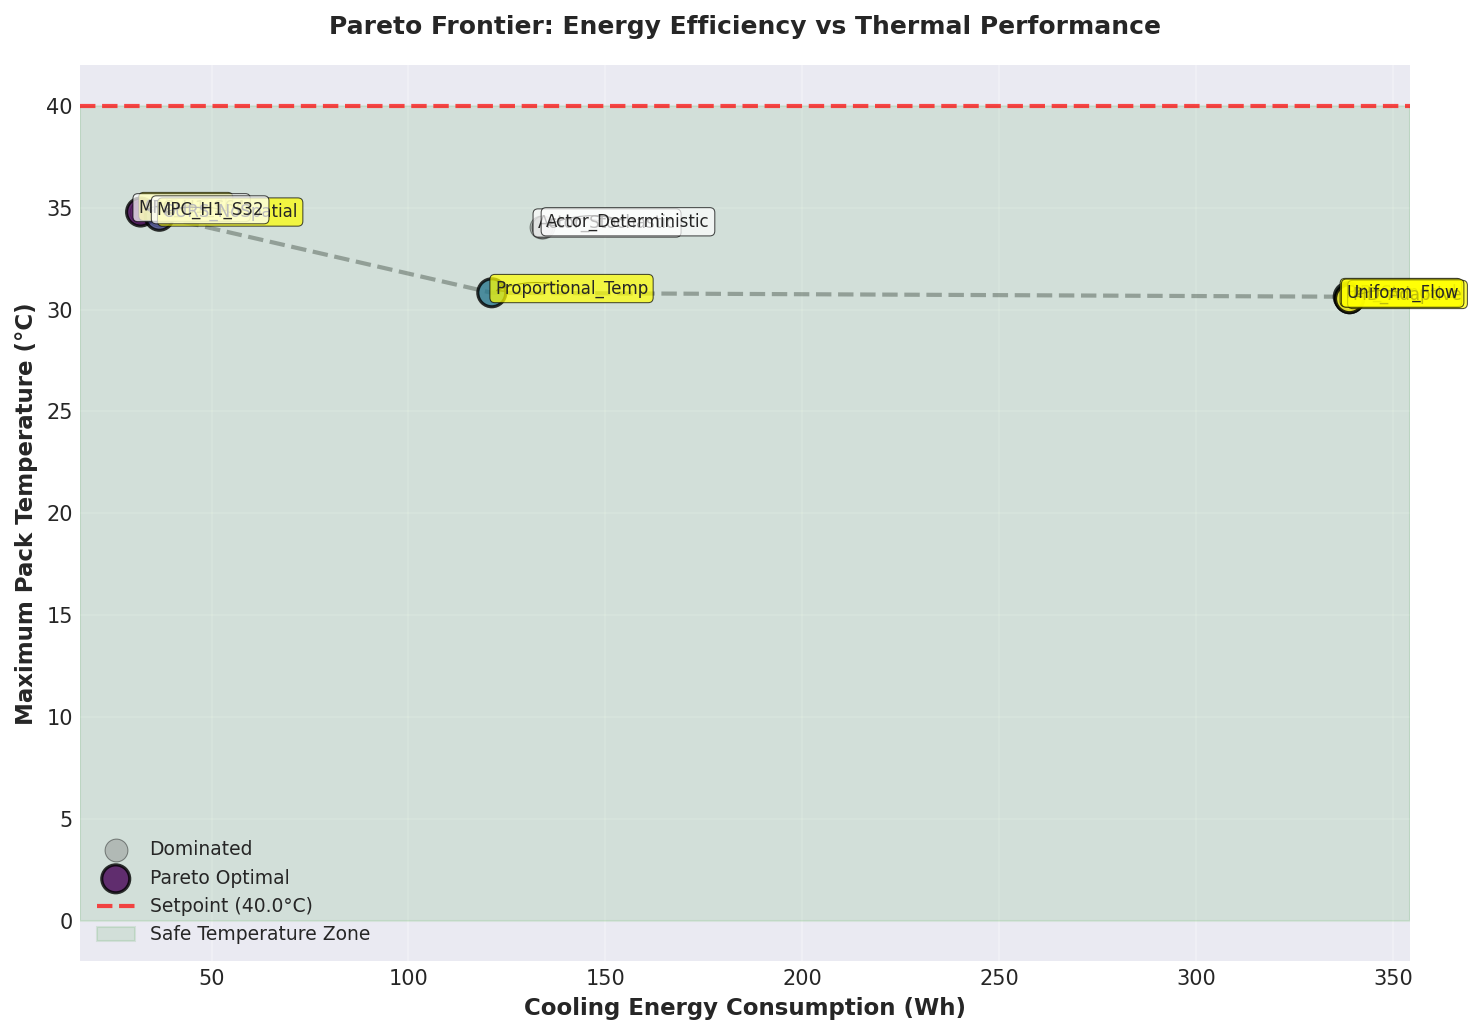
\includegraphics[width=0.8\linewidth]{pareto_frontier.png}
    \caption{Pareto frontier showing energy consumption versus maximum temperature.}
    \label{fig:pareto_frontier}
\end{figure}

Figure \ref{fig:pareto_frontier} maps cooling energy against maximum temperature for all controllers.
Points near the lower left indicate stronger efficiency and safety compromise quality.
OURS Full and MPC variants remain close to this desirable frontier region.
These methods limit auxiliary energy while keeping peak temperature inside acceptable bounds.
Proportional Temp achieves the lowest peak temperature among tested controller families.
Its stronger corrective behavior requires higher auxiliary energy over the full trajectory.
PID variants remain thermally safe but consume substantially larger cooling energy budgets.
This separation confirms a clear efficiency and conservatism trade across control styles.
Range focused deployment should prioritize frontier points with lower auxiliary burden.
Safety focused deployment can accept higher energy for stronger thermal margin.
The frontier therefore guides explicit policy selection under mission specific operating priorities. Teams can set acceptable peak limits first, then choose the lowest energy option. Alternative priorities can invert this choice when safety margin dominates. The plot also reveals when methods provide similar safety with different energy penalties. That insight supports transparent controller justification during design review.

\subsubsection{Temporal response analysis}

\begin{figure}[htbp]
    \centering
    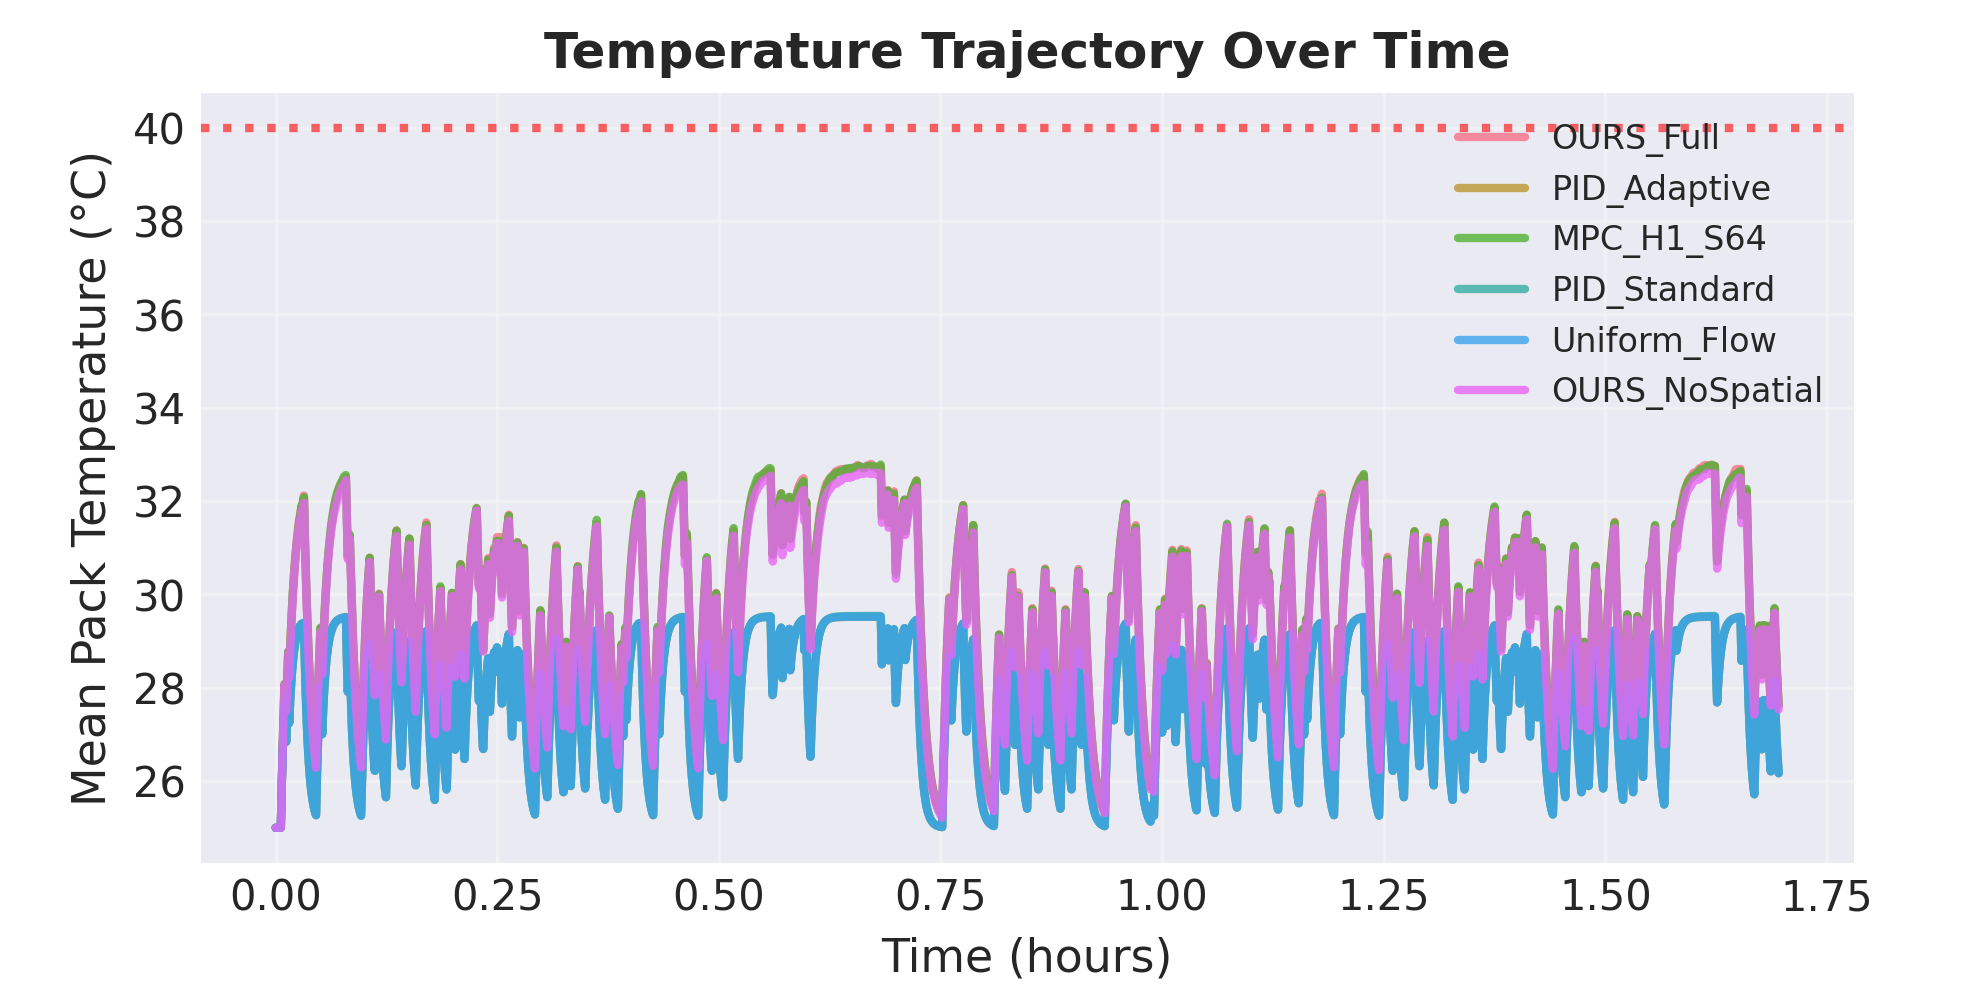
\includegraphics[width=0.8\linewidth]{analysis_temporal_dashboard_r1c1.png}
    \caption{Temporal panel one. Mean pack temperature trajectory over time.}
    \label{fig:temporal_r1c1}
\end{figure}

\begin{figure}[htbp]
    \centering
    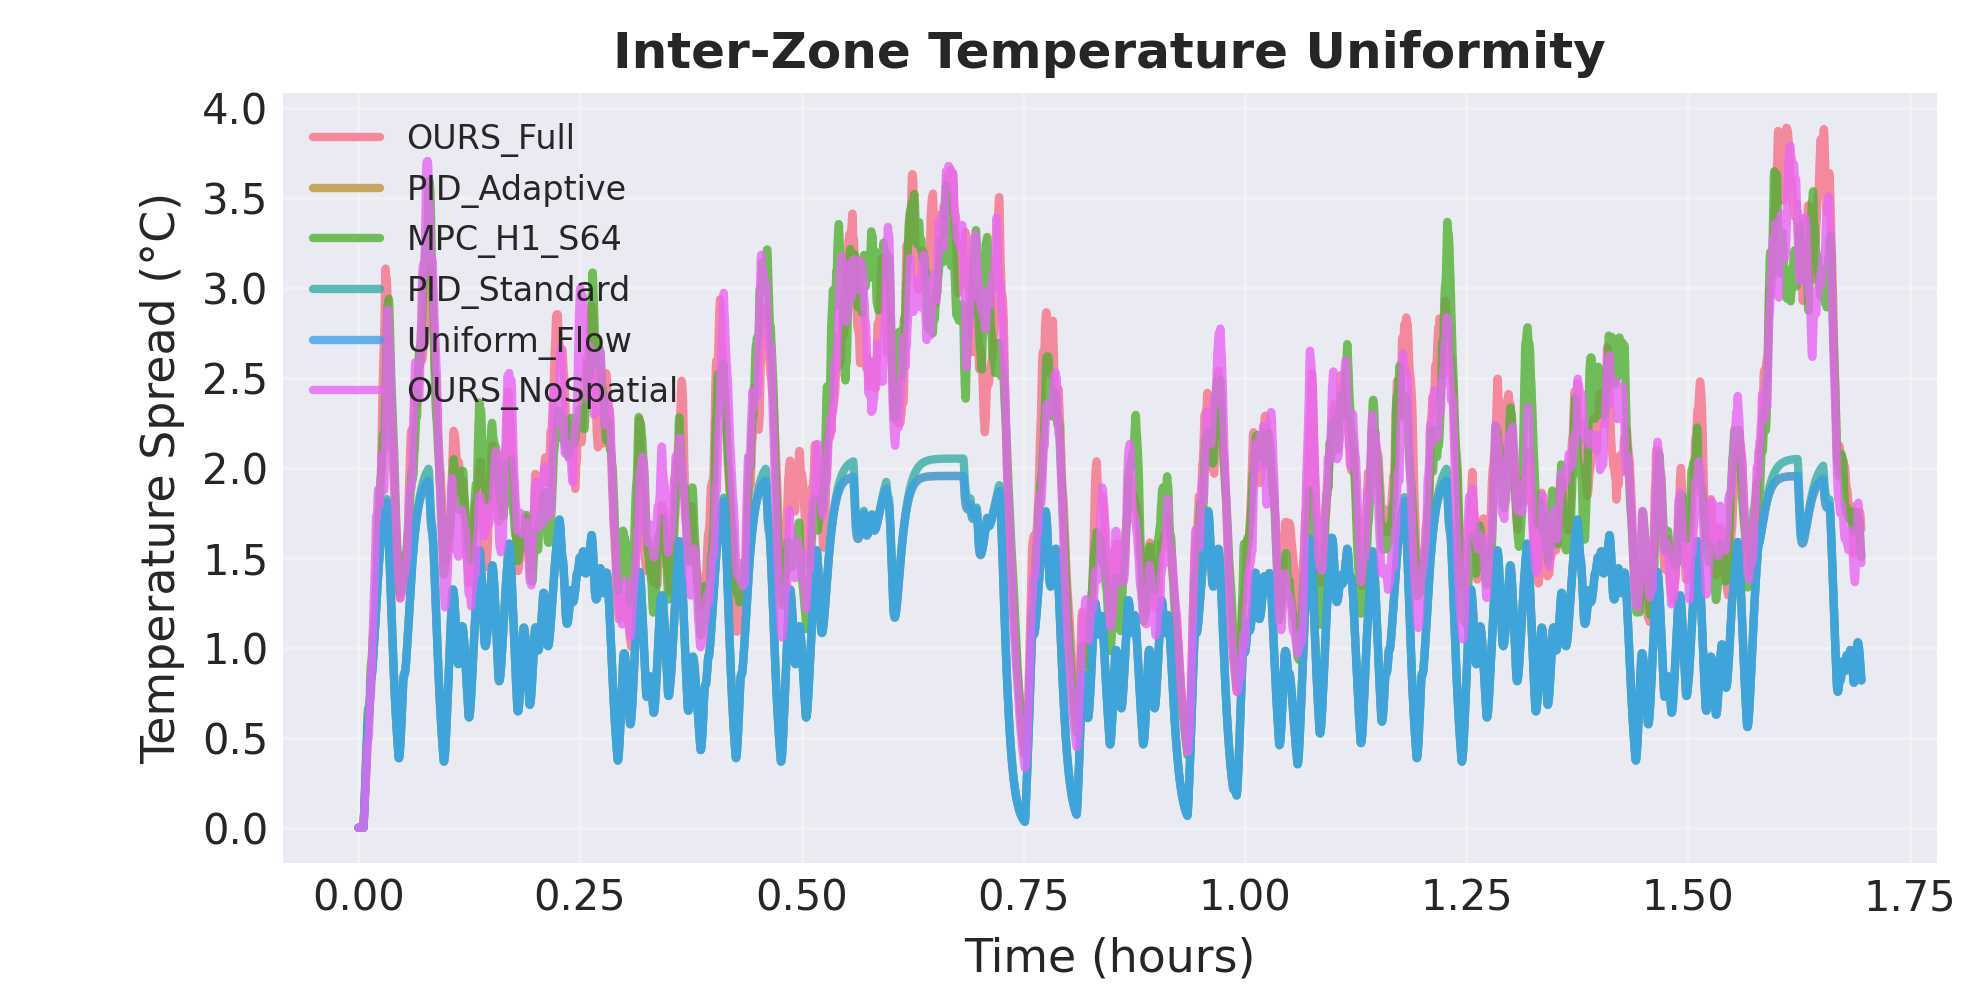
\includegraphics[width=0.8\linewidth]{analysis_temporal_dashboard_r1c2.png}
    \caption{Temporal panel two. Inter zone temperature spread over time.}
    \label{fig:temporal_r1c2}
\end{figure}

\paragraph{Mean temperature and spread}
Figures \ref{fig:temporal_r1c1} and \ref{fig:temporal_r1c2} describe average temperature and spread evolution.
Mean temperature remains stable for all methods across most operating intervals.
Differences appear during rapid demand ramps and recovery periods after heavy loading.
Predictive methods anticipate heating and begin moderation before strong excursions develop.
Proportional control reacts quickly when local temperature rises become immediately visible.
PID strategies apply conservative action and hold cooling longer during transients.
Longer cooling windows reduce excursions but increase auxiliary effort during later intervals.
Spread trajectories show proportional control keeps tighter uniformity for extended periods.
Predictive policies tolerate mild spread when energy savings become operationally valuable.
This behavior indicates explicit balancing between uniformity and efficiency objectives.
These panels establish baseline temporal behavior before deeper energy and stress examination. They also highlight when control divergence begins during the trajectory timeline. Early divergence often predicts later energy and reliability outcomes. Observing both signals together improves diagnosis of policy strengths and weaknesses. This pairing forms a strong foundation for subsequent temporal comparisons.

\begin{figure}[htbp]
    \centering
    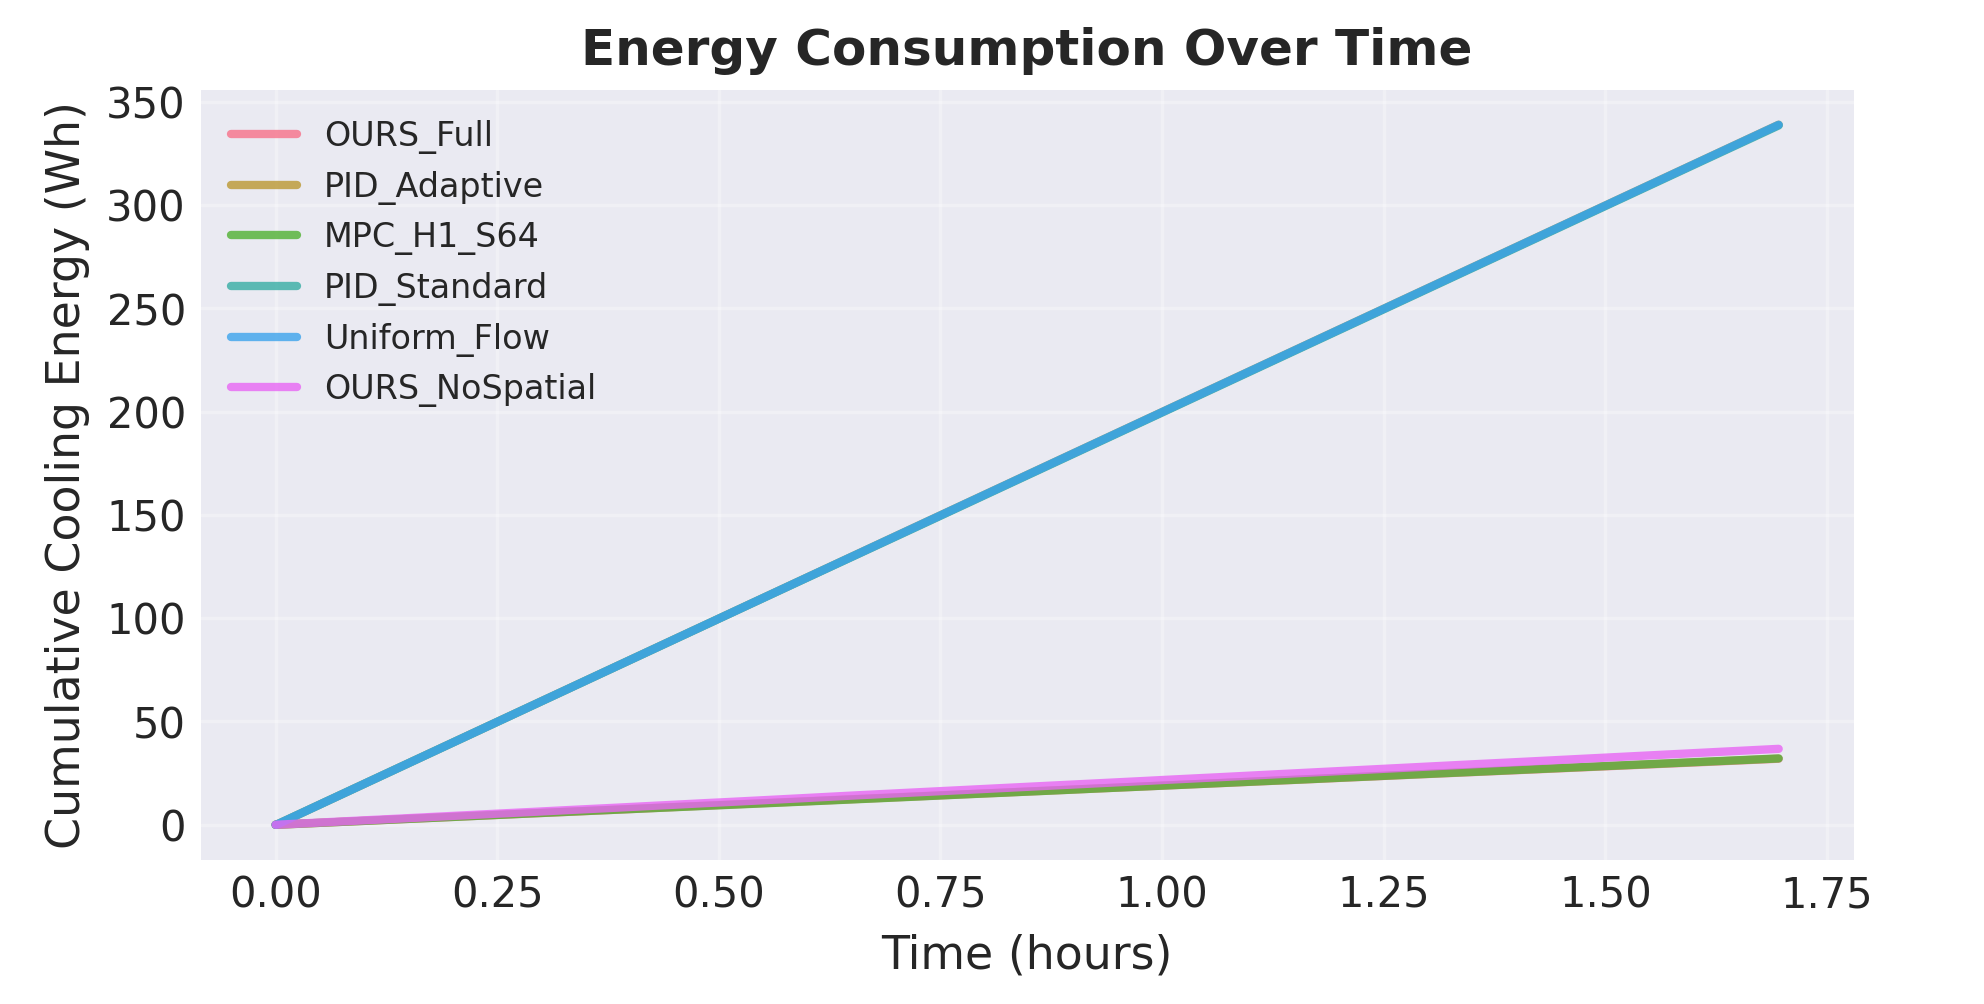
\includegraphics[width=0.8\linewidth]{analysis_temporal_dashboard_r2c1.png}
    \caption{Temporal panel three. Cumulative cooling energy over time.}
    \label{fig:temporal_r2c1}
\end{figure}

\begin{figure}[htbp]
    \centering
    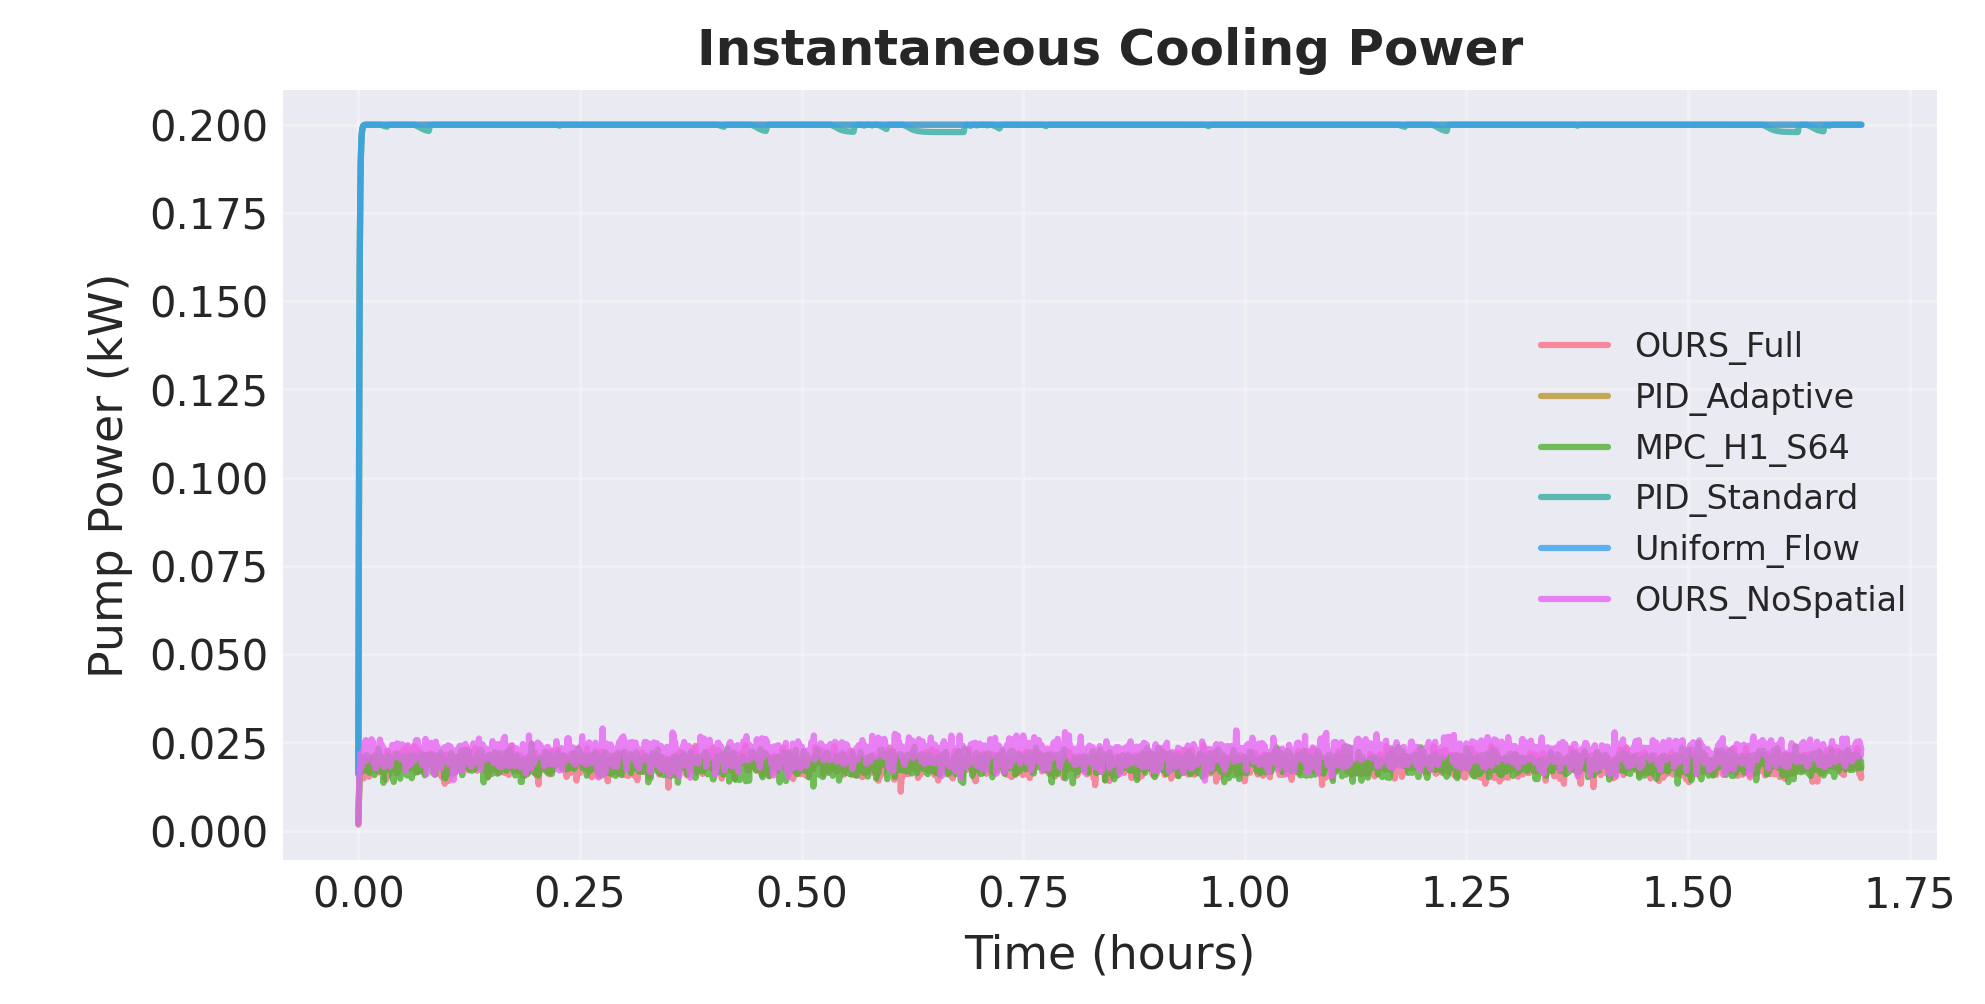
\includegraphics[width=0.8\linewidth]{analysis_temporal_dashboard_r2c2.png}
    \caption{Temporal panel four. Instantaneous cooling power over time.}
    \label{fig:temporal_r2c2}
\end{figure}

\paragraph{Cumulative energy and power demand}
Figures \ref{fig:temporal_r2c1} and \ref{fig:temporal_r2c2} quantify cumulative and instantaneous cooling demand.
Cumulative curves reveal total auxiliary burden accumulated across the drive horizon.
PID curves rise steeply, reflecting persistent and conservative cooling behavior.
Predictive curves rise gradually with fewer large increments during dynamic phases.
OURS Full and MPC variants stay near the lowest cumulative trajectories.
Instantaneous power profiles show predictive methods with smoother, moderated peaks.
PID profiles show frequent high bursts and longer high activity plateaus.
These bursts protect thermal limits but increase overall energy consumption significantly.
Proportional control stays between predictive and PID extremes across both plots.
The pair explains why final efficiency rankings favor anticipatory control policies.
It also shows when each controller spends most of its cooling budget. Spending patterns reveal whether energy is used early, late, or continuously. This timing detail matters for adaptive scheduling in real operation. Operators can shift aggressiveness windows using these observed profiles. The pair therefore informs both algorithm design and operational calibration.

\begin{figure}[htbp]
    \centering
    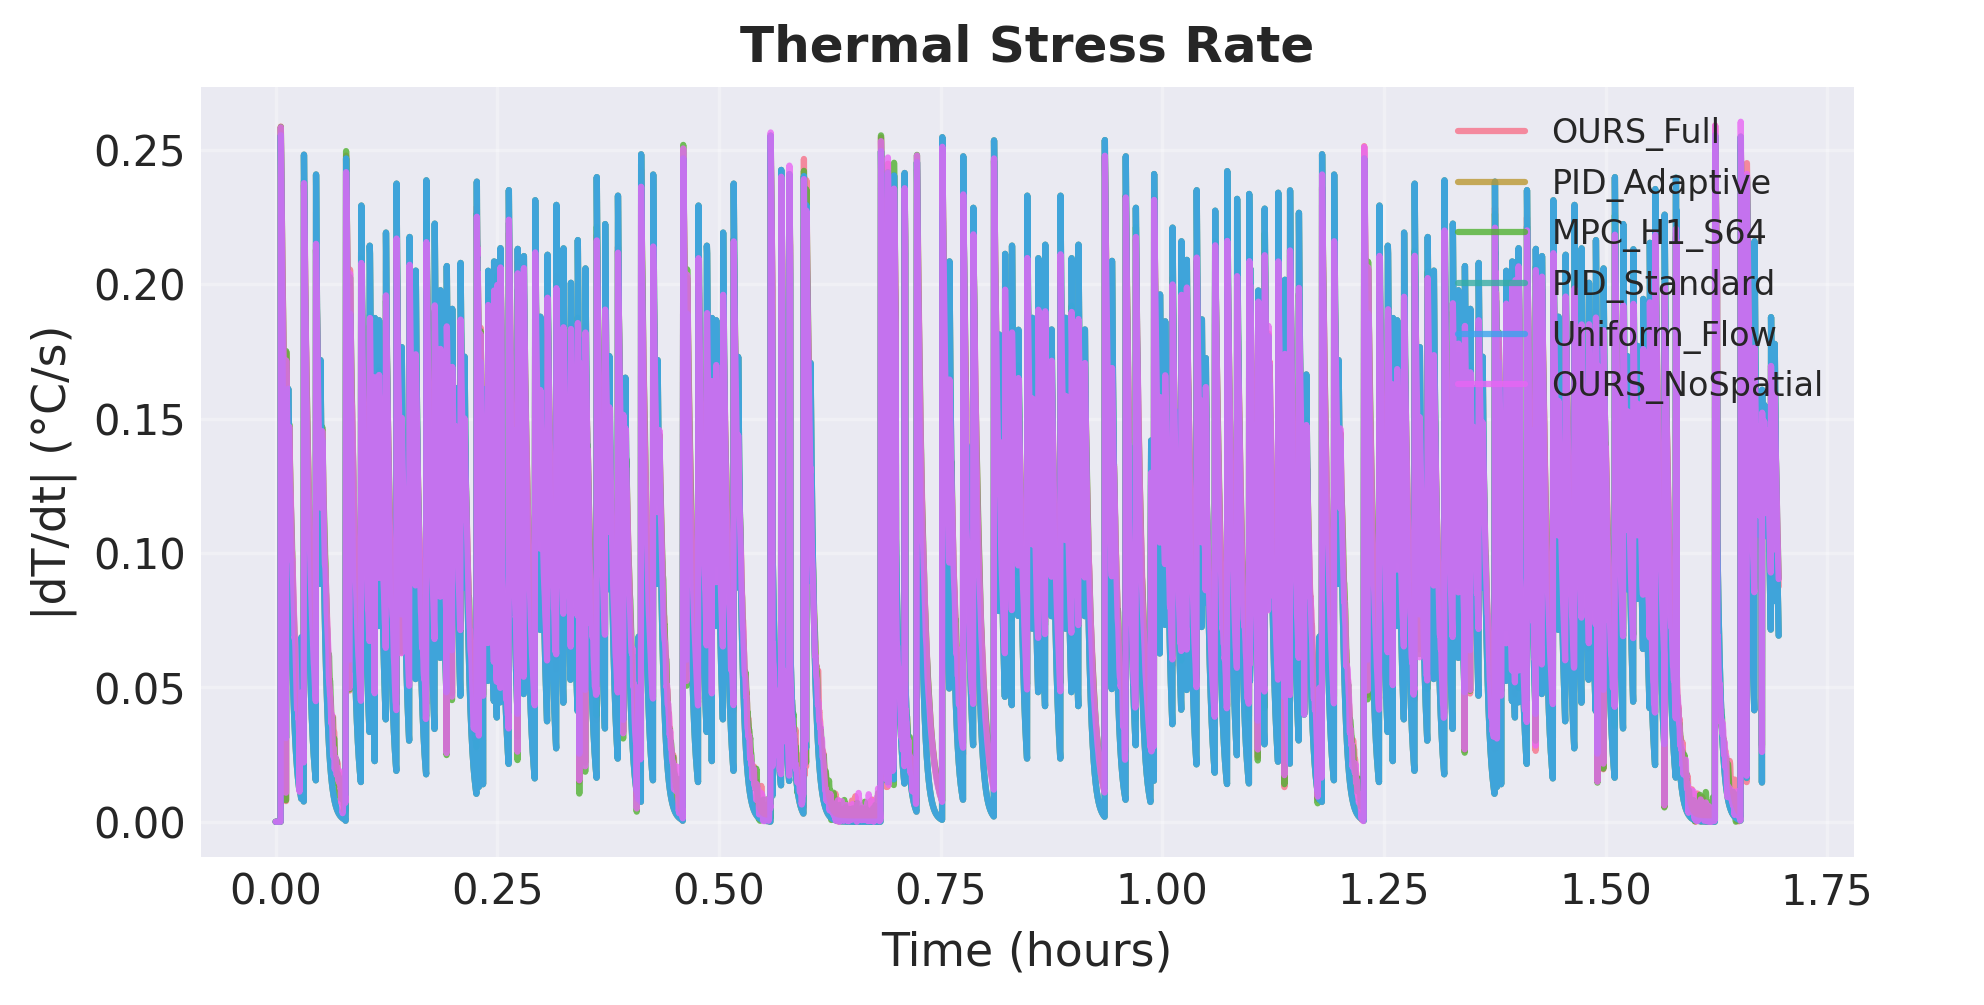
\includegraphics[width=0.8\linewidth]{analysis_temporal_dashboard_r3c1.png}
    \caption{Temporal panel five. Thermal stress rate evolution.}
    \label{fig:temporal_r3c1}
\end{figure}

\begin{figure}[htbp]
    \centering
    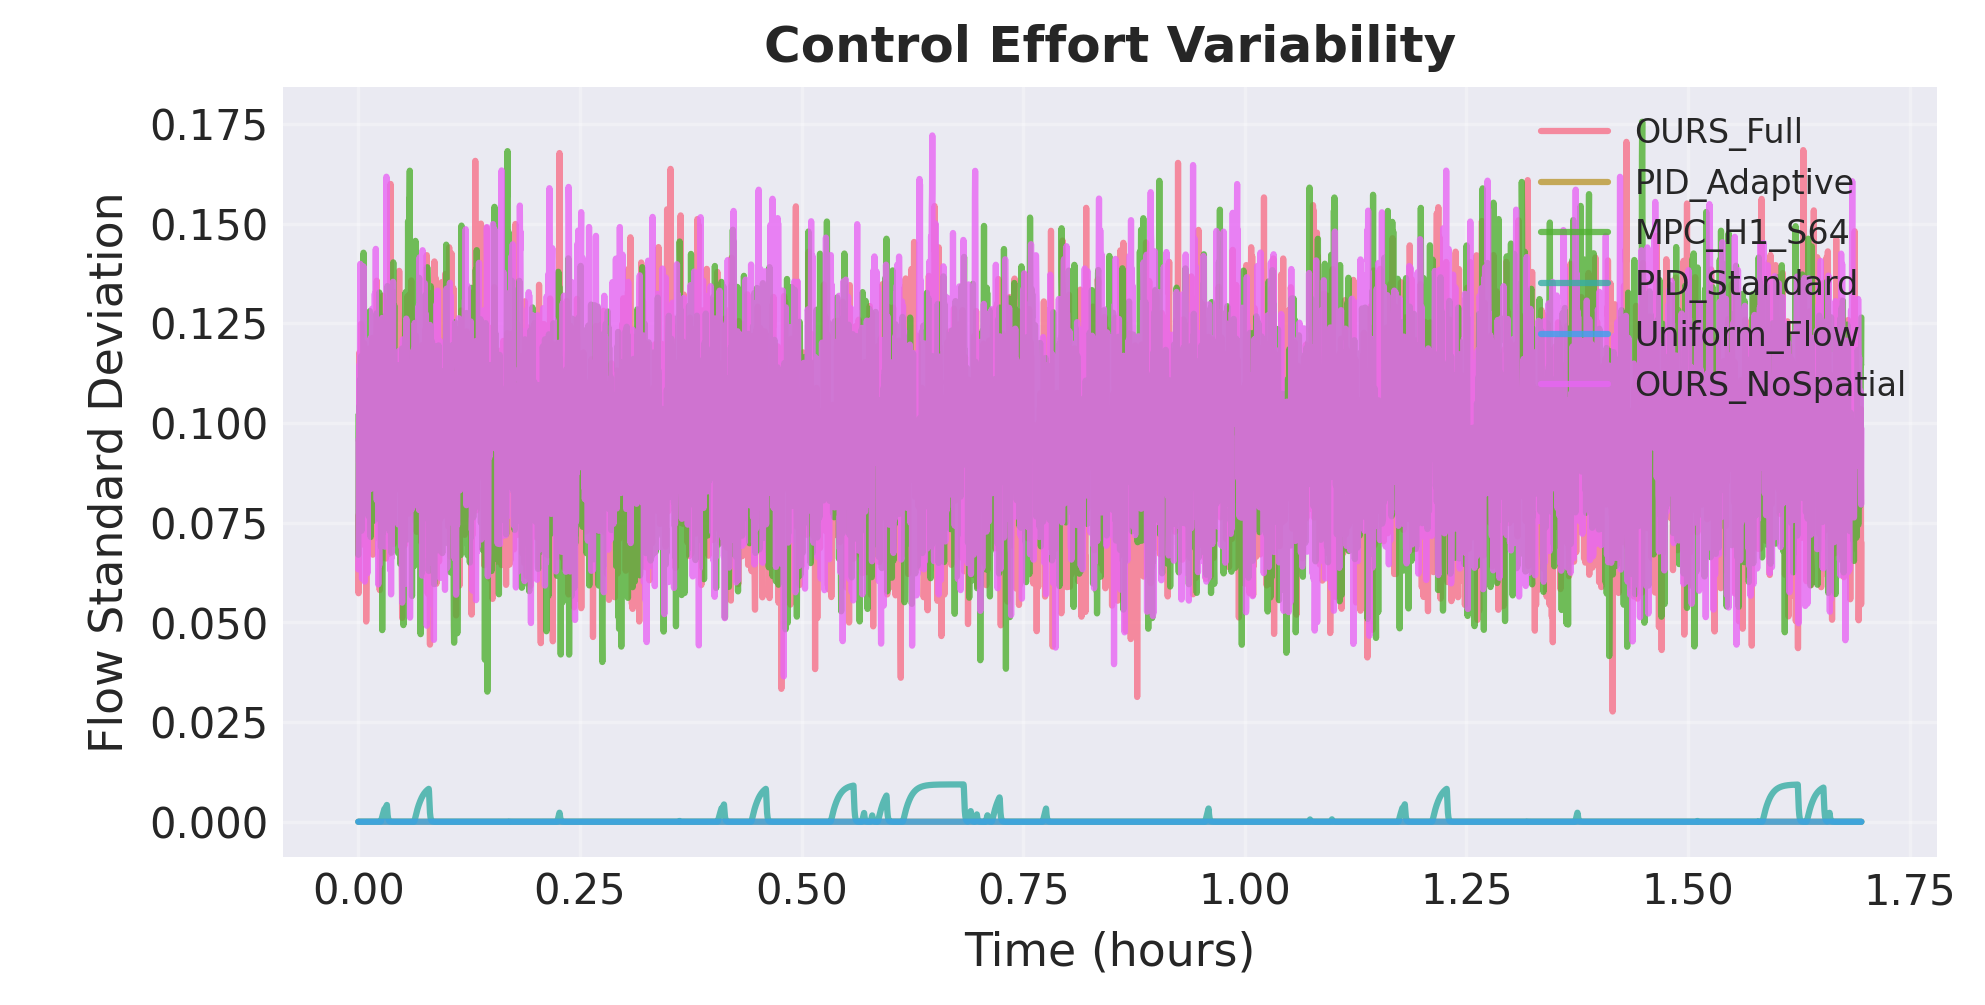
\includegraphics[width=0.8\linewidth]{analysis_temporal_dashboard_r3c2.png}
    \caption{Temporal panel six. Control effort variability over time.}
    \label{fig:temporal_r3c2}
\end{figure}

\paragraph{Thermal stress and effort variability}
Figures \ref{fig:temporal_r3c1} and \ref{fig:temporal_r3c2} examine stress and command variability patterns.
Thermal stress rate captures abrupt temperature changes that influence material fatigue risk.
Predictive methods maintain moderate stress with fewer sharp transients over time.
Proportional control also limits stress during most operating windows.
PID methods show stronger stress events during aggressive correction phases.
Variability trends mirror this behavior across the compared controller families.
Predictive policies change commands smoothly with less erratic switching behavior.
Lower switching frequency reduces mechanical wear in valves and pumping equipment.
PID policies exhibit larger command swings and frequent corrective oscillation episodes.
These panels connect algorithm behavior with durability and maintenance implications.
They support selecting smoother policies for long service life requirements. Smoother behavior often correlates with lower maintenance demand over fleet operation. Reduced switching also lowers noise and improves perceived system quality. Reliability gains can offset modest temperature compromises in some applications. These insights add lifecycle value to controller selection decisions.

\subsubsection{Statistical behavior analysis}

\begin{figure}[htbp]
    \centering
    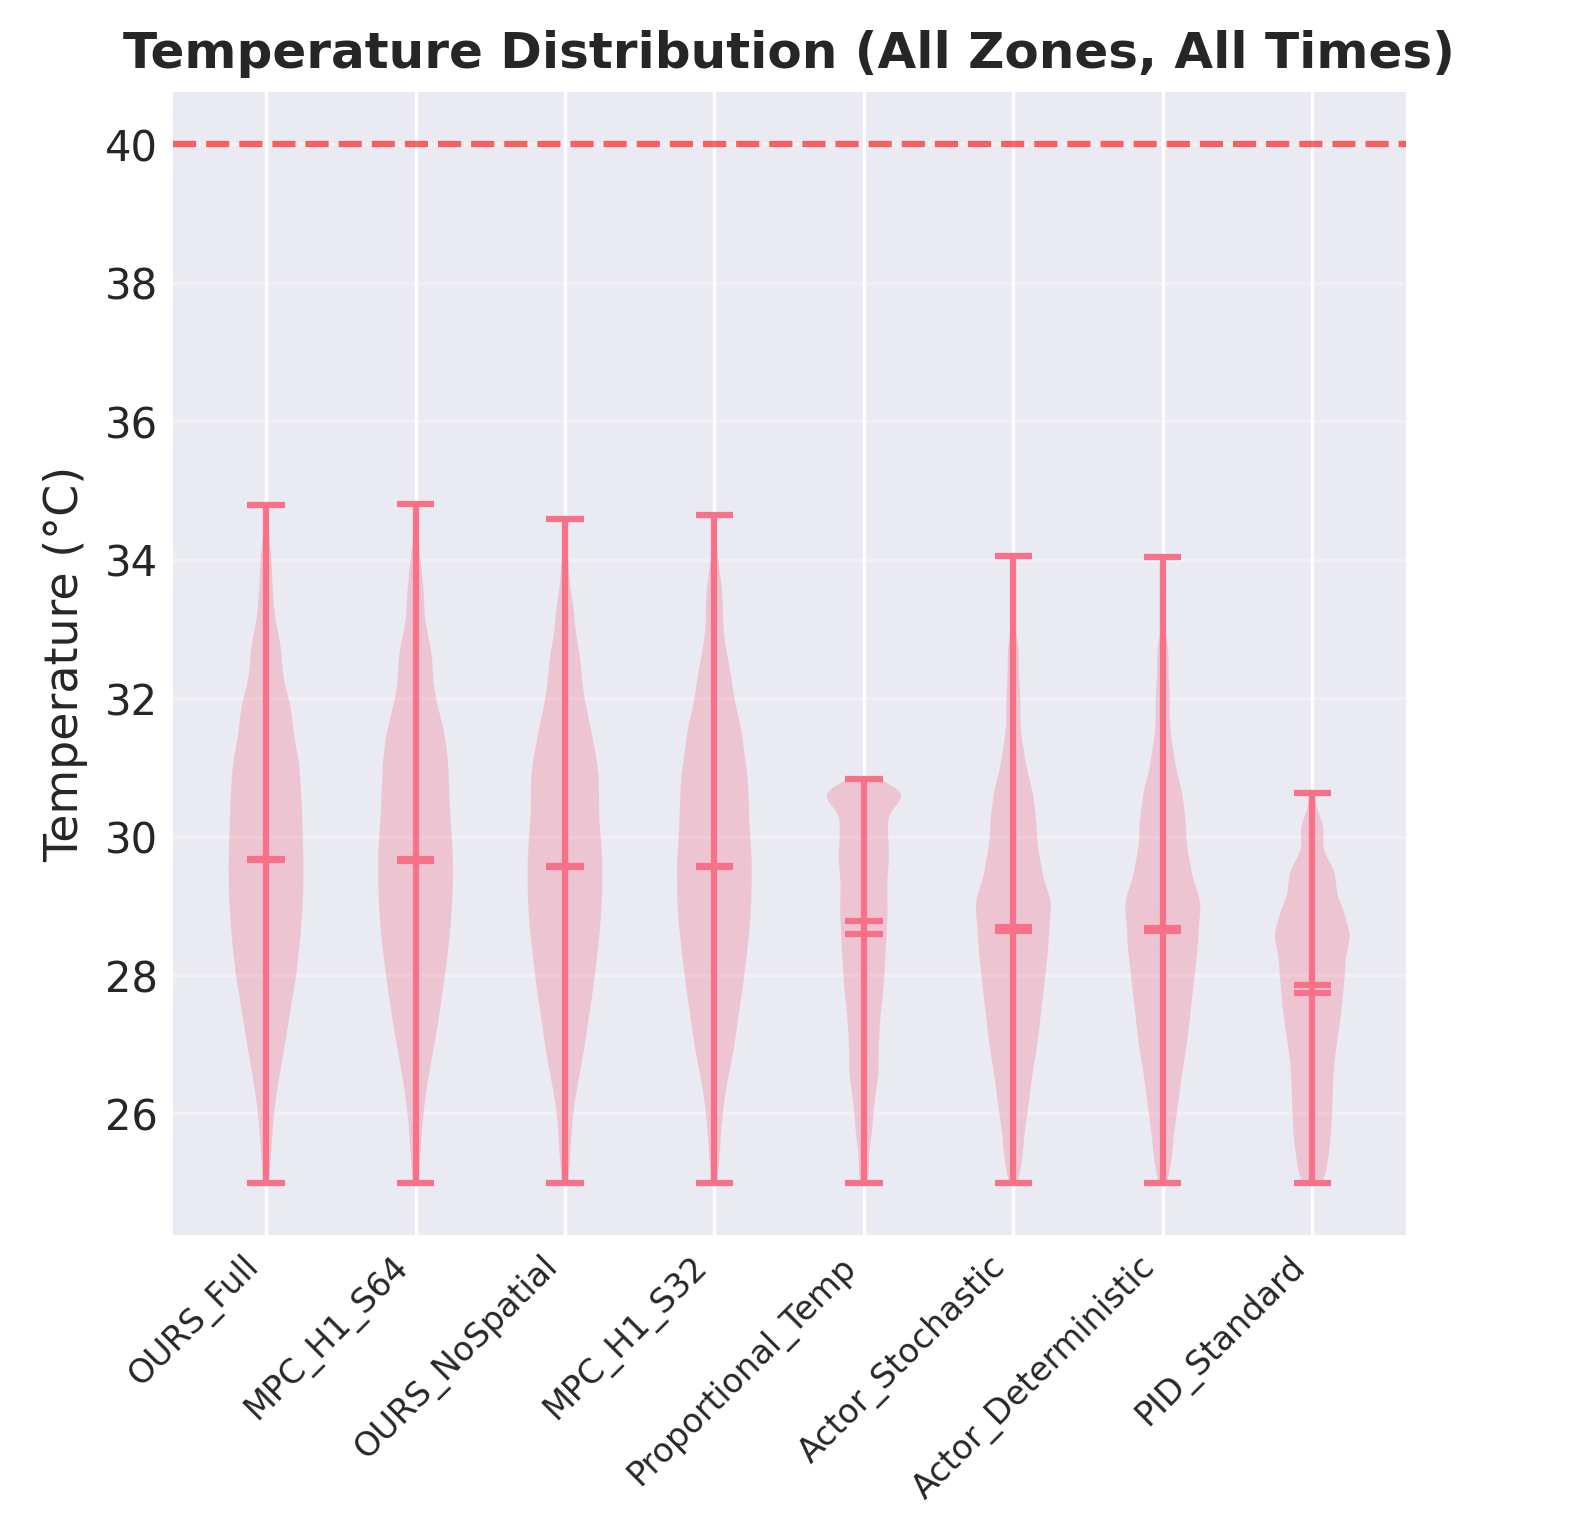
\includegraphics[width=0.8\linewidth]{analysis_statistical_distributions_r1c1.png}
    \caption{Statistical panel one. Temperature distribution violin plot.}
    \label{fig:stats_r1c1}
\end{figure}

\begin{figure}[htbp]
    \centering
    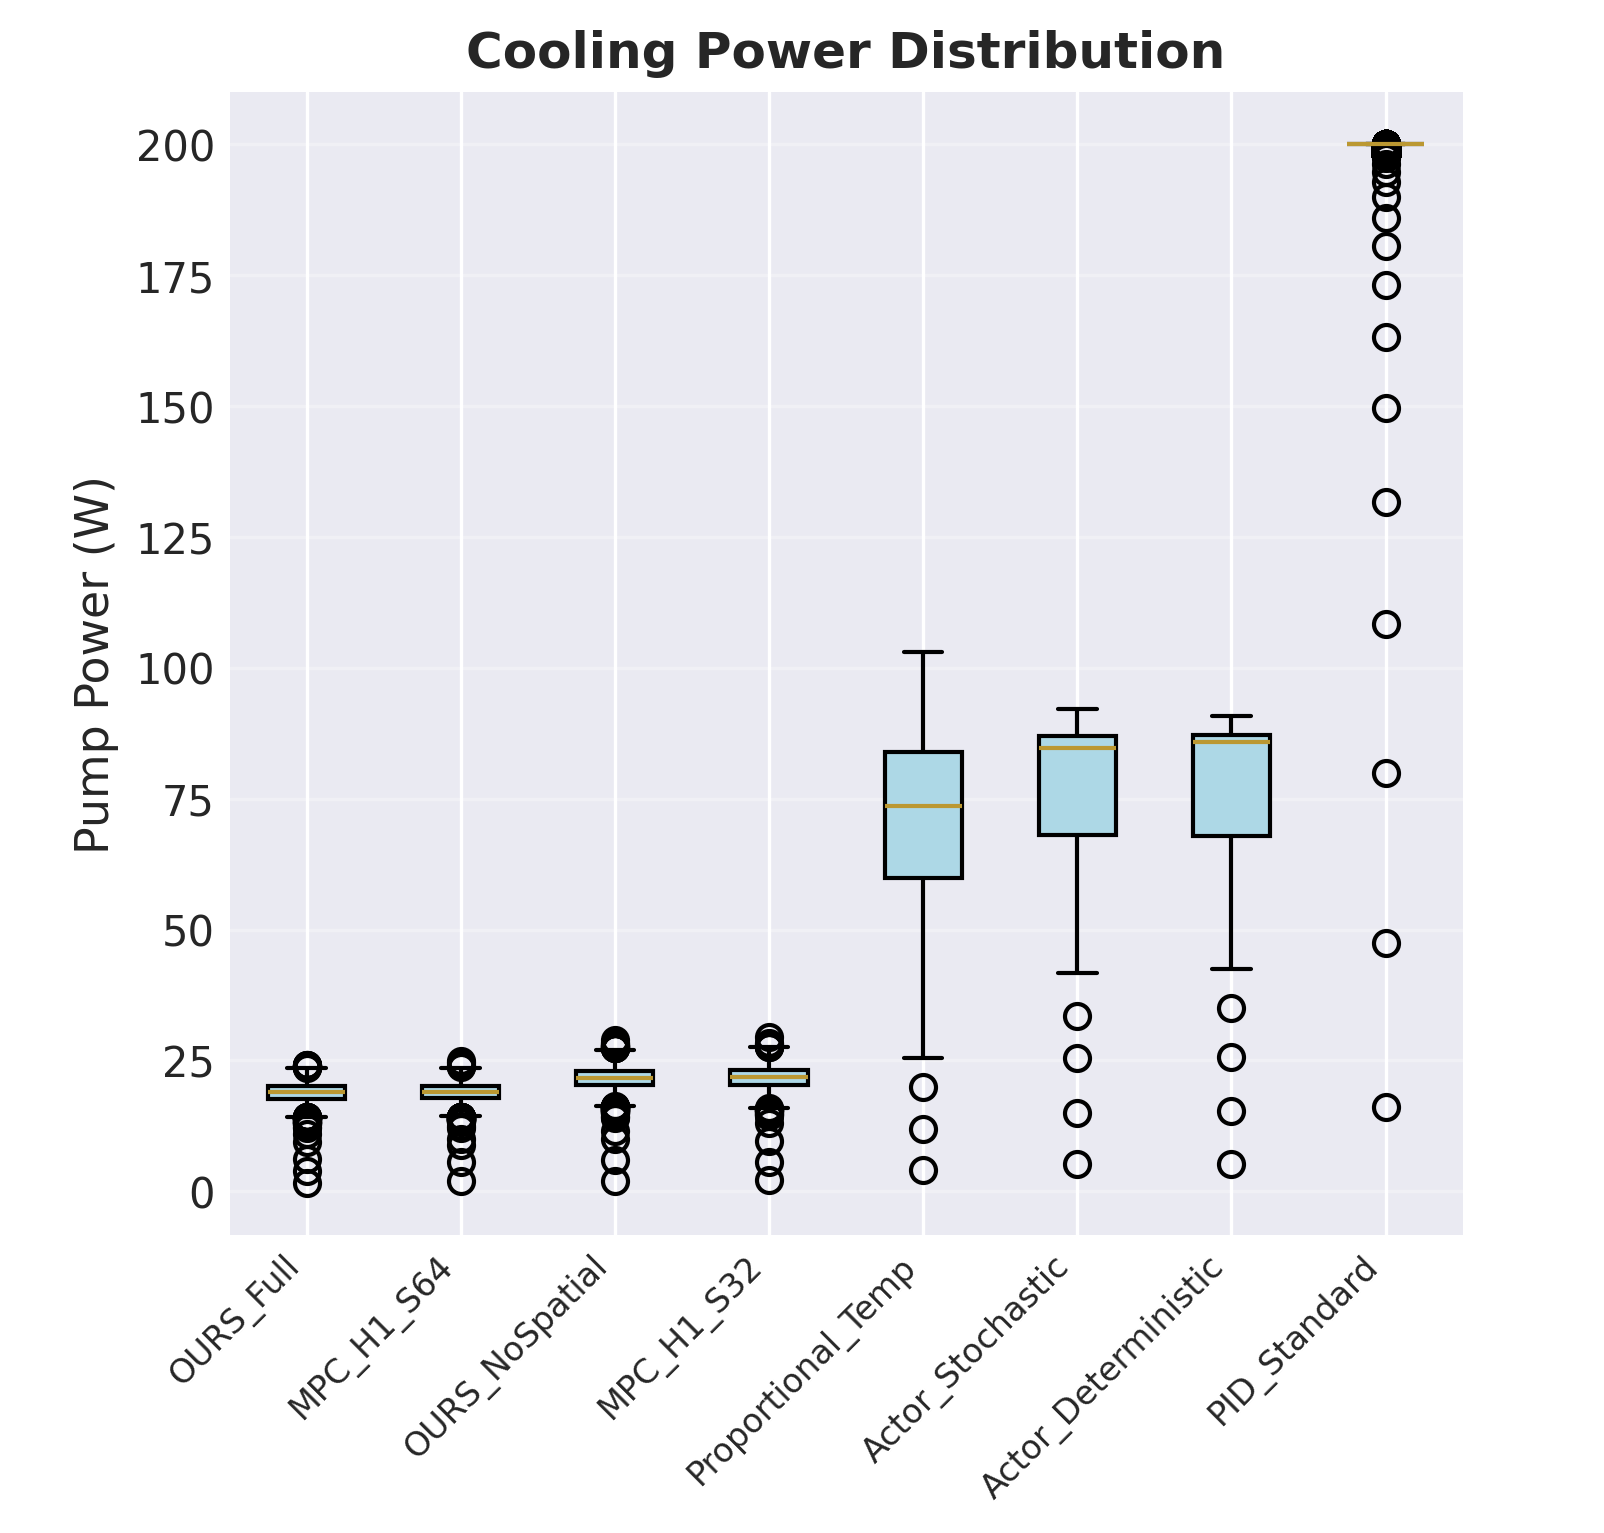
\includegraphics[width=0.8\linewidth]{analysis_statistical_distributions_r1c2.png}
    \caption{Statistical panel two. Cooling power distribution box plot.}
    \label{fig:stats_r1c2}
\end{figure}

\paragraph{Temperature and cooling power distributions}
Figures \ref{fig:stats_r1c1} and \ref{fig:stats_r1c2} summarize temperature and power distribution structure.
Violin width indicates variability across zones, time, and operating modes.
Proportional control shows concentrated temperature mass with relatively narrow tails.
Predictive methods show slightly wider distributions with controlled extreme values.
PID methods show broader distributions during sustained conservative cooling intervals.
Power box plots reveal typical demand through medians and quartile spread.
PID methods show higher medians and longer upper whisker behavior.
Predictive methods maintain lower central demand and fewer extreme power events.
These observations align with cumulative energy patterns from temporal analysis.
Distribution views confirm differences are structural, not isolated transient incidents.
The pair strengthens confidence in efficiency conclusions across controller groups. Distribution consistency indicates results are not driven by isolated outlier events. Central tendencies and tails both support the same ordering trends. This agreement improves statistical credibility for comparative claims. It also supports robust interpretation across varying operational contexts. This consistency strengthens confidence when extending conclusions across different mission profiles.

\begin{figure}[htbp]
    \centering
    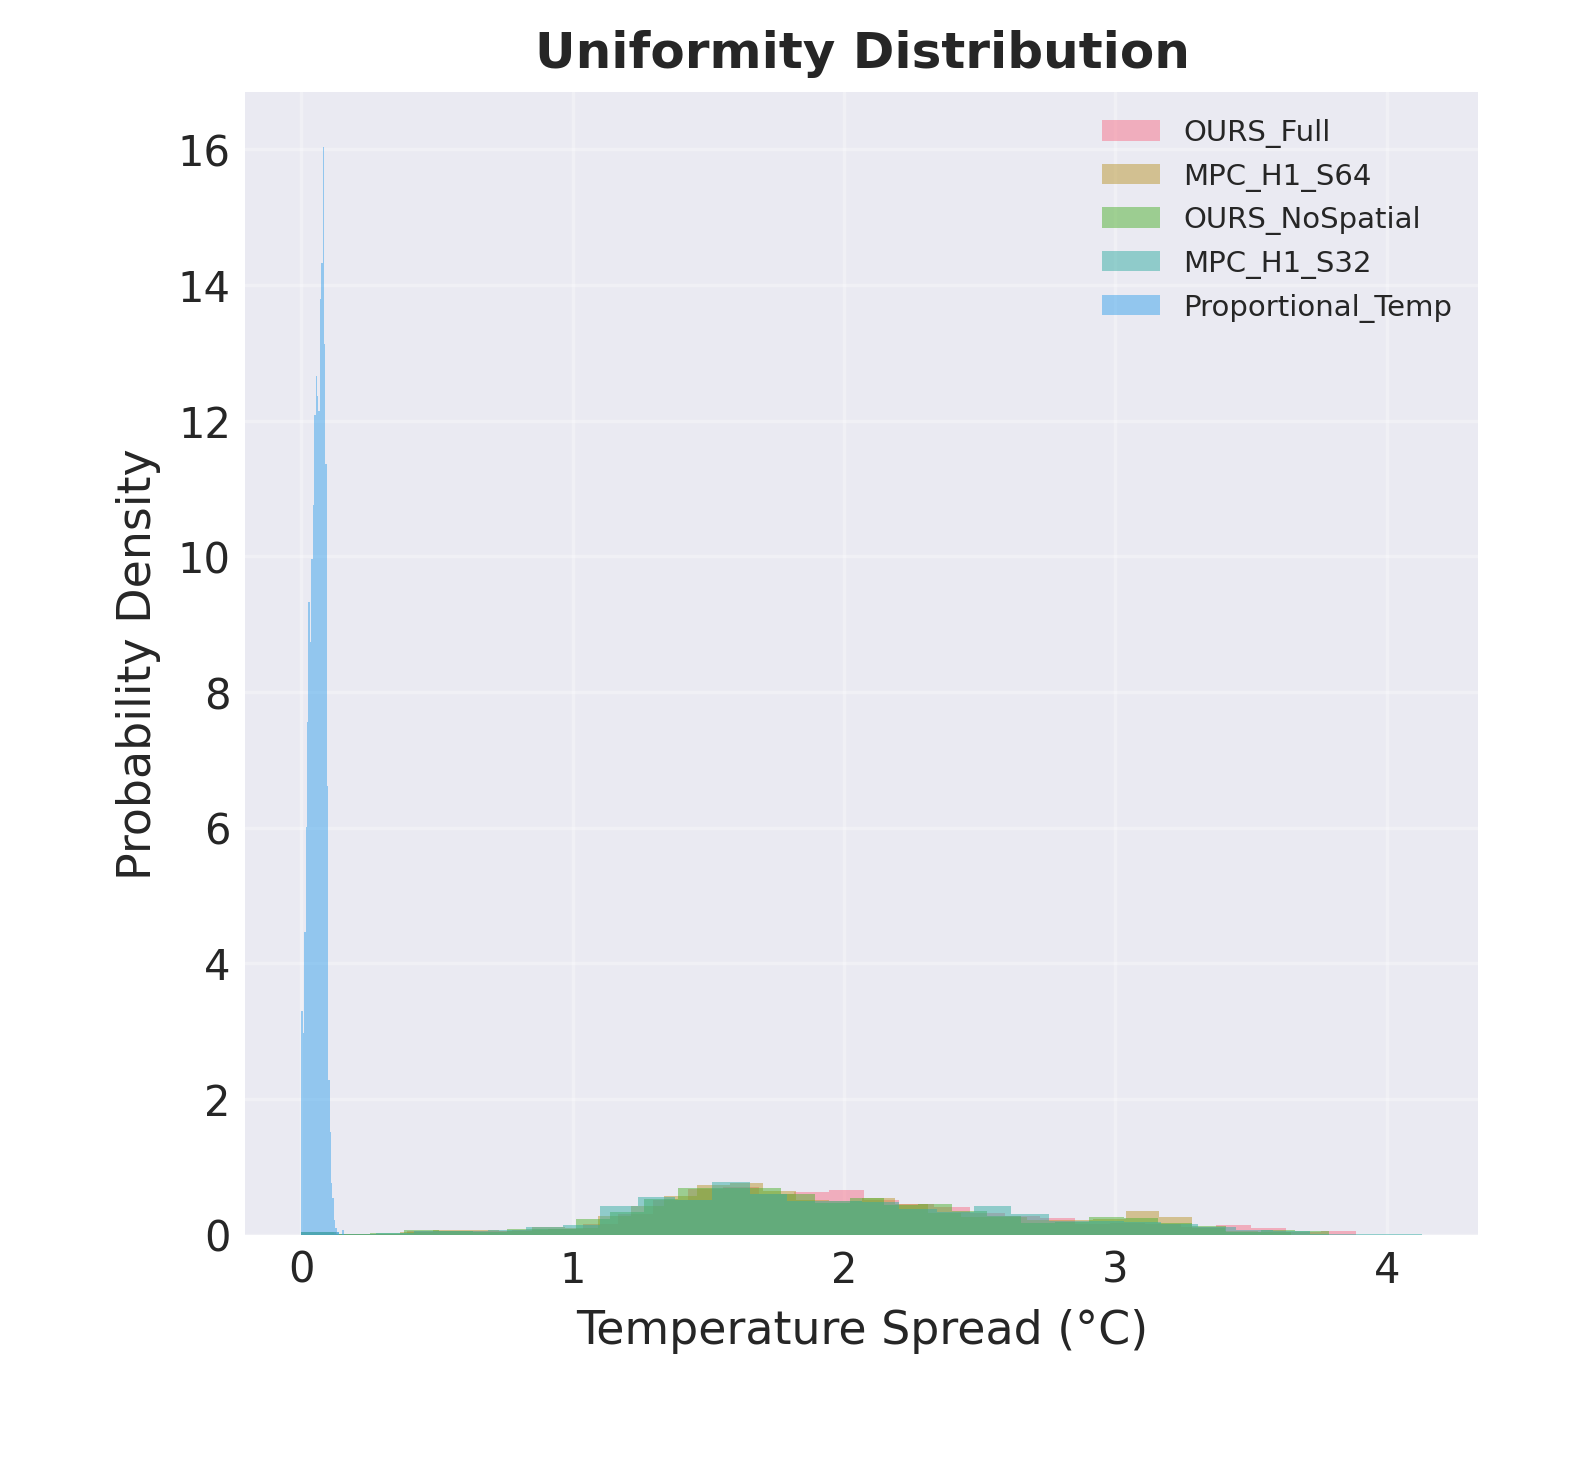
\includegraphics[width=0.8\linewidth]{analysis_statistical_distributions_r1c3.png}
    \caption{Statistical panel three. Uniformity distribution histogram.}
    \label{fig:stats_r1c3}
\end{figure}

\begin{figure}[htbp]
    \centering
    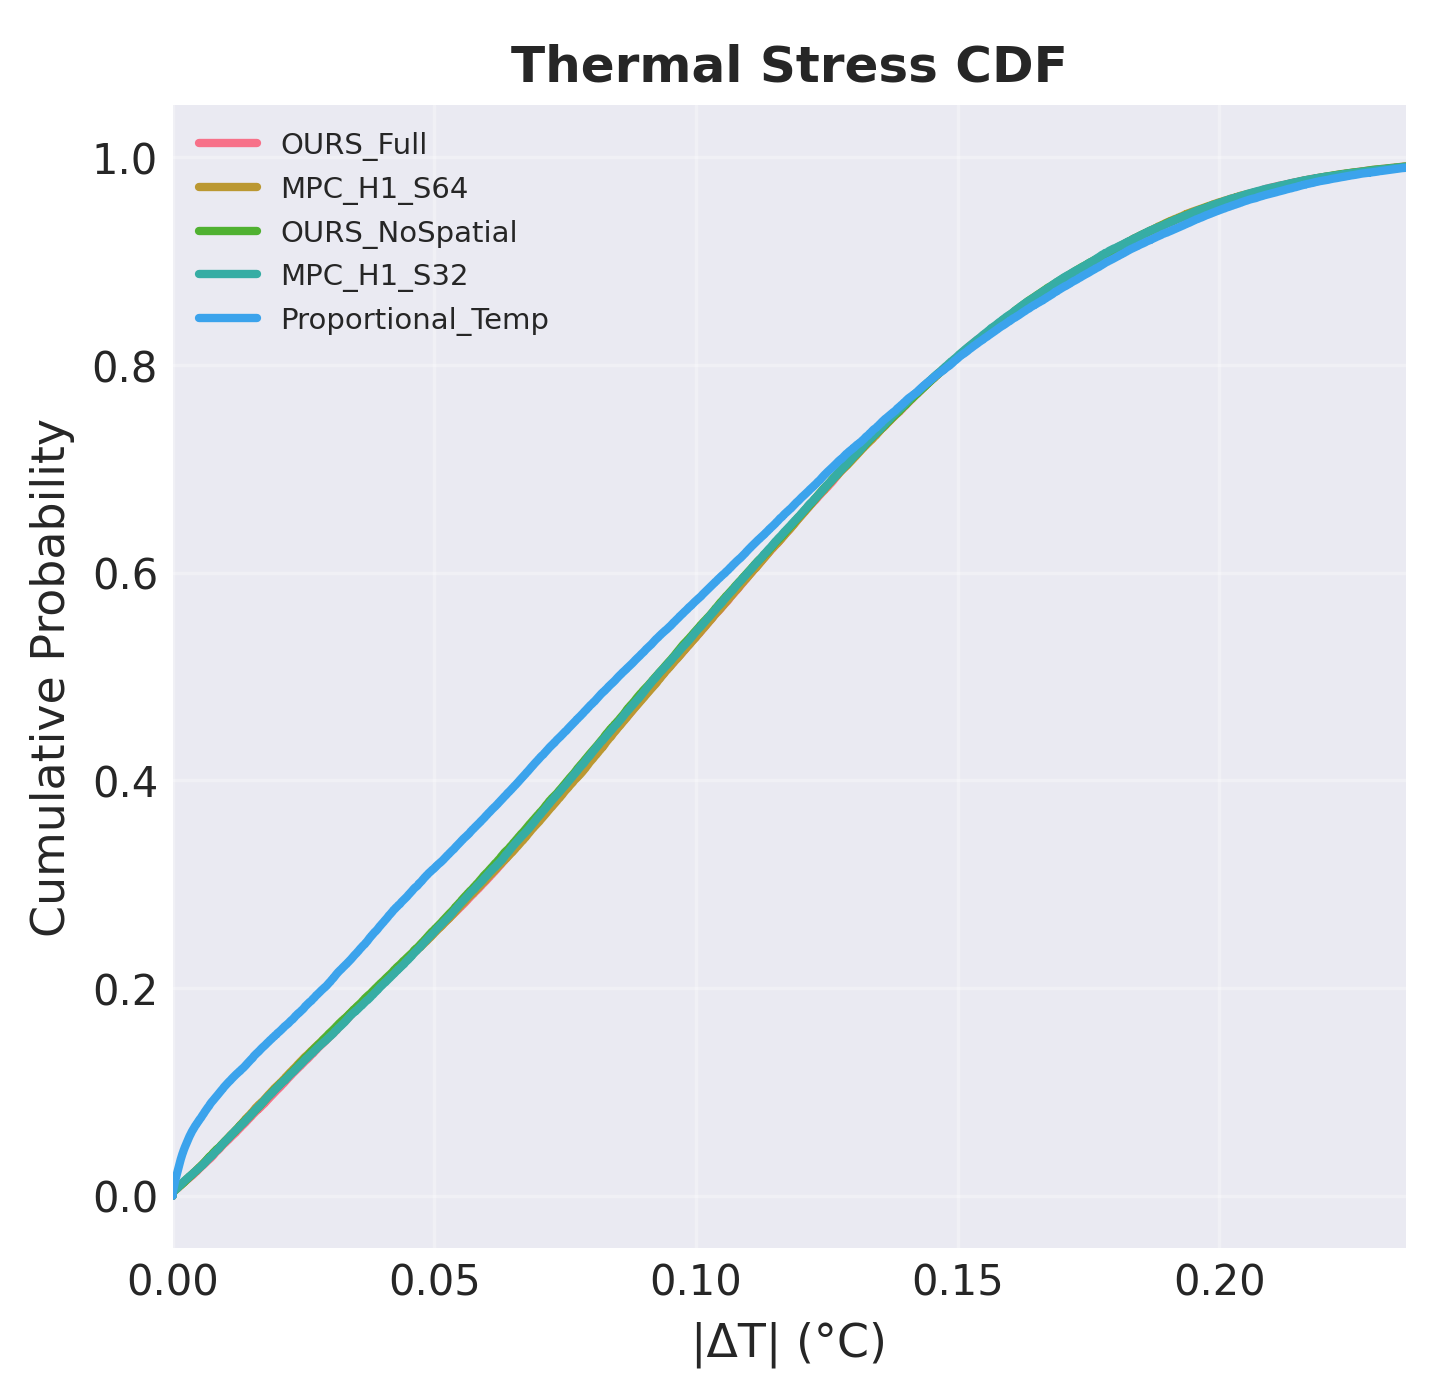
\includegraphics[width=0.8\linewidth]{analysis_statistical_distributions_r2c1.png}
    \caption{Statistical panel four. Thermal stress cumulative distribution.}
    \label{fig:stats_r2c1}
\end{figure}

\paragraph{Uniformity and stress distributions}
Figures \ref{fig:stats_r1c3} and \ref{fig:stats_r2c1} characterize spread and stress probability behavior.
Histogram mass near lower spread indicates stronger pack uniformity performance.
Proportional control places most probability in low spread regions.
Predictive methods shift moderate probability toward slightly larger spread intervals.
This shift reflects targeted cooling decisions under energy constrained operation.
Stress cumulative curves indicate predictive methods favor lower stress probability.
PID curves place more mass in higher stress regions during correction episodes.
Higher stress probability can increase long term degradation risk across components.
Together these plots quantify reliability relevant consequences of policy differences.
They also support threshold based tuning for allowable spread and stress levels.
This pair adds risk centered evidence beyond simple average metrics. Rare events often determine safety outcomes in thermal management systems. Probability views reveal those events more clearly than mean values. Risk aware interpretation improves threshold definition for practical deployment. The evidence therefore supports safer controller tuning under uncertainty.

\begin{figure}[htbp]
    \centering
    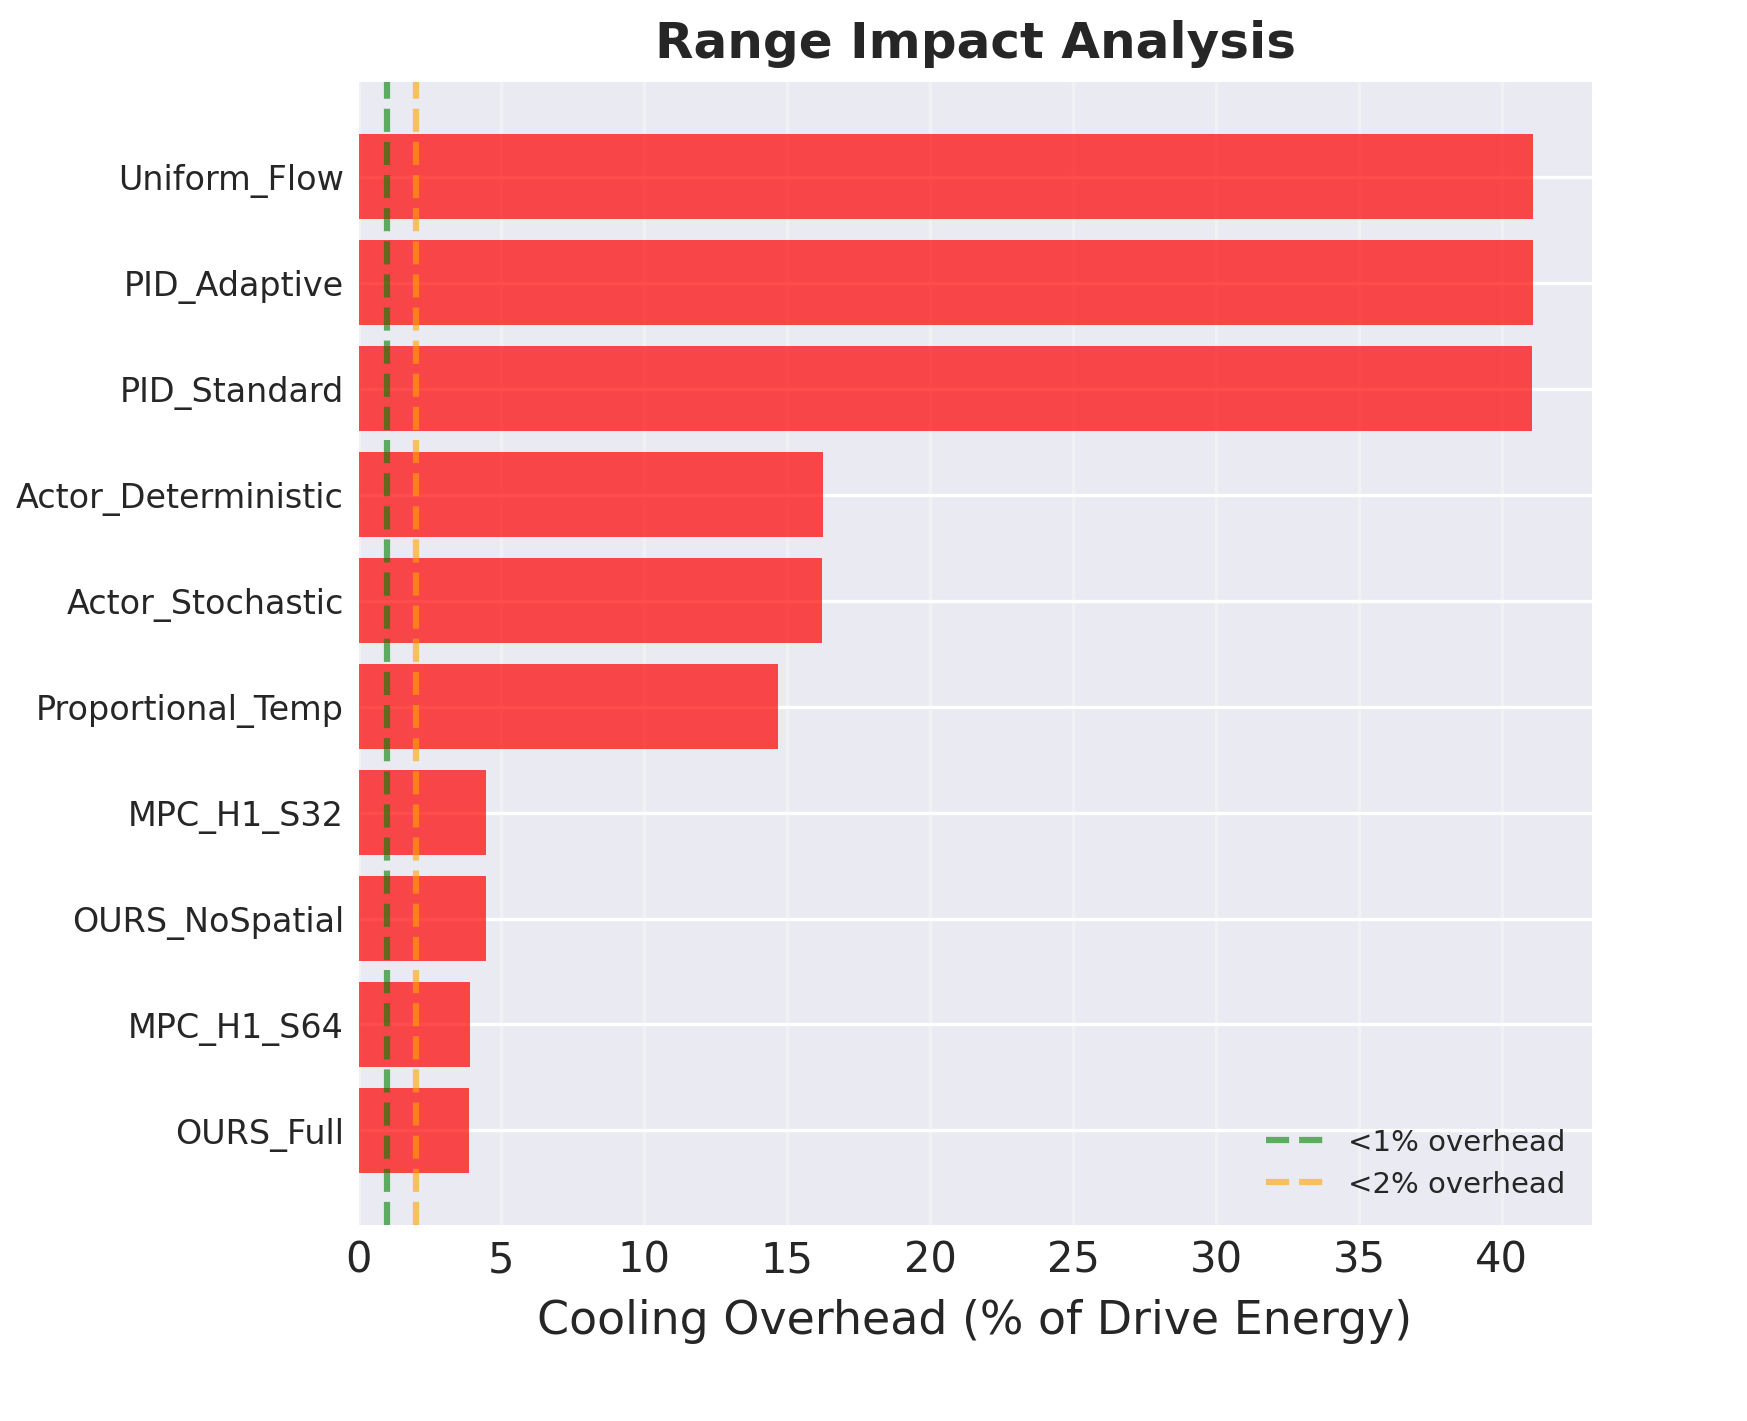
\includegraphics[width=0.8\linewidth]{analysis_statistical_distributions_r2c2.png}
    \caption{Statistical panel five. Cooling overhead comparison.}
    \label{fig:stats_r2c2}
\end{figure}

\begin{figure}[htbp]
    \centering
    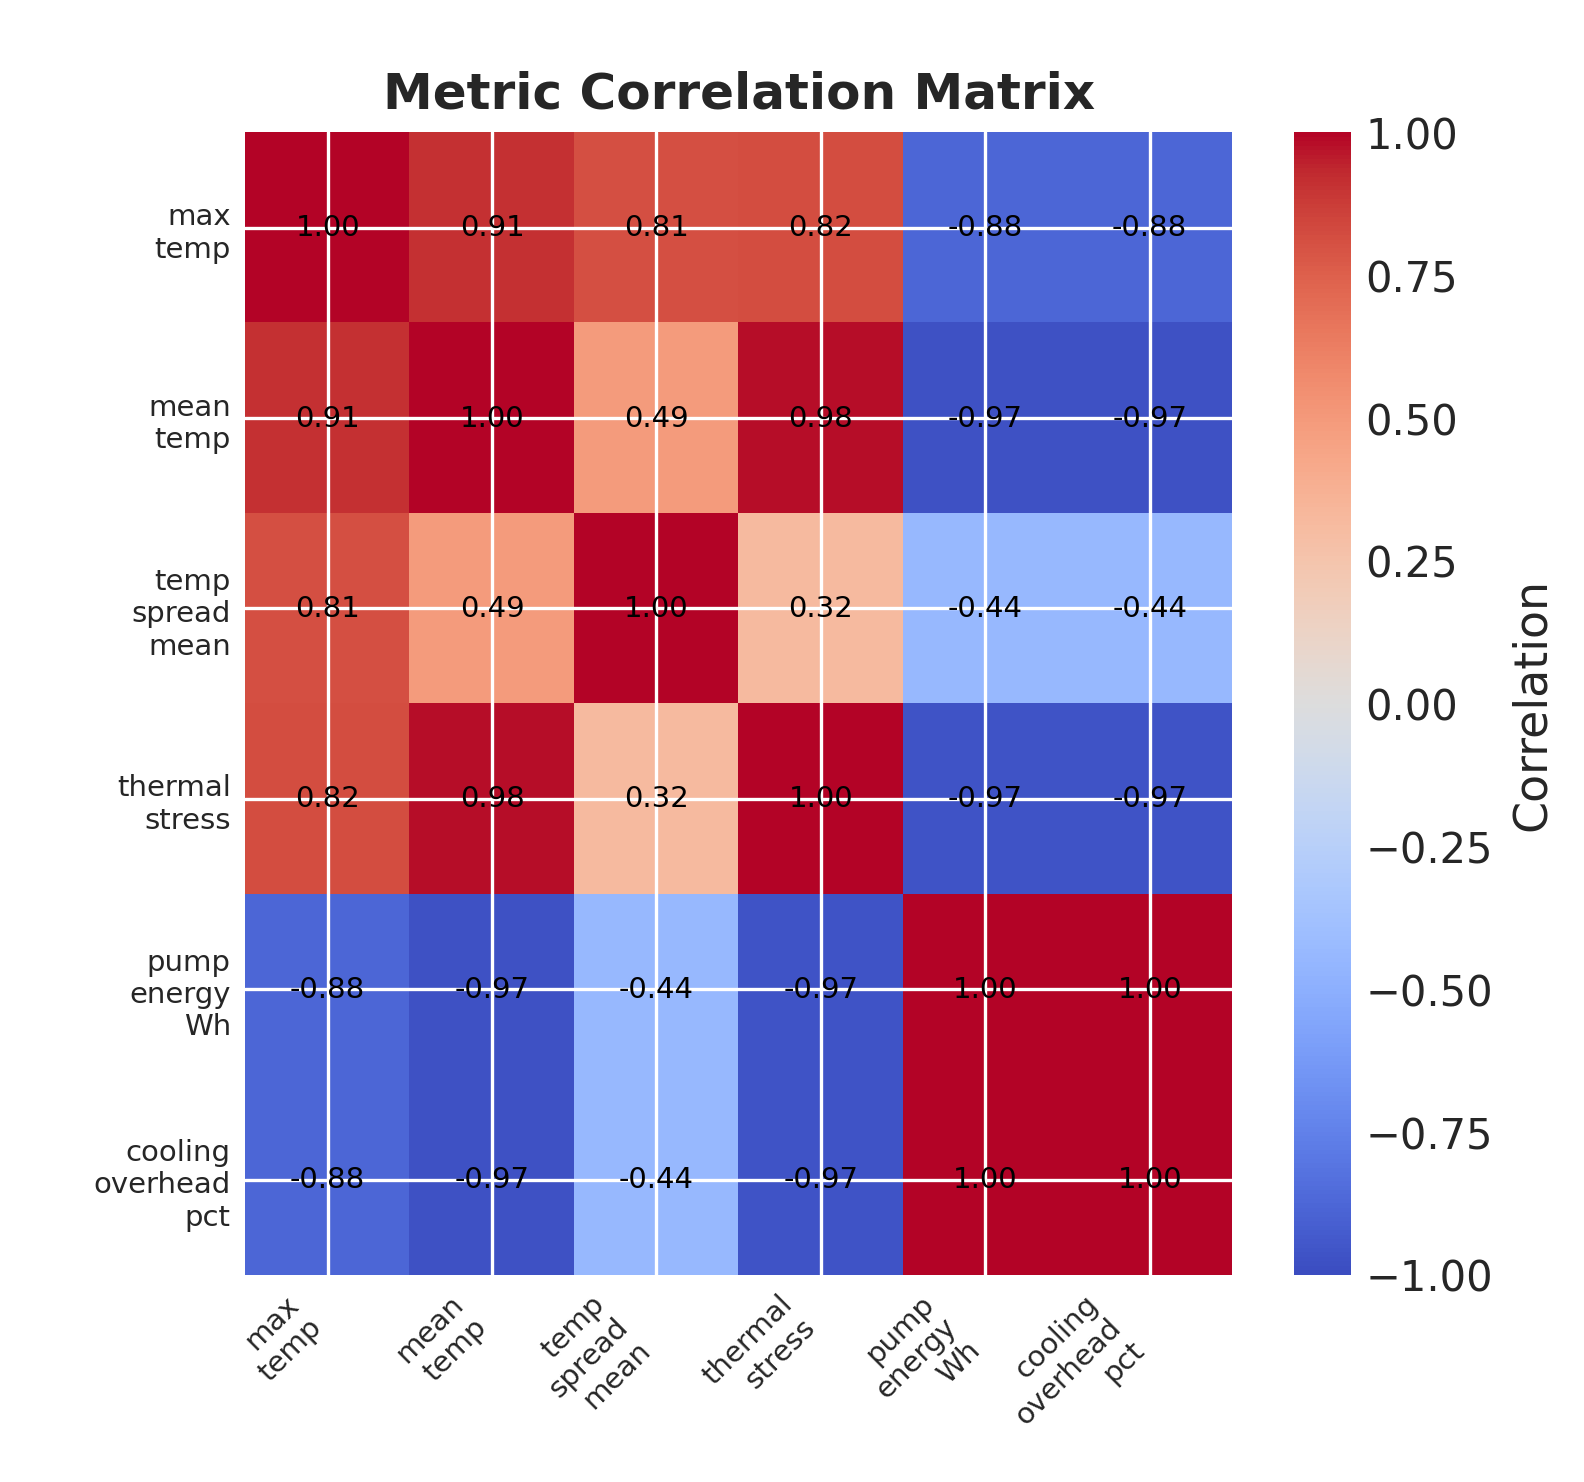
\includegraphics[width=0.8\linewidth]{analysis_statistical_distributions_r2c3.png}
    \caption{Statistical panel six. Metric correlation heatmap.}
    \label{fig:stats_r2c3}
\end{figure}

\paragraph{Overhead and metric coupling}
Figures \ref{fig:stats_r2c2} and \ref{fig:stats_r2c3} connect overhead magnitude with metric relationships.
Overhead values compare auxiliary cooling demand against propulsion energy requirement.
Predictive methods report lower overhead than conservative PID alternatives.
OURS Full and MPC variants remain near the most efficient overhead values.
Correlation patterns show strong linkage between cooling energy and overhead metrics.
Spread and stress also show meaningful association in several control regimes.
These couplings confirm objectives cannot be optimized independently without consequences.
Design decisions must balance safety, uniformity, and efficiency simultaneously.
The heatmap clarifies which trade pairs deserve priority during tuning.
Overhead bars translate those trade patterns into mission level energy impact.
This pair therefore anchors multi metric decision making for deployment. Coupled metrics require explicit compromise rather than isolated optimization. Decision makers can prioritize objectives using clear correlation guidance. Overhead values translate abstract trade relations into practical mission impact. This linkage supports accountable and explainable engineering choices. It also clarifies compromises before deployment decisions are finalized by stakeholders.

\subsubsection{Spatial behavior analysis}

\begin{figure}[htbp]
    \centering
    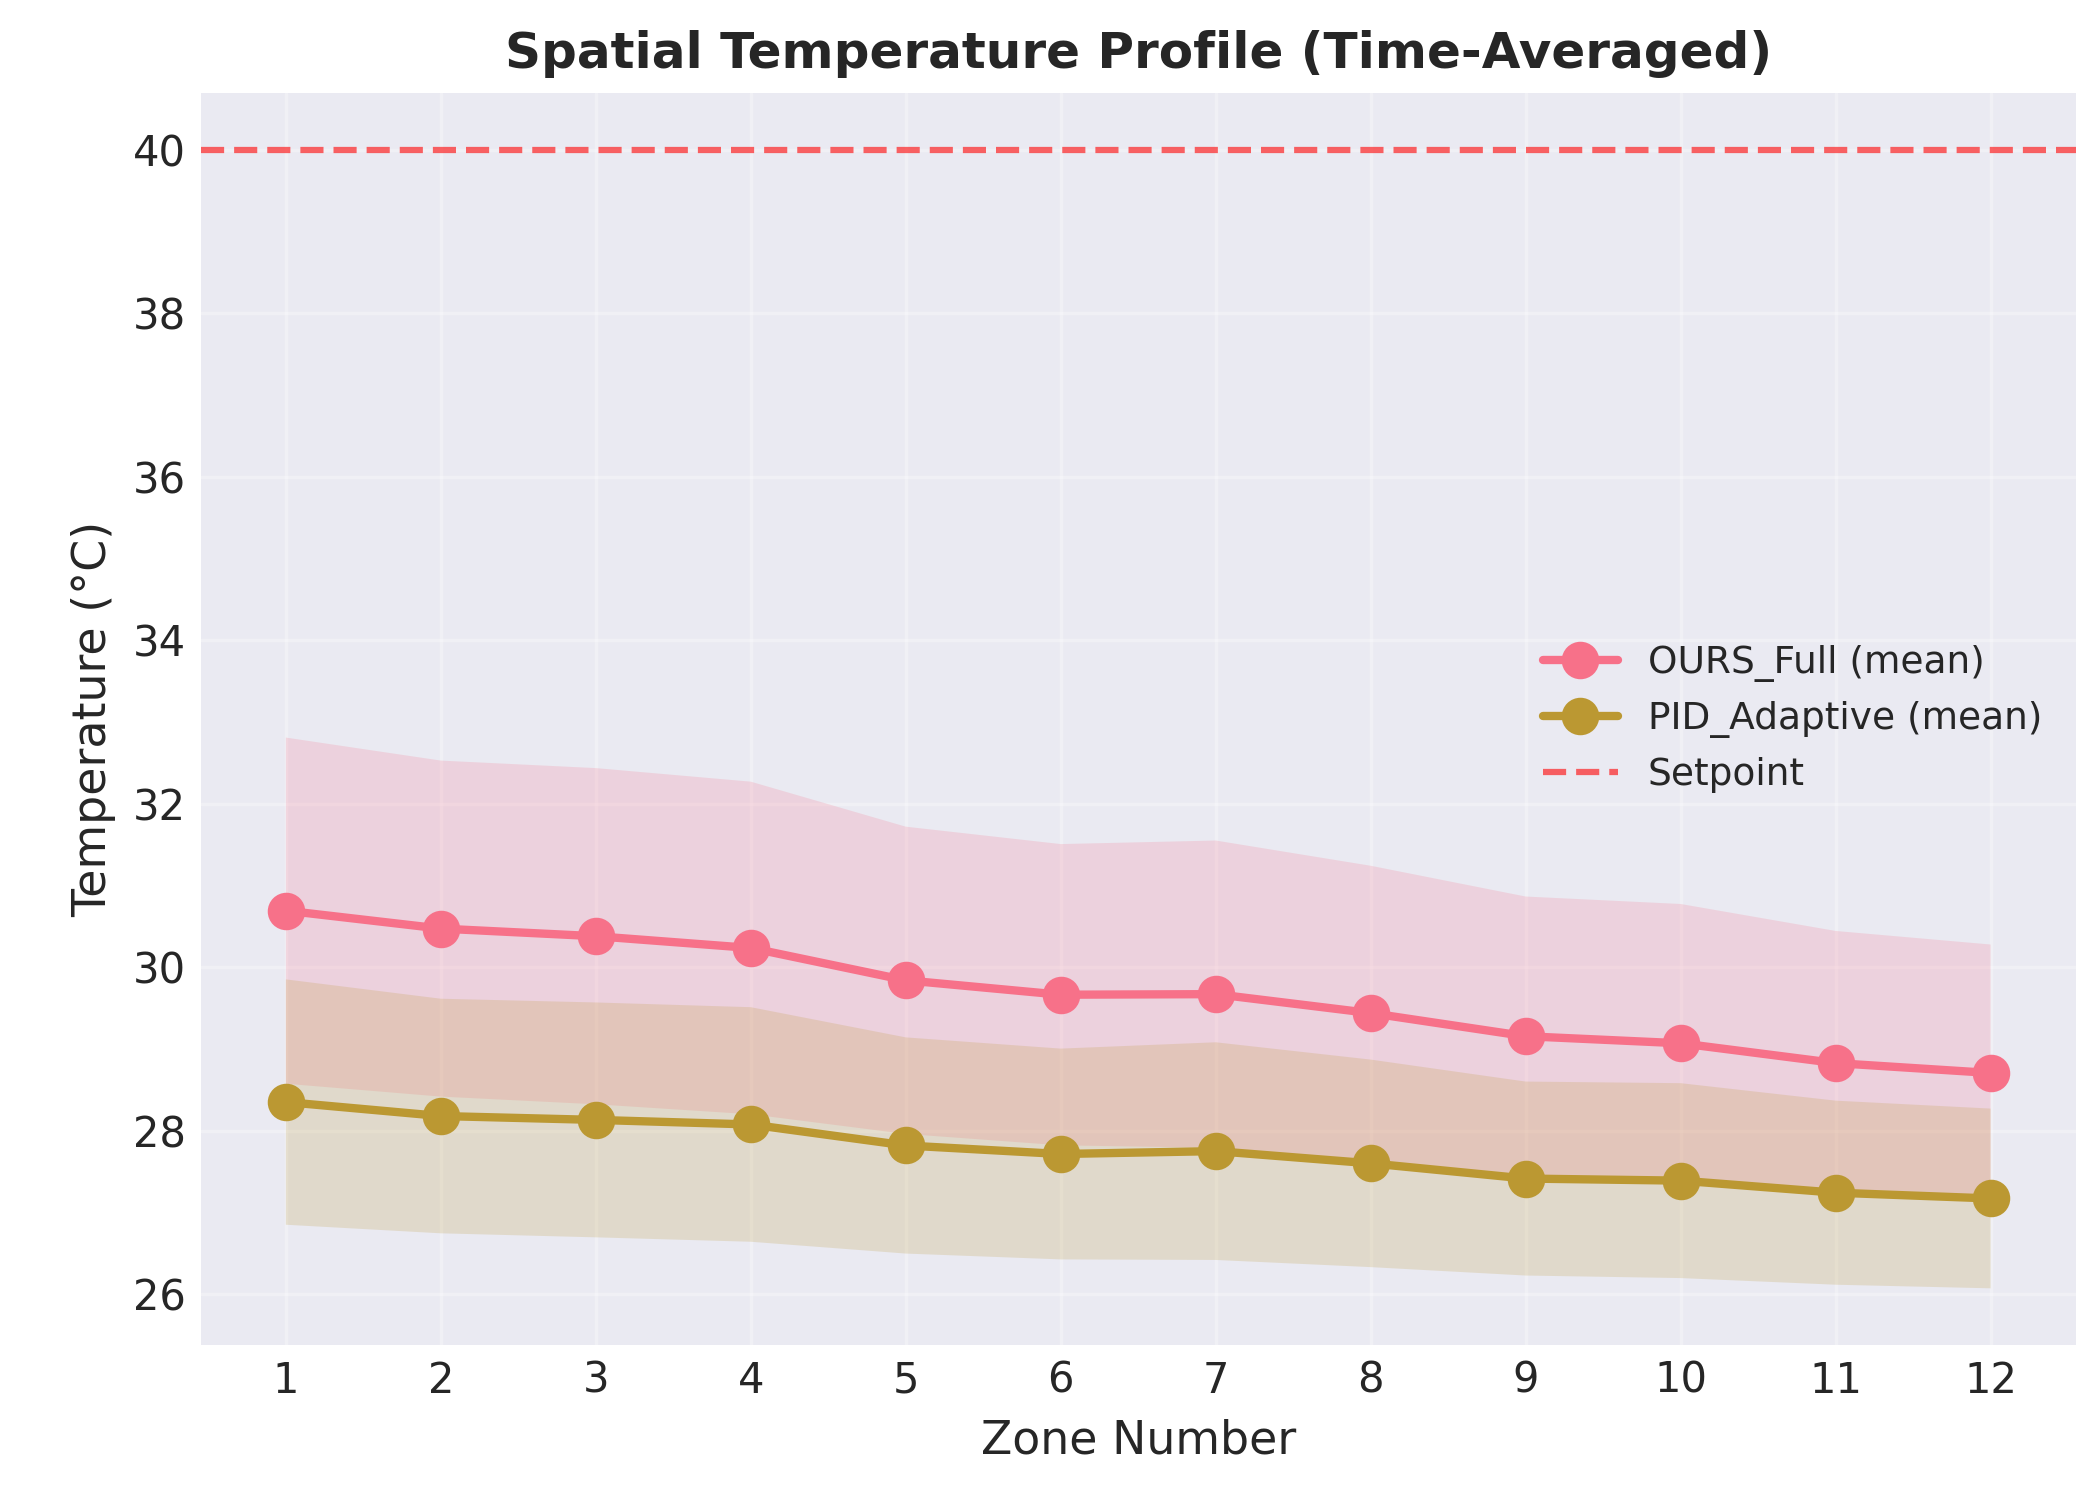
\includegraphics[width=0.8\linewidth]{analysis_spatial_patterns_r1c1.png}
    \caption{Spatial panel one. Time averaged zone temperature profile.}
    \label{fig:spatial_r1c1}
\end{figure}

\begin{figure}[htbp]
    \centering
    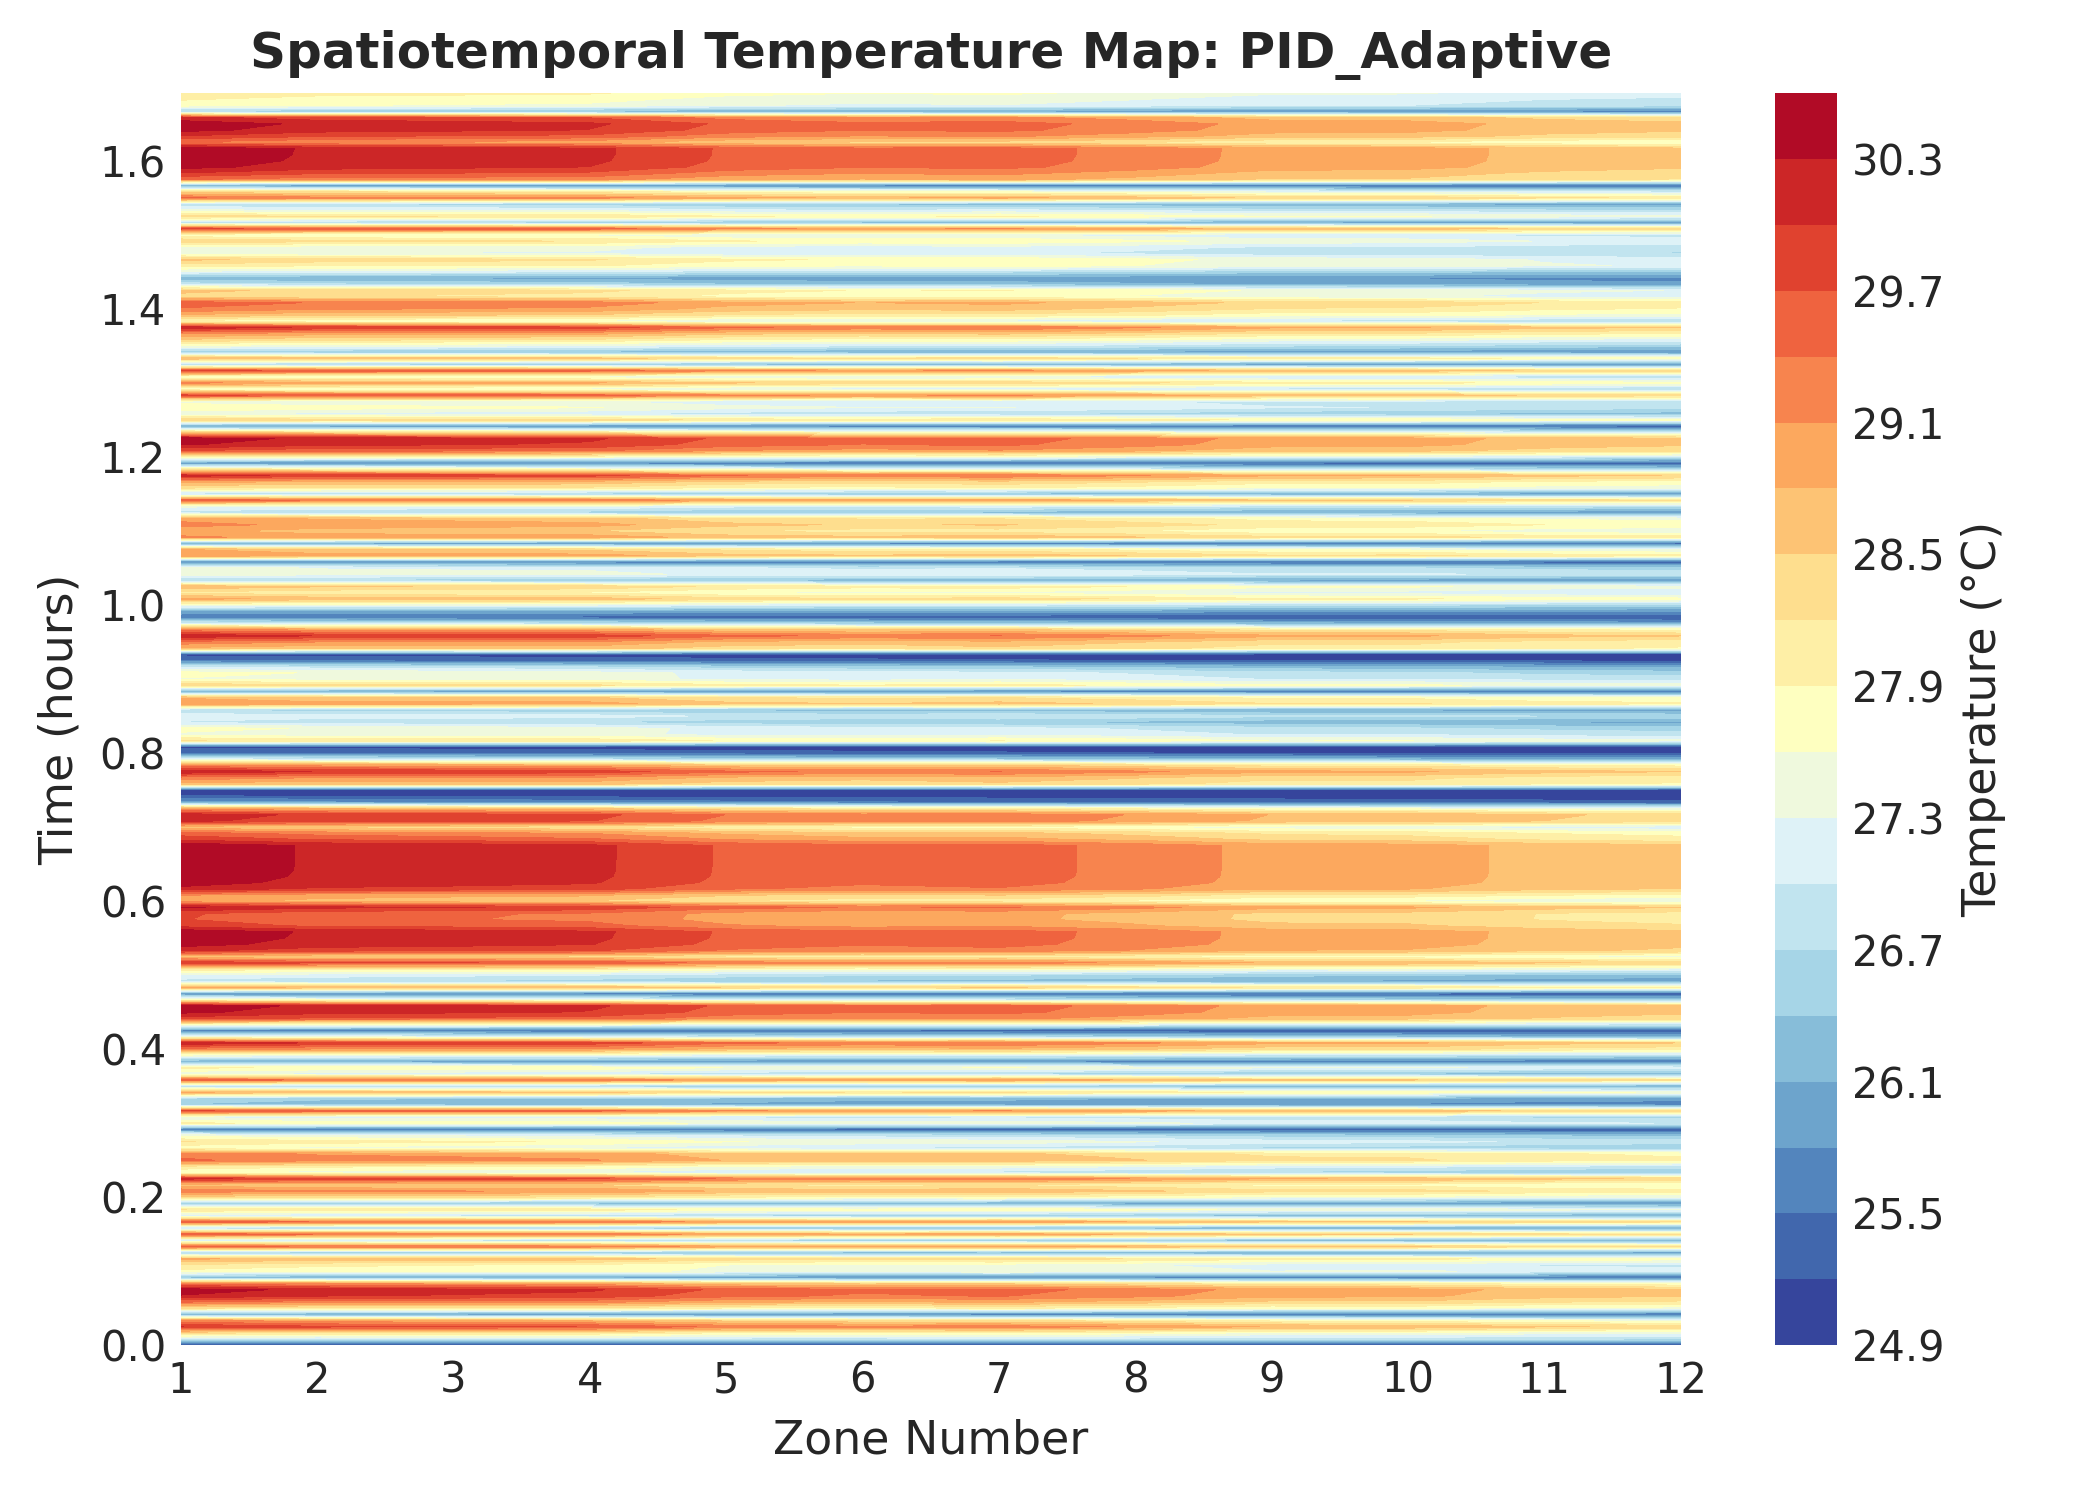
\includegraphics[width=0.8\linewidth]{analysis_spatial_patterns_r1c2.png}
    \caption{Spatial panel two. Temperature gradient comparison.}
    \label{fig:spatial_r1c2}
\end{figure}

\paragraph{Zone profile and gradient}
Figures \ref{fig:spatial_r1c1} and \ref{fig:spatial_r1c2} describe average zone temperatures and gradients.
Profile curves identify persistent warm zones during repeated high demand segments.
Predictive methods lower critical zone means through selective cooling allocation.
Proportional control keeps zone means closely grouped with broader equalized action.
Gradient comparisons show proportional control with consistently low spatial differentials.
Predictive methods allow modest gradients to preserve auxiliary energy.
PID methods reduce gradients through stronger global cooling application.
Global cooling improves uniformity but increases energy and continuous actuator workload.
These patterns explain observed efficiency and spread trade across controllers.
Spatial gradients also indicate potential stress concentration risk in specific zones.
The pair informs sensor density and actuator placement planning decisions. Persistent warm zones suggest where additional sensing can add value. Gradient structure also indicates where actuation authority should increase. Better placement improves control quality without unnecessary hardware expansion. These insights support cost effective pack level architecture planning. They also indicate where hardware upgrades provide the strongest thermal benefit.

\begin{figure}[htbp]
    \centering
    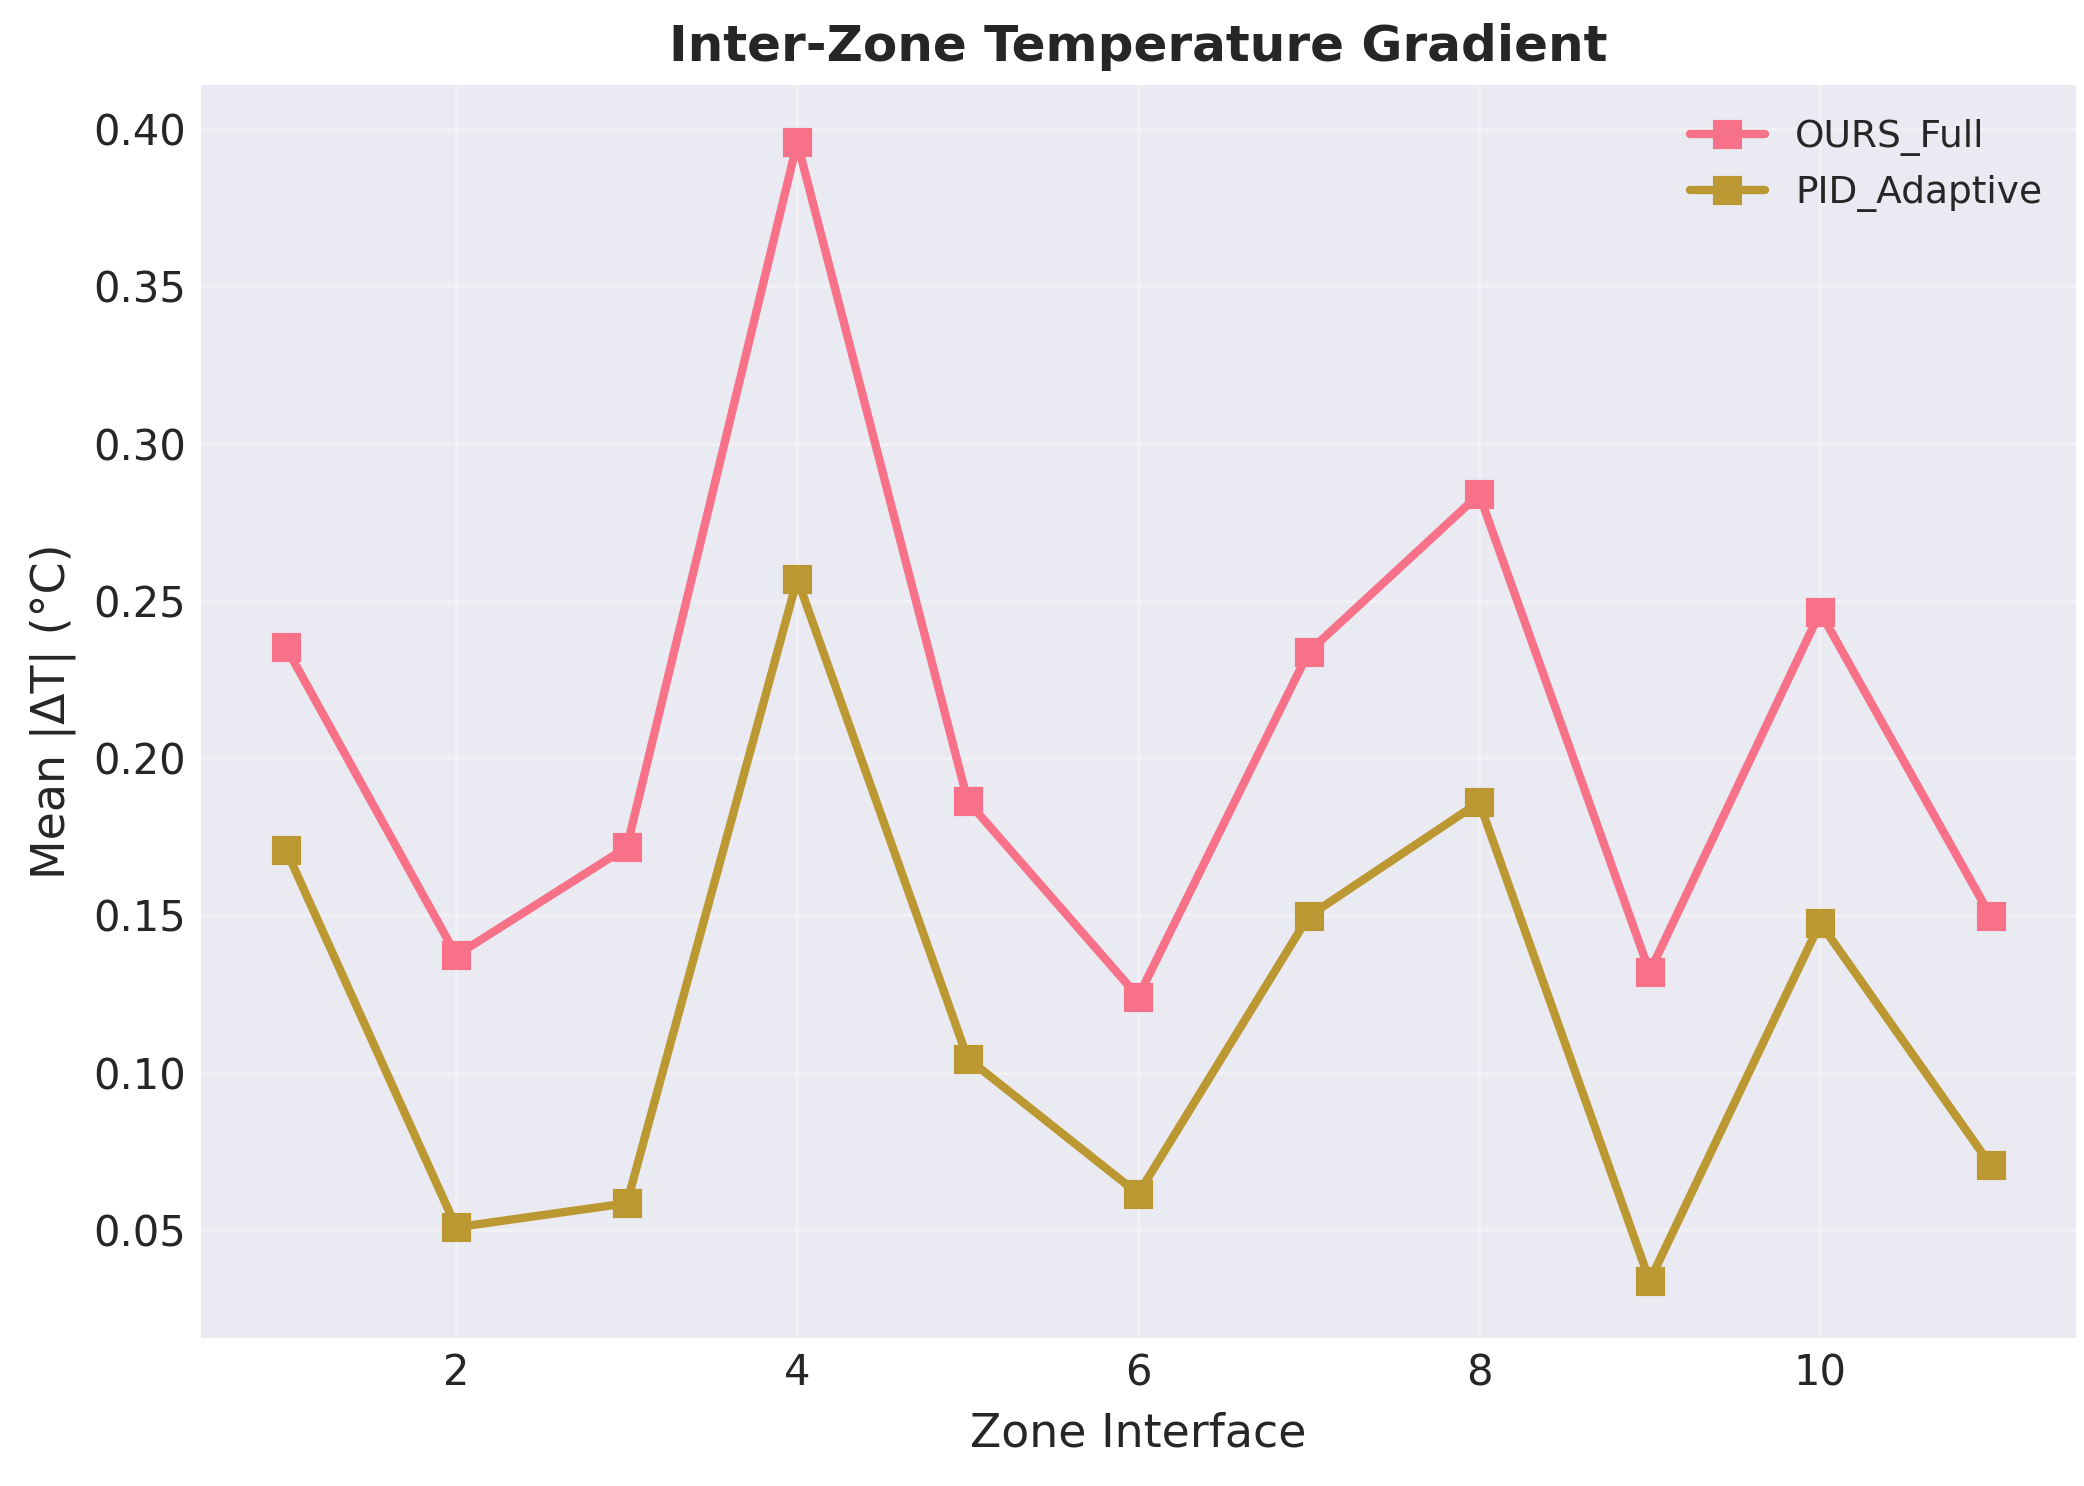
\includegraphics[width=0.8\linewidth]{analysis_spatial_patterns_r2c1.png}
    \caption{Spatial panel three. Spatiotemporal temperature map.}
    \label{fig:spatial_r2c1}
\end{figure}

\begin{figure}[htbp]
    \centering
    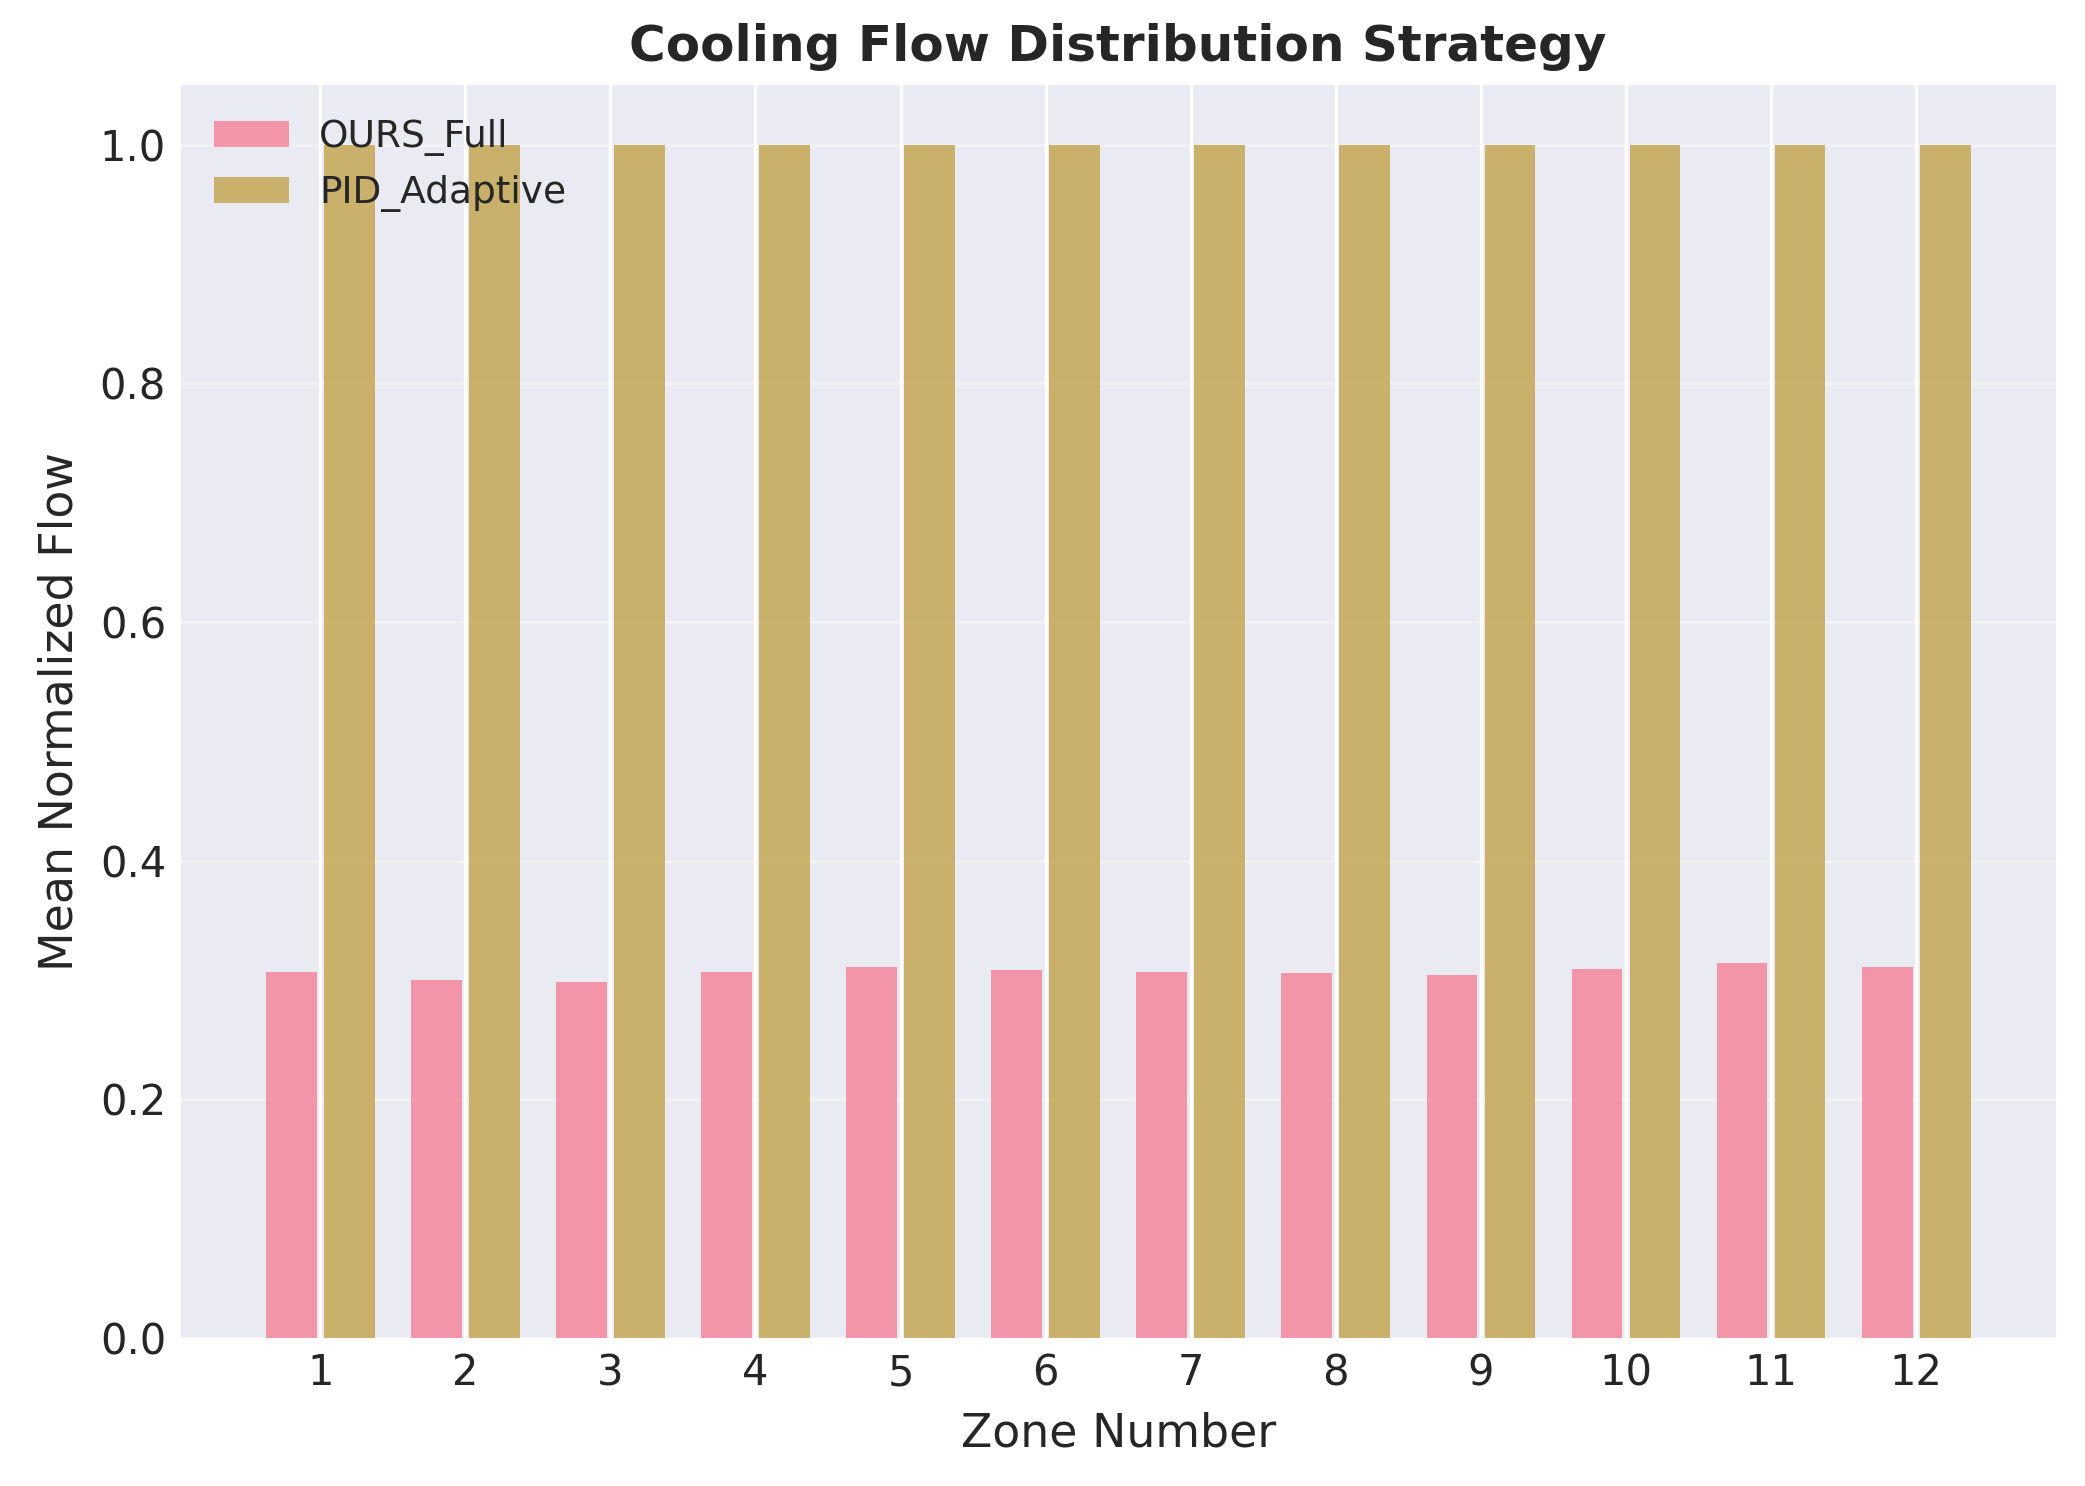
\includegraphics[width=0.8\linewidth]{analysis_spatial_patterns_r2c2.png}
    \caption{Spatial panel four. Zone wise cooling flow distribution.}
    \label{fig:spatial_r2c2}
\end{figure}

\paragraph{Spatiotemporal map and flow allocation}
Figures \ref{fig:spatial_r2c1} and \ref{fig:spatial_r2c2} link hotspot evolution with flow allocation.
Temperature maps show how hotspot locations move during changing demand periods.
Predictive methods target emerging hotspots with localized interventions at critical times.
Proportional control produces smoother maps through more uniform cooling deployment.
PID strategies suppress hotspots broadly using sustained high flow periods.
Flow allocation bars confirm these differences across control families.
Predictive methods allocate larger flow to zones with higher predicted risk.
Uniform methods distribute flow evenly and prioritize homogeneous temperature fields.
These allocation choices drive previously observed energy and spread outcomes.
The pair provides direct actuator level interpretation of controller behavior.
It supports practical calibration for safety constraints and energy budgets. Flow targeting can be tuned by zone risk and mission priorities. Calibration should preserve hotspot suppression without excessive global actuation. Map evidence shows where localized intervention is sufficient. This guidance helps convert analysis into actionable control settings. It also improves repeatability when teams tune controllers across different platforms.

\subsubsection{Multi metric synthesis}

\begin{figure}[htbp]
    \centering
    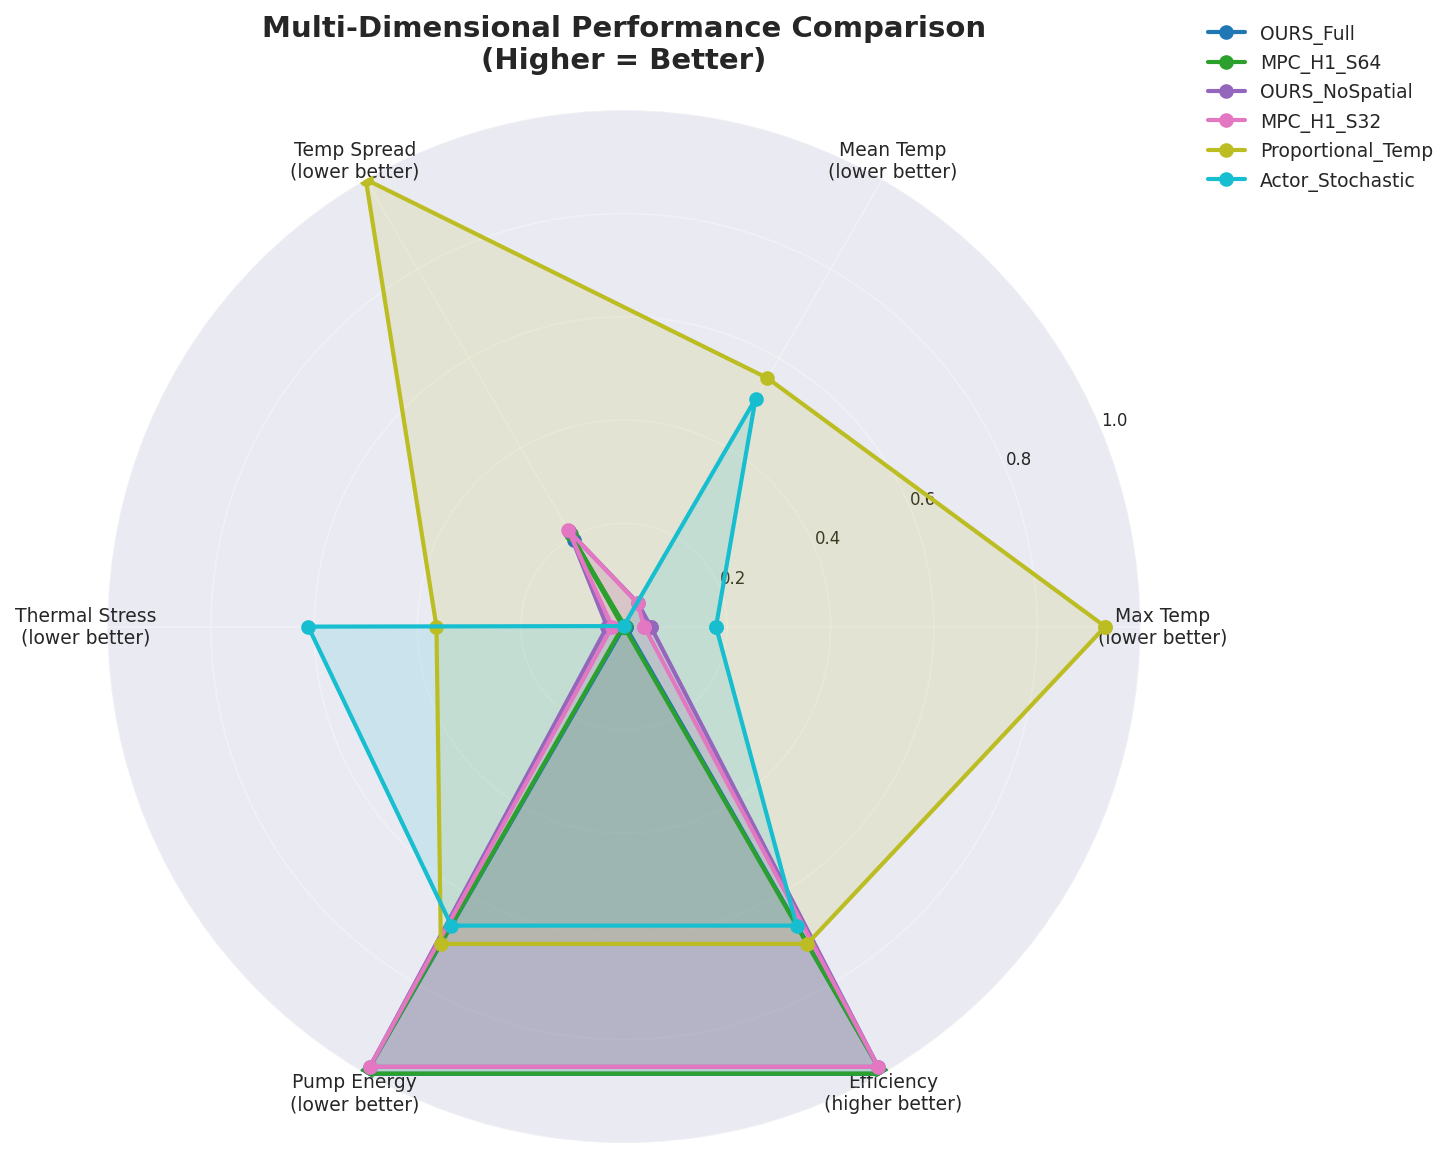
\includegraphics[width=0.8\linewidth]{radar_comparison.png}
    \caption{Radar comparison of normalized performance metrics.}
    \label{fig:radar_comparison}
\end{figure}

Figure \ref{fig:radar_comparison} combines normalized metrics into one comparative performance map.
Each radial axis represents one objective from the evaluation protocol.
Larger radial extent indicates stronger normalized performance for that objective.
Proportional control dominates temperature and uniformity related axes.
OURS Full and MPC variants dominate energy related axes.
PID methods retain thermal safety strength but lose efficiency competitiveness.
No method simultaneously maximizes every axis on this chart.
This confirms the multi objective nature of thermal control design.
Radar geometry highlights weaknesses that tables can hide during quick review.
It enables stakeholders to choose weights aligned with mission priorities.
The figure therefore summarizes trade structure before final ranking discussion. It offers a compact bridge between detailed panels and final synthesis. Designers can quickly identify dominant strengths and visible weaknesses. The map also supports communication with non specialist stakeholders. This makes cross team alignment faster during controller selection. It also reduces ambiguity when defining objective weights before final validation.

\subsubsection{Control action behavior}

\begin{figure}[htbp]
    \centering
    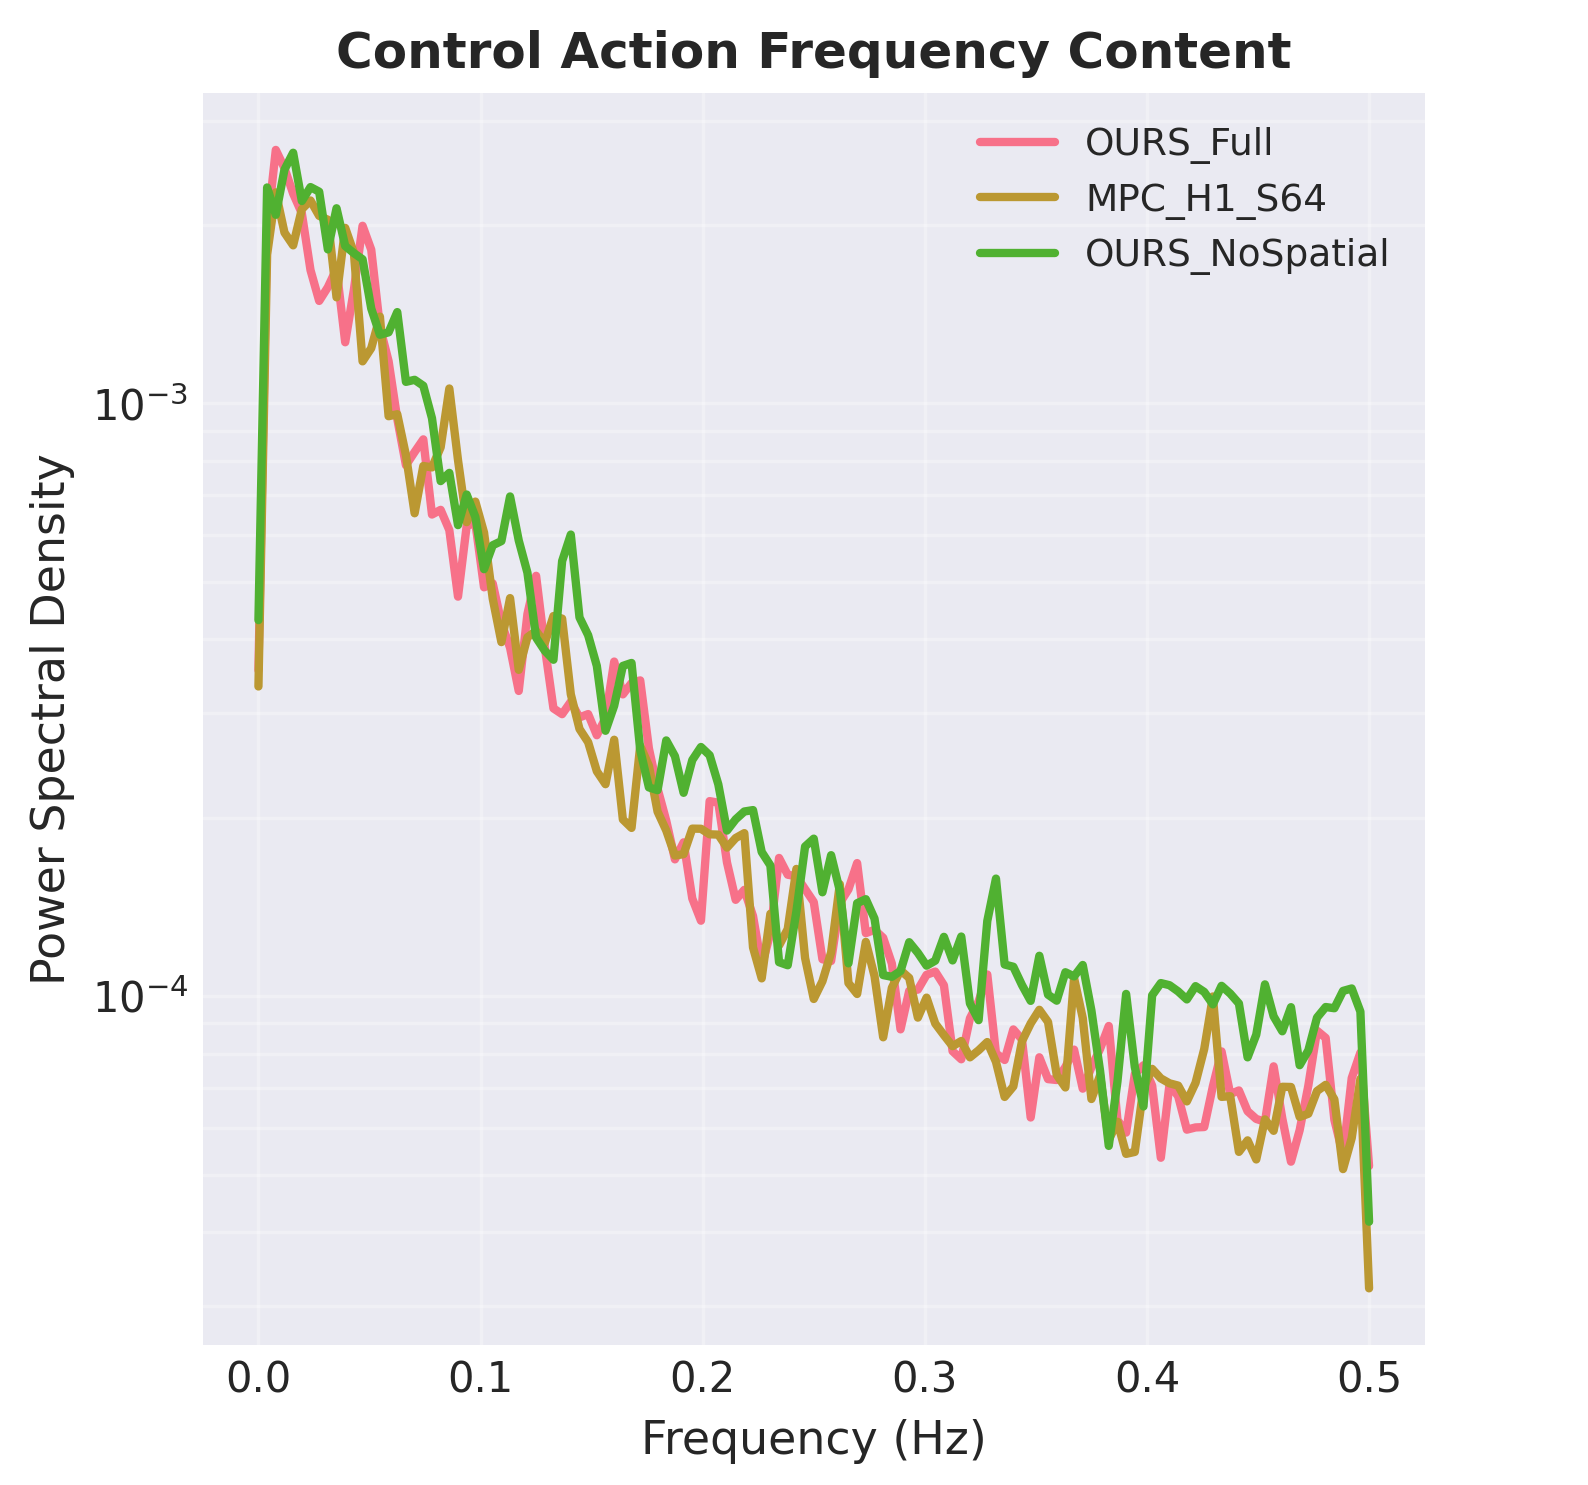
\includegraphics[width=0.8\linewidth]{analysis_control_behavior_r1c1.png}
    \caption{Control panel one. Action frequency spectrum.}
    \label{fig:control_r1c1}
\end{figure}

\begin{figure}[htbp]
    \centering
    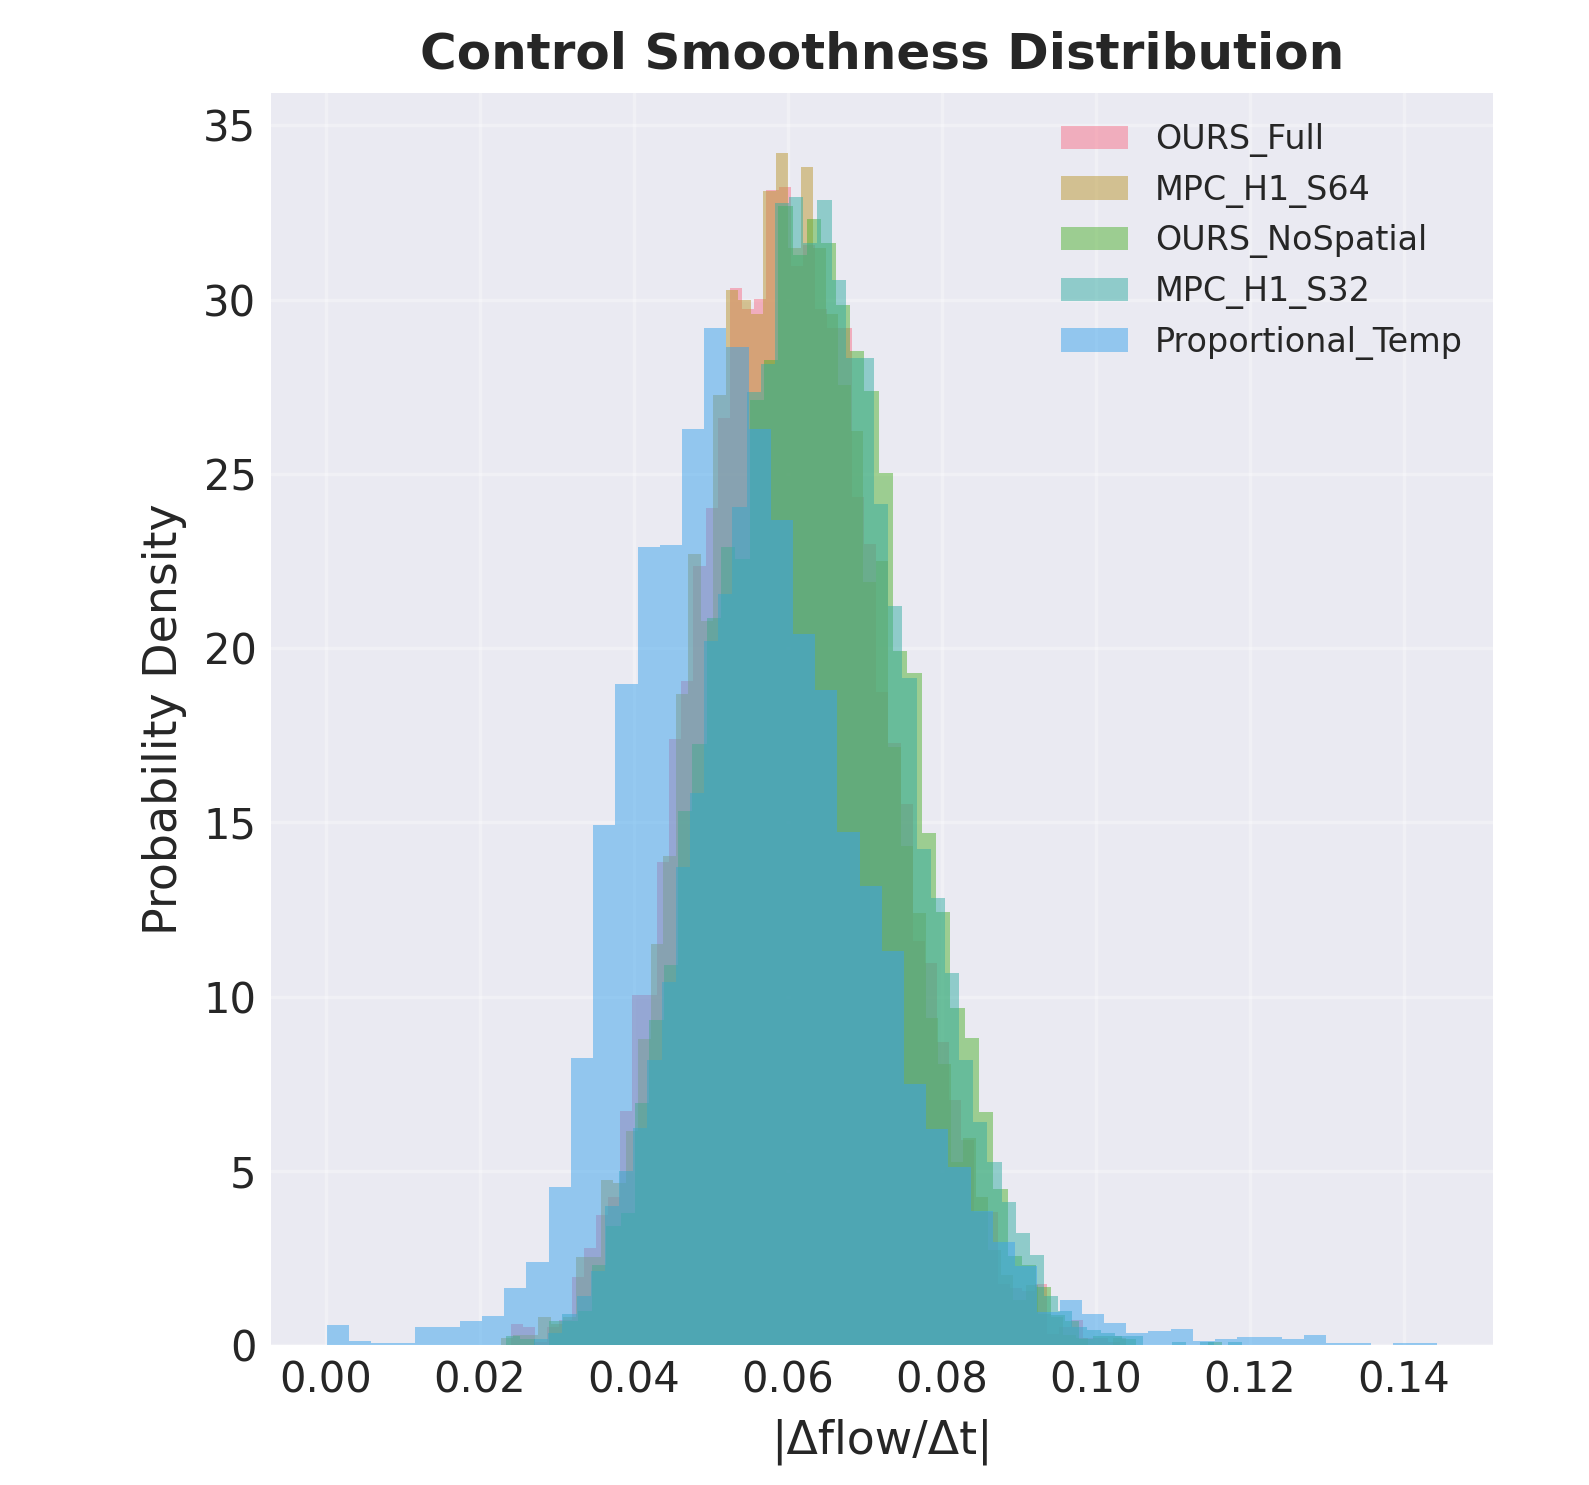
\includegraphics[width=0.8\linewidth]{analysis_control_behavior_r1c2.png}
    \caption{Control panel two. Action smoothness distribution.}
    \label{fig:control_r1c2}
\end{figure}

\paragraph{Frequency and smoothness}
Figures \ref{fig:control_r1c1} and \ref{fig:control_r1c2} describe action frequency and smoothness behavior.
Lower high frequency content indicates fewer rapid command oscillations.
Predictive methods reduce high frequency content compared with PID methods.
Smoothness distributions show predictive methods centered around moderate action changes.
Proportional control also exhibits stable increments across most intervals.
PID methods show wider tails and sharper command updates.
Sharper updates can increase actuator wear and acoustic disturbance.
Frequency and smoothness evidence aligns with temporal variability observations.
These plots therefore connect policy structure with hardware stress implications.
They support selecting controllers that balance responsiveness with mechanical longevity.
This pair provides strong practical value for maintenance aware deployment. Mechanical longevity depends strongly on oscillation frequency and command smoothness. Lower oscillation can reduce valve fatigue and pump stress accumulation. These benefits complement energy savings from moderated control action. Together they strengthen real world deployment viability. They also reduce unexpected maintenance burden during long fleet operation periods.

\begin{figure}[htbp]
    \centering
    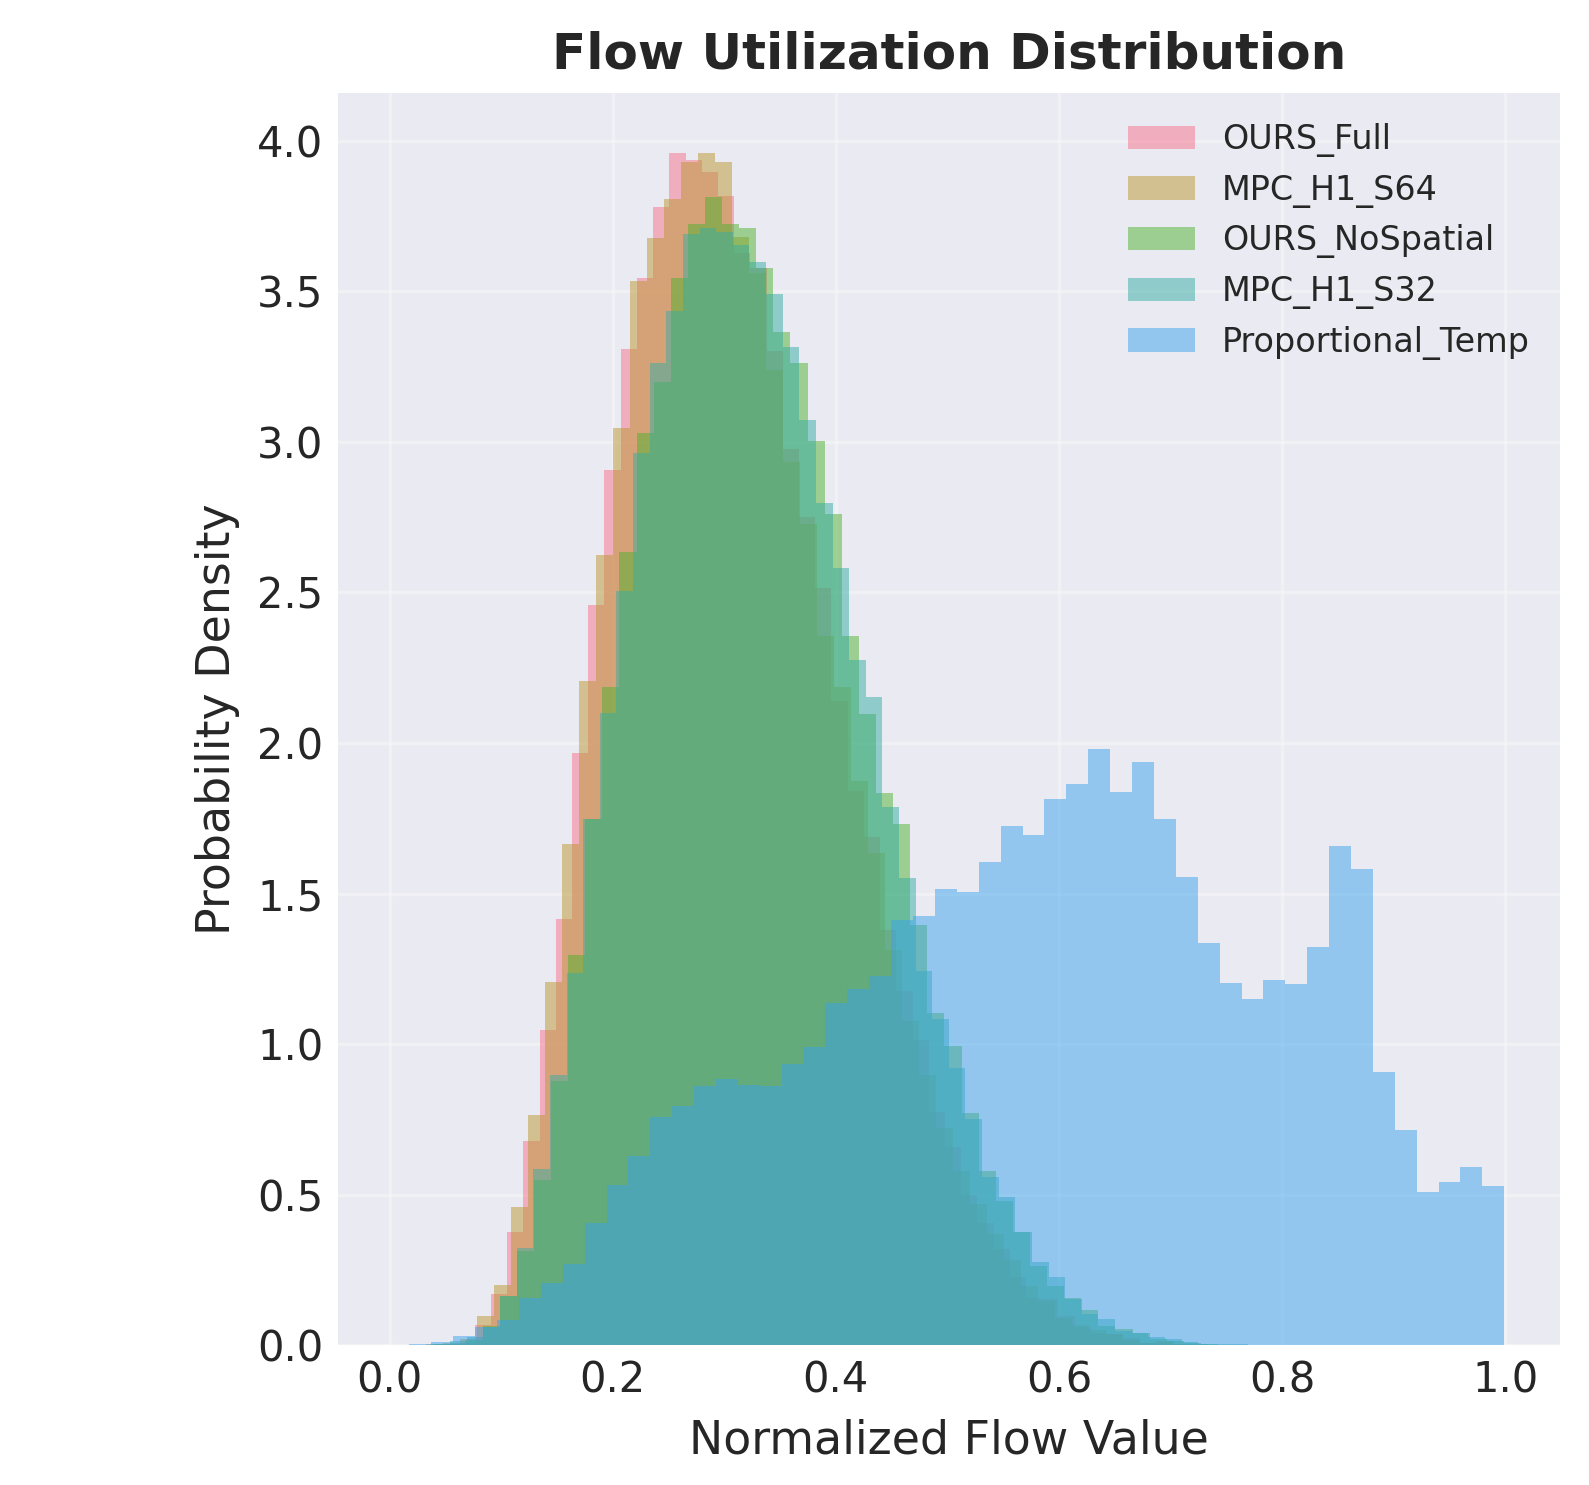
\includegraphics[width=0.8\linewidth]{analysis_control_behavior_r1c3.png}
    \caption{Control panel three. Flow utilization distribution.}
    \label{fig:control_r1c3}
\end{figure}

\begin{figure}[htbp]
    \centering
    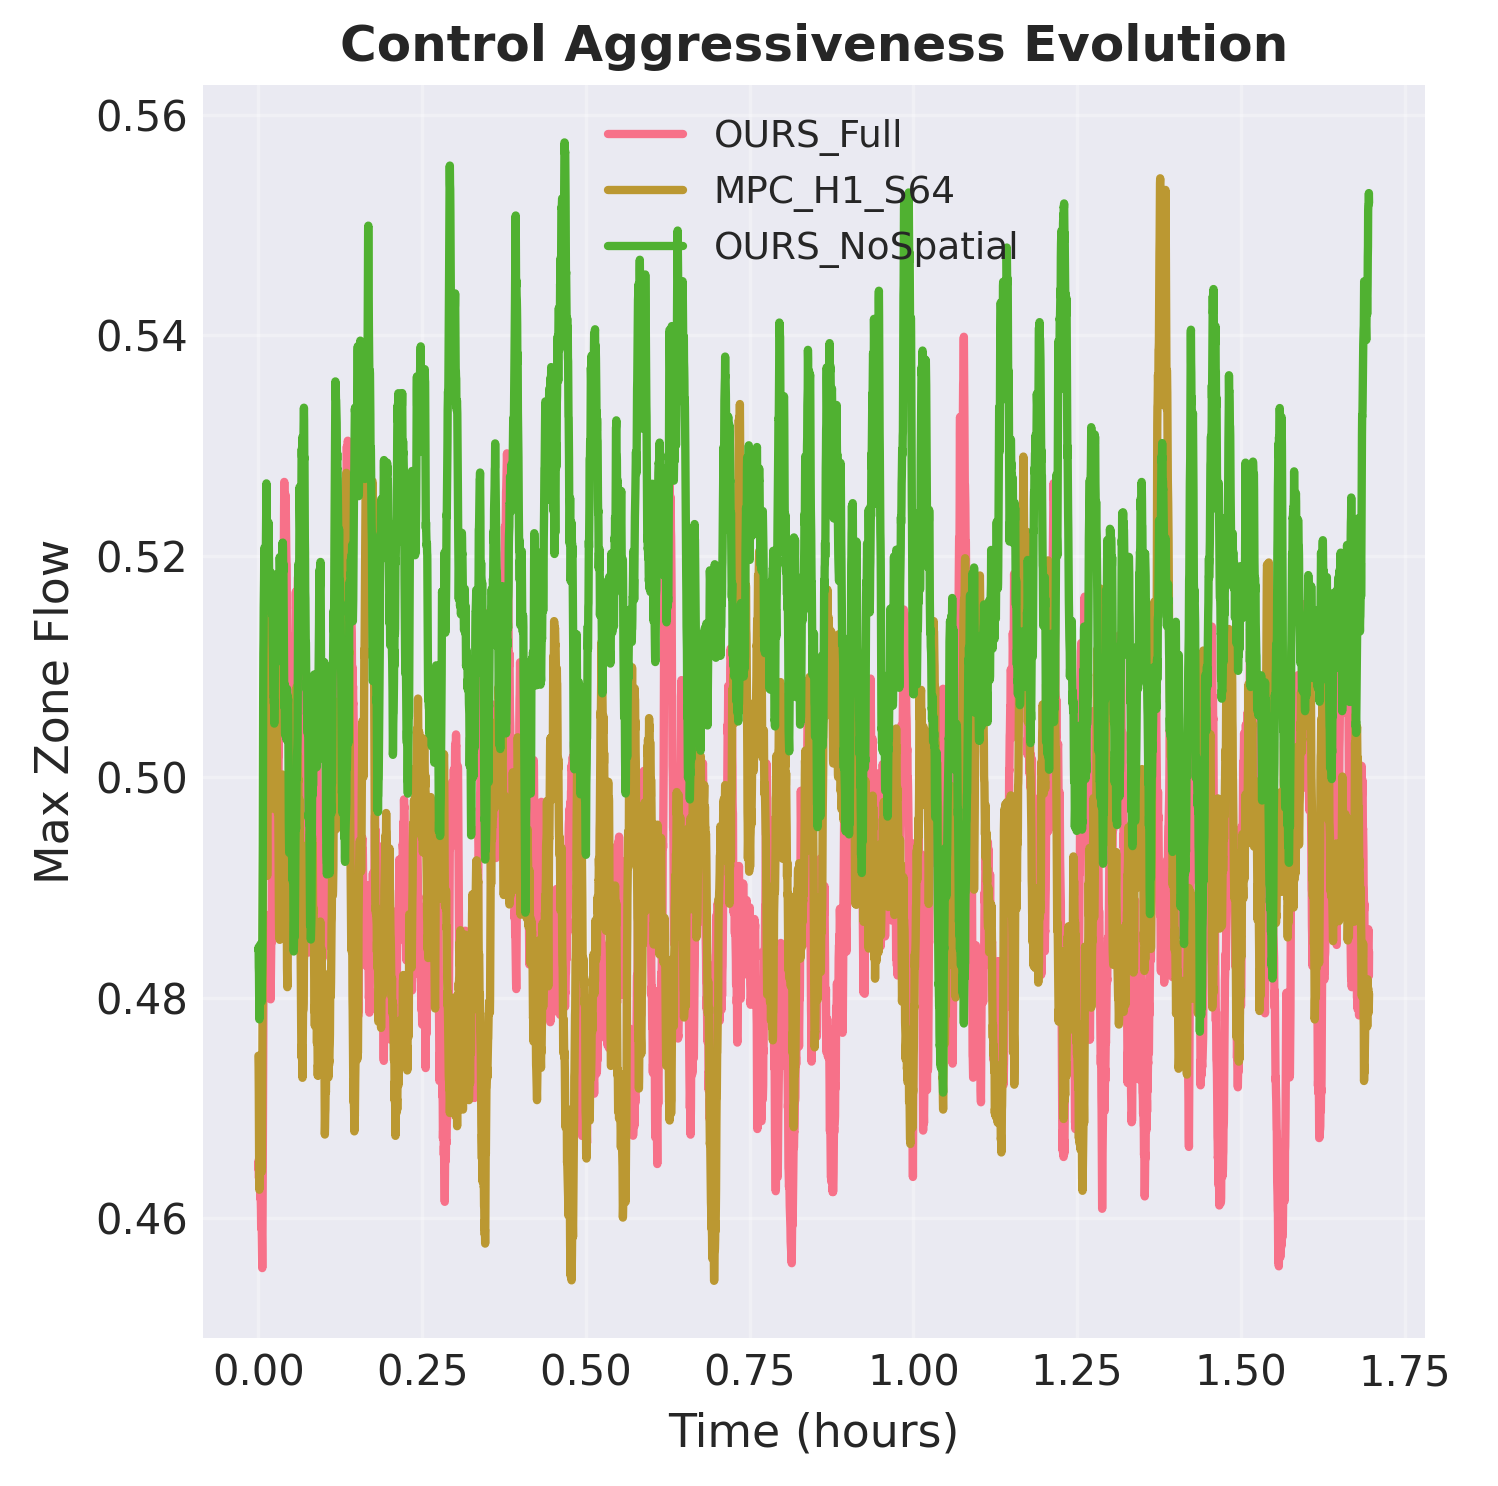
\includegraphics[width=0.8\linewidth]{analysis_control_behavior_r2c1.png}
    \caption{Control panel four. Control aggressiveness over time.}
    \label{fig:control_r2c1}
\end{figure}

\paragraph{Utilization and aggressiveness}
Figures \ref{fig:control_r1c3} and \ref{fig:control_r2c1} compare utilization and aggressiveness trends.
Utilization distributions indicate how strongly each method uses cooling authority.
Predictive methods span broader ranges while avoiding persistent maximum operation.
Proportional control stays near moderate utilization through most segments.
PID methods remain aggressive and operate near high utilization more frequently.
Aggressiveness traces show predictive methods increase action near anticipated risk events.
PID methods stay elevated longer, even after immediate risk subsides.
Extended high actuation explains higher cumulative cooling energy consumption.
Balanced aggressiveness supports efficiency without sacrificing thermal safety margins.
This pair explains timing quality differences between predictive and reactive policies.
It offers actionable guidance for aggressiveness limit tuning. Limits can be scheduled by predicted risk rather than fixed thresholds. This approach reduces unnecessary actuation during low risk intervals. It preserves rapid response when thermal risk increases suddenly. Such tuning improves efficiency while maintaining safety performance. It also preserves actuator health during repeated transient demand episodes.

\begin{figure}[htbp]
    \centering
    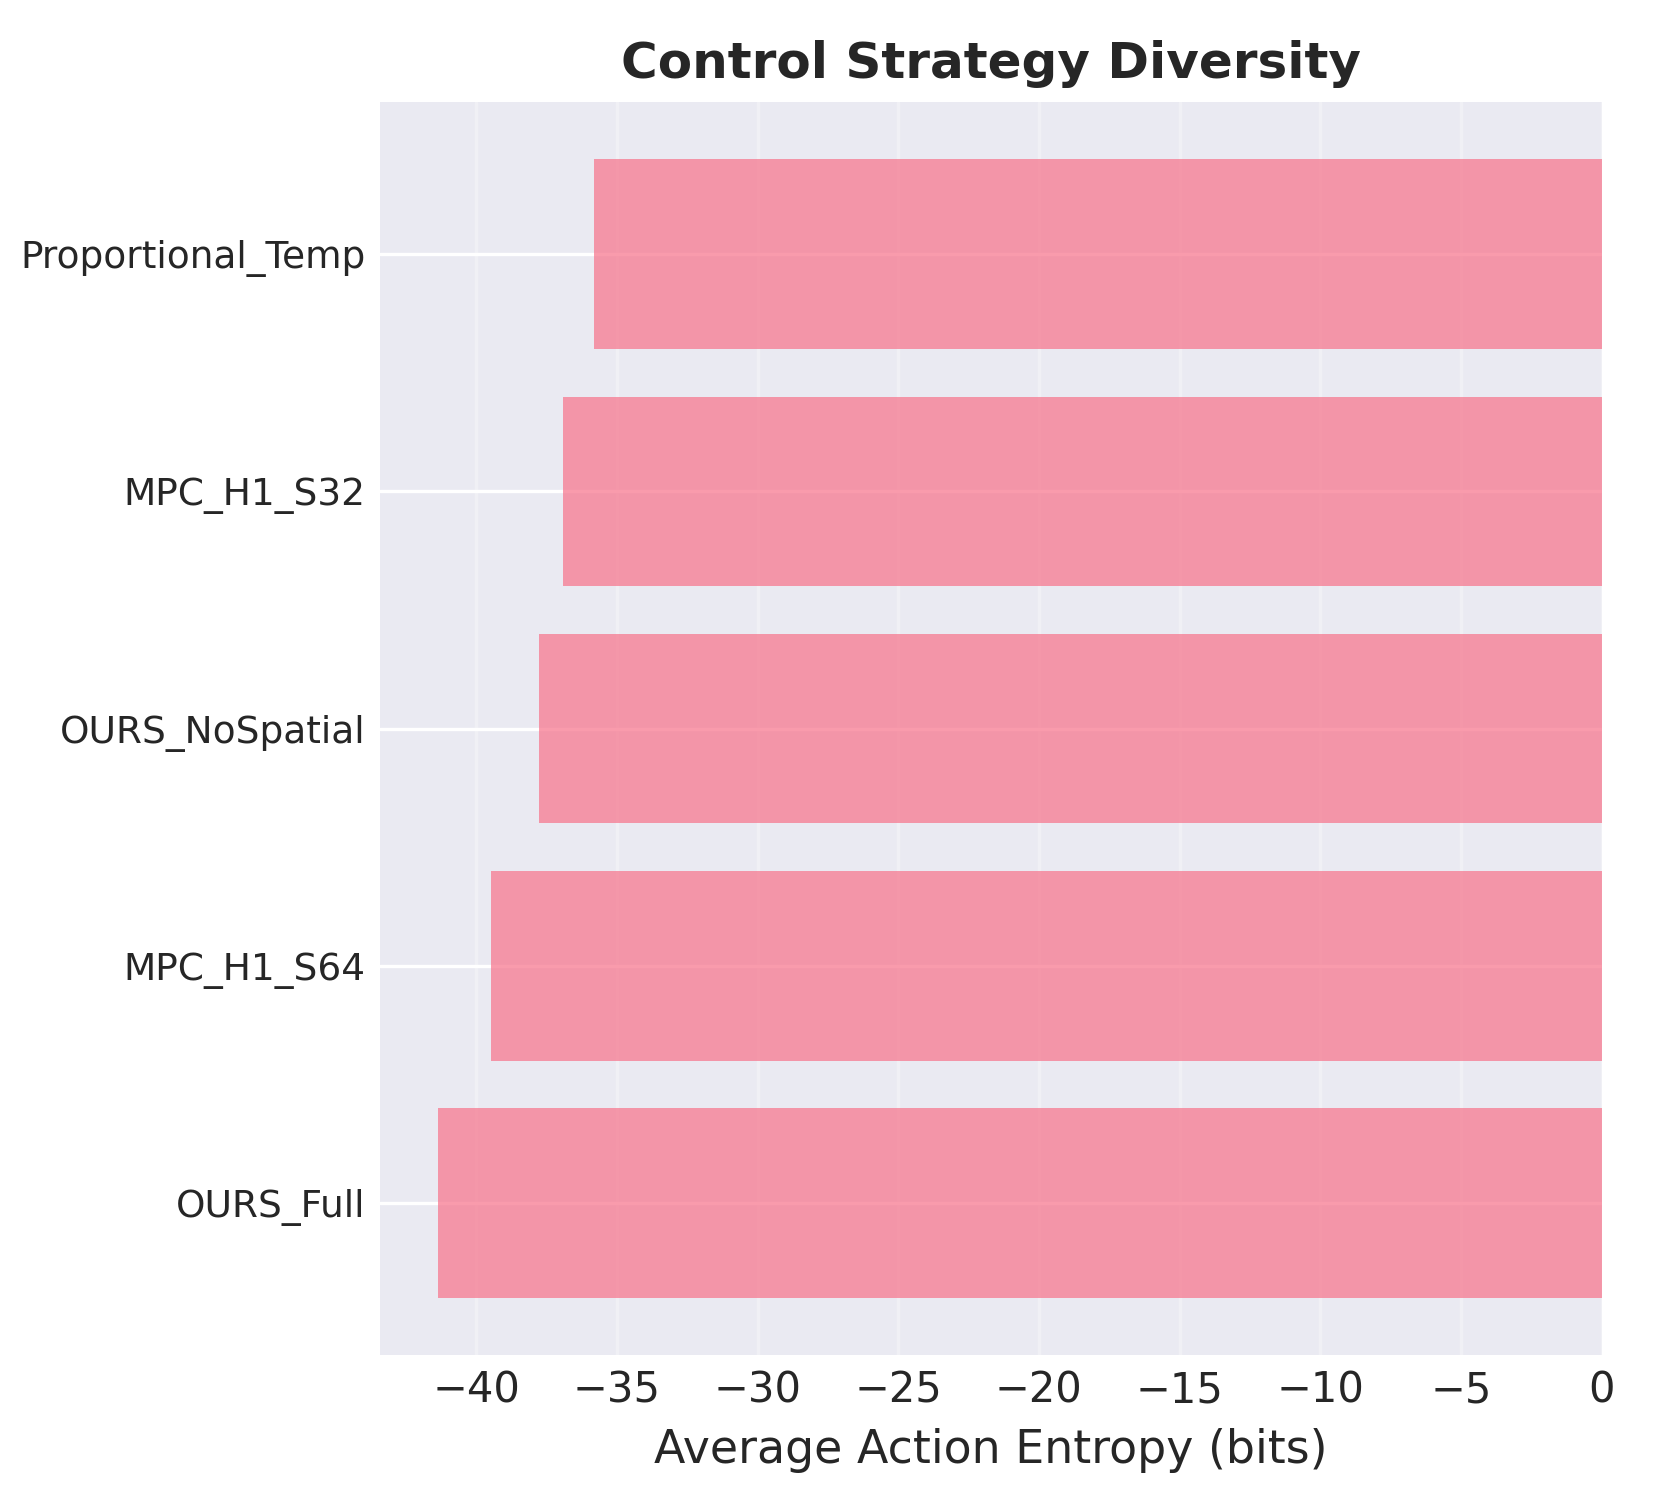
\includegraphics[width=0.8\linewidth]{analysis_control_behavior_r2c2.png}
    \caption{Control panel five. Control strategy diversity and response speed.}
    \label{fig:control_r2c2}
\end{figure}

\paragraph{Diversity and response speed}
Figure \ref{fig:control_r2c2} compares strategy diversity together with response speed indicators.
Higher diversity reflects broader action patterns across changing operating contexts.
Predictive actor methods maintain meaningful diversity with fast corrective response.
Proportional control responds quickly but explores narrower strategy space.
PID methods react quickly with repetitive high intensity corrections.
Diversity helps adaptation when operating conditions differ from training contexts.
Fast response preserves safety during sudden thermal rise events.
Balanced diversity and speed therefore represent a desirable control characteristic.
This figure suggests predictive learning methods approach that balanced behavior.
It complements frequency and utilization findings from preceding control panels.
The evidence supports robust deployment under variable real world usage. Diverse action patterns improve adaptation to unseen driving conditions. Response speed remains essential during abrupt thermal disturbances. Joint improvement across both properties indicates balanced control capability. This strengthens confidence for field level operation. It also supports stable behavior under broad ambient and traffic variation.

\subsubsection{Overall ranking}

Overall ranking aggregates temperature, spread, energy, and overhead behavior into one synthesis view.
Proportional control achieves the strongest combined rank under current weighting choices.
OURS Full and MPC variants follow closely through efficient auxiliary energy behavior.
PID methods rank lower because their cooling demand remains consistently high.
Actor based methods occupy intermediate positions with balanced metric performance.
Ranking should not be interpreted as universal dominance across missions.
Safety critical operation may prioritize lower peaks over strict energy minimization.
Range critical operation may prioritize overhead reduction and smoother actuation.
Panel level evidence explains why ranking positions differ across controller families.
Using ranking with figure level interpretation improves transparent decision making.
This combined approach supports defensible controller selection for practical deployment. It links ranking outcomes to observable mechanisms in every figure group. Decision makers can trace conclusions back to concrete evidence. That traceability improves confidence during validation and audit processes. The final narrative therefore remains rigorous, transparent, and implementation focused.


% ====================================================================
% ====================================================================
% ====================================================================

% === I. INTRODUCTION =============================================================


% ============================================================
% Replace external BibTeX with an inline bibliography as requested
% (highlighted)
\begin{thebibliography}{99}

\bibitem{Welsby2021}
D. Welsby, J. Price, S. Pye, and P. Ekins, ``Unextractable fossil fuels in a 1.5 °C world,'' \textit{Nature}, vol. 597, no. 7875, pp. 230--234, 2021, doi:10.1038/s41586-021-03821-8.

\bibitem{Bersalli2023}
G. Bersalli, T. Tr{\"o}ndle, and J. Lilliestam, ``Most industrialised countries have peaked carbon dioxide emissions during economic crises through strengthened structural change,'' \textit{Commun. Earth Environ.}, vol. 4, no. 1, p. 44, 2023, doi:10.1038/s43247-023-00687-8.

\bibitem{LCA_EV2023}
Y. Wang \textit{et al.}, ``Life cycle environmental impact assessment for battery-powered electric vehicles at the global and regional levels,'' \textit{Scientific Reports}, vol. 13, no. 1, p. 8491, 2023, doi:10.1038/s41598-023-35150-3.

\bibitem{AirQuality_EV2023}
W. Liu \textit{et al.}, ``Impact of battery electric vehicle usage on air quality in three Chinese first-tier cities,'' \textit{Scientific Reports}, vol. 13, no. 1, p. 20617, 2023, doi:10.1038/s41598-023-50745-6.

\bibitem{Link2024}
S. Link \textit{et al.}, ``Declining Costs Imply Fast Market Uptake of Zero-emission Trucks,'' \textit{Nature Energy}, vol. 9, no. 8, pp. 924--925, 2024, doi:10.1038/s41560-024-01555-1.

\bibitem{ThermalGradients2023}
X. Zhang \textit{et al.}, ``Effect of thermal gradients on inhomogeneous degradation in lithium-ion batteries,'' \textit{Communications Engineering}, vol. 2, no. 1, p. 45, 2023, doi:10.1038/s44172-023-00124-w.

\bibitem{MultiscaleCoupling2022}
H. Li \textit{et al.}, ``Multiscale coupling of surface temperature with solid diffusion in large lithium-ion pouch cells,'' \textit{Communications Engineering}, vol. 1, no. 1, p. 5, 2022, doi:10.1038/s44172-022-00005-8.

\bibitem{OperandoRunaway2023}
P. Di Palma \textit{et al.}, ``Operando monitoring of thermal runaway in commercial lithium-ion cells via advanced lab-on-fiber technologies,'' \textit{Nature Communications}, vol. 14, no. 1, p. 5715, 2023, doi:10.1038/s41467-023-40995-3.

\bibitem{11017253}
N. Aksoy, F. Cakil, and M. Ozden, ``Optimizing Battery Cooling with Reinforcement Learning: A Dynamic Control Strategy for Energy Storage Systems,'' in \textit{2025 7th International Congress on Human-Computer Interaction, Optimization and Robotic Applications (ICHORA)}, 2025, pp. 1--6, doi:10.1109/ICHORA65333.2025.11017253.

\bibitem{Huang2022}
G. Huang, P. Zhao, and G. Zhang, ``Real-Time Battery Thermal Management for Electric Vehicles Based on Deep Reinforcement Learning,'' \textit{IEEE Internet of Things Journal}, vol. 9, no. 15, pp. 14060--14072, 2022, doi:10.1109/JIOT.2022.3145849.

\bibitem{Wu2025}
C. Wu, J. Peng, J. Zhou, X. Guo, H. Guo, and C. Ma, ``Thermal Management Methodology Based on a Hybrid Deep Deterministic Policy Gradient With Memory Function for Battery Electric Vehicles in Hot Weather Conditions,'' \textit{IEEE Trans. Transp. Electrification}, vol. 11, no. 3, pp. 7232--7242, 2025, doi:10.1109/TTE.2024.3525014.

\bibitem{Cao2025}
G. Cao, Y. Jia, and J. Gao, ``Integrated Thermal Management Methodology Based on Proximal Policy Optimization With Memory Function for Battery Electric Vehicles,'' \textit{IEEE Access}, vol. 13, pp. 125180--125189, 2025, doi:10.1109/ACCESS.2025.3589659.

\bibitem{Rudolf2024}
T. Rudolf \textit{et al.}, ``Scenario-based Thermal Management Parametrization Through Deep Reinforcement Learning,'' arXiv:2408.02022, 2024. [Online]. Available: https://arxiv.org/abs/2408.02022.

\bibitem{Knehr2023}
K. W. Knehr and S. Ahmed, ``A New Analytical Expression for Estimating the Adiabatic Temperature Rise in Lithium-Ion Batteries During High-Power Pulses,'' \textit{Journal of The Electrochemical Society}, vol. 170, no. 2, p. 020515, 2023, doi:10.1149/1945-7111/acb849.

\bibitem{Liu2024}
Z. Liu \textit{et al.}, ``Physics-informed Machine Learning for Battery Pack Thermal Management,'' arXiv:2411.09915, 2024. [Online]. Available: https://arxiv.org/abs/2411.09915.

\bibitem{LiuFuzzy2023}
Z. Liu \textit{et al.}, ``Thermal Management with Fast Temperature Convergence Based on Optimized Fuzzy PID Algorithm for Electric Vehicle Battery,'' \textit{Applied Energy}, vol. 352, p. 121936, 2023, doi:10.1016/j.apenergy.2023.121936.

\bibitem{Ma2021}
Y. Ma \textit{et al.}, ``Battery Thermal Management Strategy for Electric Vehicles Based on Nonlinear Model Predictive Control,'' \textit{Measurement}, vol. 186, p. 110115, 2021, doi:10.1016/j.measurement.2021.110115.

\bibitem{Ali2024}
Z. M. Ali \textit{et al.}, ``Advancements in Battery Thermal Management for Electric Vehicles: Types, Technologies, and Control Strategies Including Deep Learning Methods,'' \textit{Ain Shams Engineering Journal}, vol. 15, no. 9, p. 102908, 2024, doi:10.1016/j.asej.2024.102908.

\bibitem{Batteries2023}
H. Zhang, J. Zhang, T. Song, X. Zhao, Y. Zhang, and S. Zhao, ``Optimization of Battery Thermal Management for Real Vehicles via Driving Condition Prediction Using Neural Networks,'' \textit{Batteries}, vol. 11, no. 6, p. 224, 2025, doi:10.3390/batteries11060224.

\bibitem{ESWA2025}
X. Guo, J. Peng, H. He, C. Wu, H. Zhang, and C. Ma, ``Integrated Thermal-Energy Management for Electric Vehicles in High-Temperature Conditions Using Hierarchical Reinforcement Learning (HGO-DDPG-E),'' \textit{Expert Systems with Applications}, vol. 276, p. 127221, 2025, doi:10.1016/j.eswa.2025.127221.

\bibitem{WRAP2025}
K. Li \textit{et al.}, ``Reinforcement Learning-Based Hyperparameter Tuning for Battery Thermal Management: Adaptive MPC + SAC,'' University of Warwick WRAP Repository, 2025. [Online]. Available: https://wrap.warwick.ac.uk/191337/.

\bibitem{RSC2025}
Y. Zhang, J. Huang, L. He, D. Zhao, and Y. Zhao, ``Reinforcement Learning-Based Control for the Thermal Management of the Battery and Occupant Compartments of Electric Vehicles,'' \textit{Sustainable Energy \& Fuels}, vol. 8, no. 3, 2024, doi:10.1039/d3se01403g.

\bibitem{WEVJ2025}
K. Nam and C. Ahn, ``Energy-Efficient Battery Thermal Management in Electric Vehicles Using Artificial-Neural-Network-Based Model Predictive Control,'' \textit{World Electric Vehicle Journal}, vol. 16, no. 5, p. 279, 2025, doi:10.3390/wevj16050279.

\bibitem{IEEE10373609}
G. Cao, Y. Jia, and J. Gao, ``Integrated Thermal Management Methodology Based on Proximal Policy Optimization With Memory Function for Battery Electric Vehicles,'' \textit{IEEE Access}, vol. 13, p. 10373609, 2024, doi:10.1109/10373609.

\bibitem{Elsevier112466}
M. H. Abbasi, Z. Arjmandzadeh, J. Zhang, B. Xu, and V. Krovi, ``Deep Reinforcement Learning Based Fast Charging and Thermal Management Optimization of an Electric Vehicle Battery Pack,'' \textit{Journal of Energy Storage}, vol. 95, p. 112466, 2024, doi:10.1016/j.est.2024.112466.

\bibitem{Xu2019Thermoelectric}
H.-J. Xu, J.-X. Wang, Y.-Z. Li, and Y.-J. Bi, ``A Thermoelectric-Heat-Pump Employed Active Control Strategy for the Dynamic Cooling Ability Distribution of Liquid Cooling System for the Space Station's Main Power-Cell-Arrays,'' \textit{Entropy}, vol. 21, no. 6, p. 578, 2019, doi:10.3390/e21060578.

\bibitem{OrtizArevalo2024}
Y. Ortiz and P. Ar{\'e}valo \textit{et al.}, ``Recent Advances in Thermal Management Strategies for Lithium-Ion Batteries: A Comprehensive Review,'' \textit{Batteries}, vol. 10, no. 3, p. 83, 2024, doi:10.3390/batteries10030083.

\bibitem{EPA_Dynamometer}
United States Environmental Protection Agency,
Dynamometer Drive Schedules,
Vehicle and Fuel Emissions Testing web pages,
Accessed: 2026 02 26,
Available: https://www.epa.gov/vehicle-and-fuel-emissions-testing/dynamometer-drive-schedules. % :contentReference[oaicite:6]{index=6}

\bibitem{EPA_FTP}
United States Environmental Protection Agency,
EPA Federal Test Procedure FTP,
Emission standards reference guide,
Accessed: 2026 02 26,
Available: https://www.epa.gov/emission-standards-reference-guide/epa-federal-test-procedure-ftp. % :contentReference[oaicite:7]{index=7}

\bibitem{EPA_UDDS}
United States Environmental Protection Agency,
Urban Dynamometer Driving Schedule UDDS,
Emission standards reference guide,
Accessed: 2026 02 26,
Available: https://www.epa.gov/emission-standards-reference-guide/epa-urban-dynamometer-driving-schedule-udds. % :contentReference[oaicite:8]{index=8}

\bibitem{EPA_LA92}
United States Environmental Protection Agency,
LA92 Unified Dynamometer Driving Schedule,
Emission standards reference guide,
Accessed: 2026 02 26,
Available: https://www.epa.gov/emission-standards-reference-guide/la92-unified-dynamometer-driving-schedule. % :contentReference[oaicite:9]{index=9}

\bibitem{DieselNet_Cycles}
ECOpoint Inc, DieselNet,
Emission test cycles collection, including FTP75, UDDS, HWFET, US06, SC03, and LA92,
Accessed: 2026 02 26,
Available: https://dieselnet.com/standards/cycles/. % :contentReference[oaicite:10]{index=10}
\end{thebibliography}

\vfill

\end{document}
